\chapter{Appendix} 
\label{appendix}
%Title of the First Chapter

\ifpdf
    \graphicspath{{Appendix/Figs/Raster/}{Appendix/Figs/PDF/}{Appendix/Figs/}}
\else
    \graphicspath{{Appendix/Figs/Vector/}{Appendix/Figs/}}
\fi

This appendix collects complementary material that would interrupt the flow of this thesis.
Especially, it contains the images generated both from adversarial sampling techniques, both the ones generated using diffusion-based techniques. 
The collection of prompts used in the experiments follows.


\subsection{Adversarial Generated Images}
Tables~\ref{fig::advLC_CLSDIV0}, \ref{fig::advLC_CLSDIV1}, \ref{fig::advLC_NOCLSDIV0}, \ref{fig::advLC_NOCLSDIV1}, \ref{fig::advLF_CLSDIV0}, \ref{fig::advLF_CLSDIV1}, \ref{fig::advLF_NOCLSDIV0}, \ref{fig::advLF_NOCLSDIV1},
\ref{fig::advLT_CLSDIV0}, \ref{fig::advLT_CLSDIV1}, \ref{fig::advLT_NOCLSDIV0}, \ref{fig::advLT_NOCLSDIV1} show examples of transformations applied on Chin., Fren. and Turk. images from LAMP dataset with lamps turned off using PGD and CLSDIV or NOCLSDIV with Chin., Fren. and Turk as majority cultures.
% LAMP
%CLSDIV 0
\begin{figure}[H]
\centering
\begin{subfigure}[b]{0.6\columnwidth}
\centering
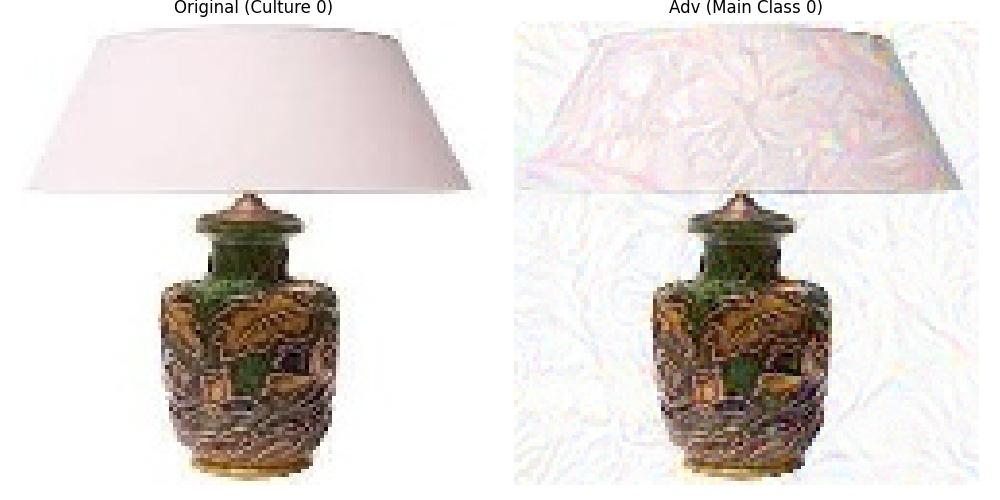
\includegraphics[width=\columnwidth]{adv_gen_figures/ADVmajLC_CLSDIV0_source_0.jpg}
\end{subfigure} \\
\begin{subfigure}[b]{0.6\columnwidth}
\centering
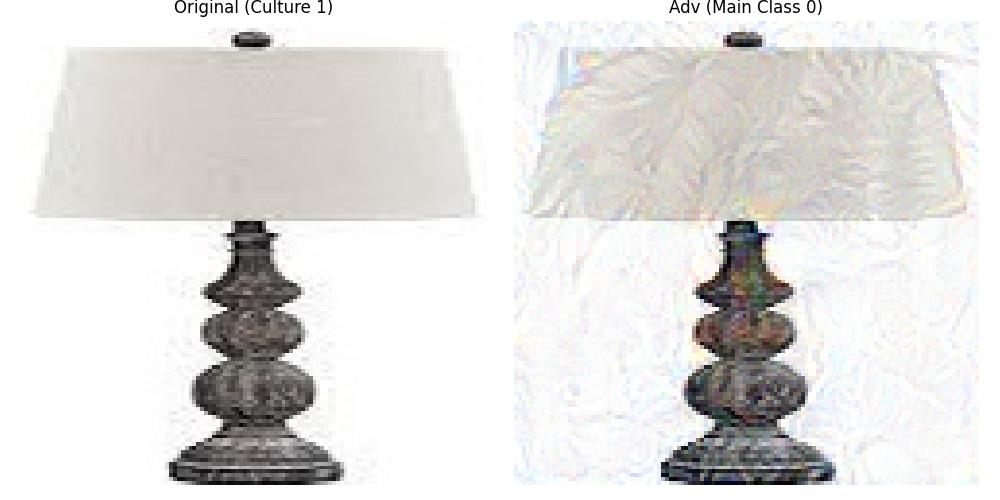
\includegraphics[width=\columnwidth]{adv_gen_figures/ADVmajLC_CLSDIV0_source_1.jpg}
\end{subfigure} \\
\begin{subfigure}[b]{0.6\columnwidth}
\centering
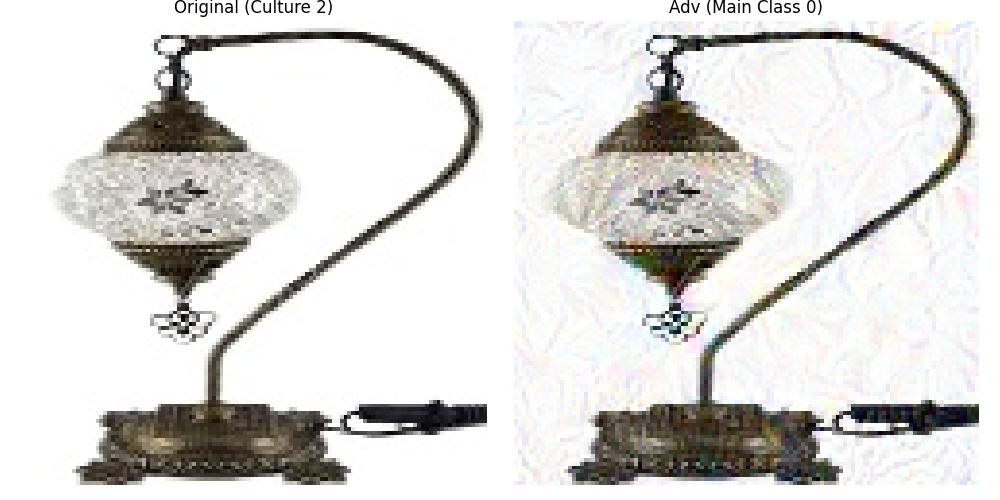
\includegraphics[width=\columnwidth]{adv_gen_figures/ADVmajLC_CLSDIV0_source_2.jpg}
\end{subfigure} 
\caption{Example of transformations applied on Chin., Fren. and Turk. images from LAMP dataset with lamps turned off using PGD and CLSDIV with Chin. as majority culture.}
\label{fig::advLC_CLSDIV0}
\end{figure}

\begin{figure}[H]
\centering
\begin{subfigure}[b]{0.6\columnwidth}
\centering
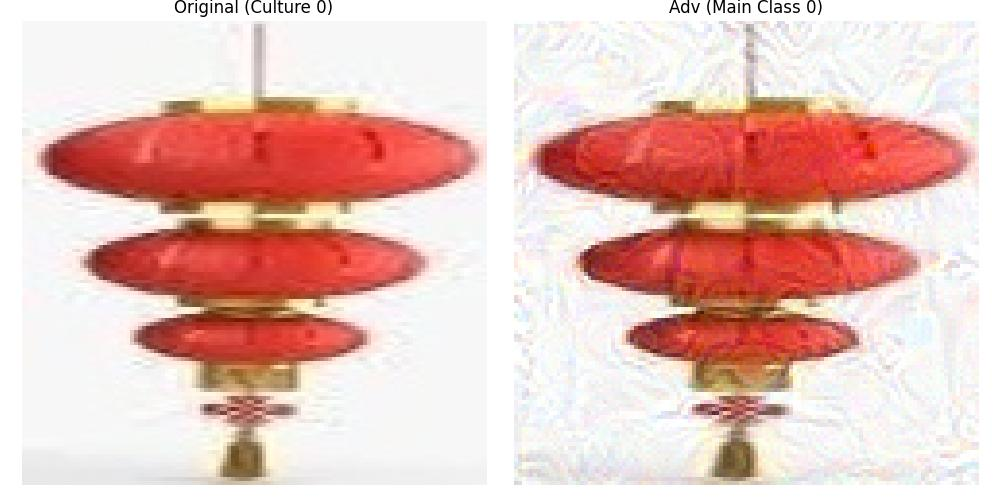
\includegraphics[width=\columnwidth]{adv_gen_figures/ADVmajLF_CLSDIV0_source_0.jpg}

\end{subfigure} \\
\begin{subfigure}[b]{0.6\columnwidth}
\centering
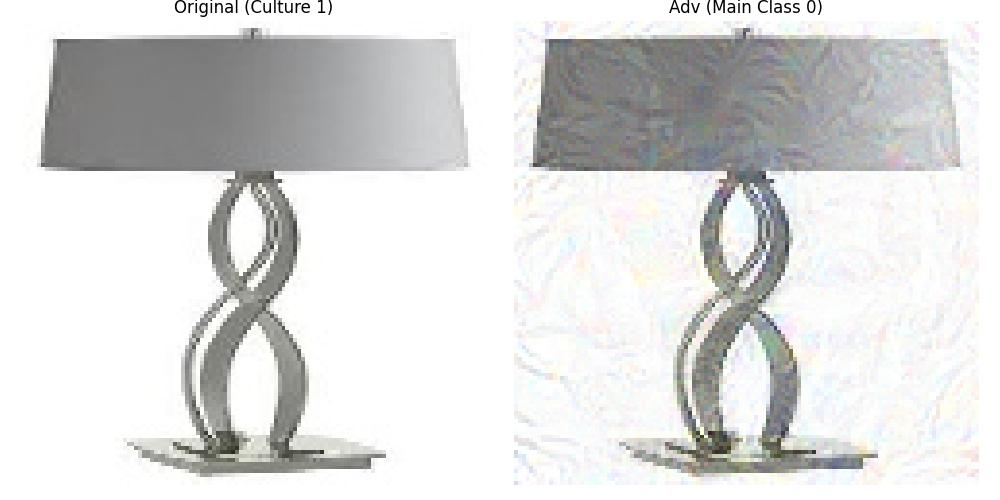
\includegraphics[width=\columnwidth]{adv_gen_figures/ADVmajLF_CLSDIV0_source_1.jpg}
\end{subfigure} \\
\begin{subfigure}[b]{0.6\columnwidth}
\centering
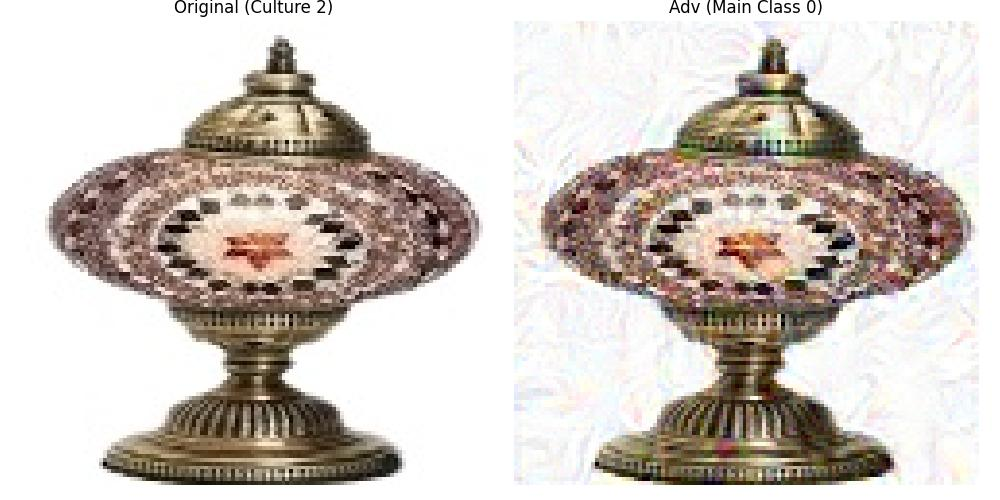
\includegraphics[width=\columnwidth]{adv_gen_figures/ADVmajLF_CLSDIV0_source_2.jpg}
\end{subfigure} 
\caption{Example of transformations applied on Chin., Fren. and Turk. images from LAMP dataset with lamps turned off using PGD and CLSDIV with Fren. as majority culture.}
\label{fig::advLF_CLSDIV0}
\end{figure}

\begin{figure}[H]
\centering
\begin{subfigure}[b]{0.6\columnwidth}
\centering
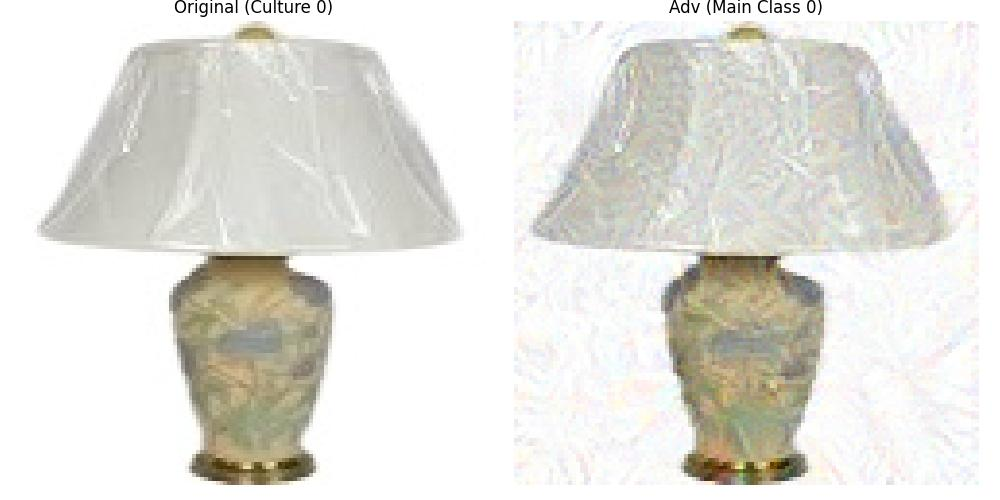
\includegraphics[width=\columnwidth]{adv_gen_figures/ADVmajLT_CLSDIV0_source_0.jpg}
\end{subfigure} \\
\begin{subfigure}[b]{0.6\columnwidth}
\centering
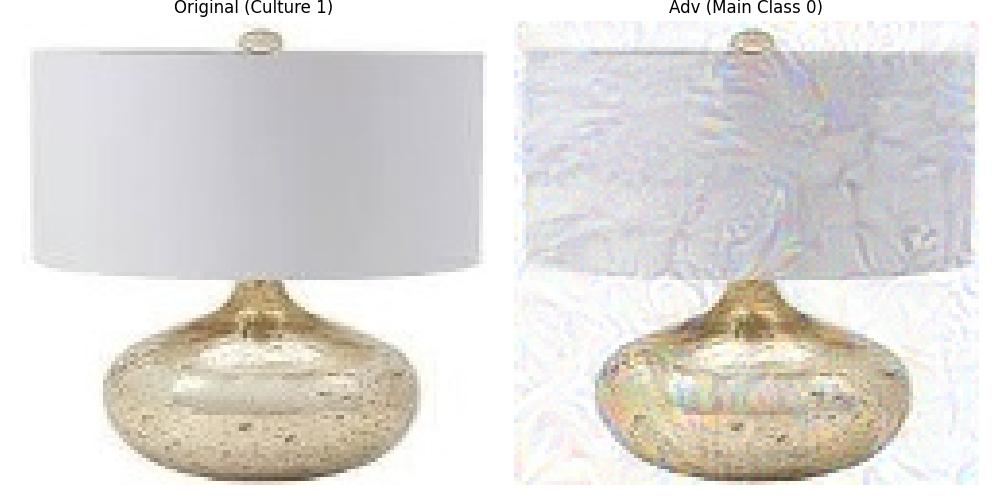
\includegraphics[width=\columnwidth]{adv_gen_figures/ADVmajLT_CLSDIV0_source_1.jpg}
\end{subfigure} \\
\begin{subfigure}[b]{0.6\columnwidth}
\centering
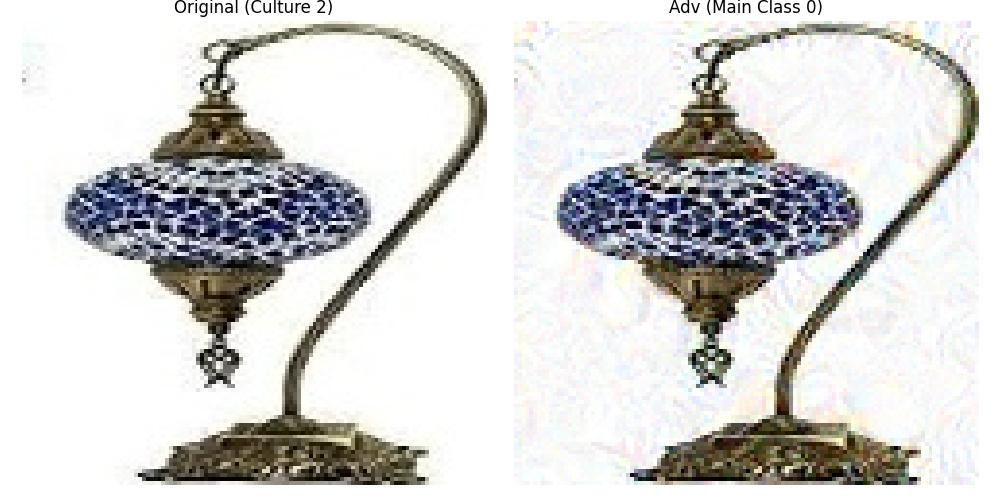
\includegraphics[width=\columnwidth]{adv_gen_figures/ADVmajLT_CLSDIV0_source_2.jpg}
\end{subfigure} 
\caption{Example of transformations applied on Chin., Fren. and Turk. images from LAMP dataset with lamps turned off using PGD and CLSDIV with Turk. as majority culture.}
\label{fig::advLT_CLSDIV0}
\end{figure}

%CLSDIV 1
\begin{figure}[H]
\centering
\begin{subfigure}[b]{0.6\columnwidth}
\centering
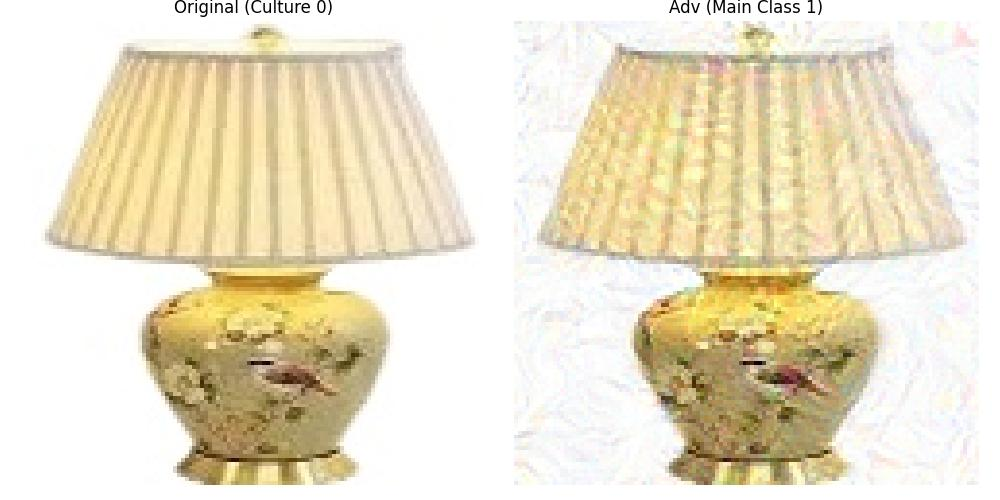
\includegraphics[width=\columnwidth]{adv_gen_figures/ADVmajLC_CLSDIV1_source_0.jpg}
\end{subfigure} \\
\begin{subfigure}[b]{0.6\columnwidth}
\centering
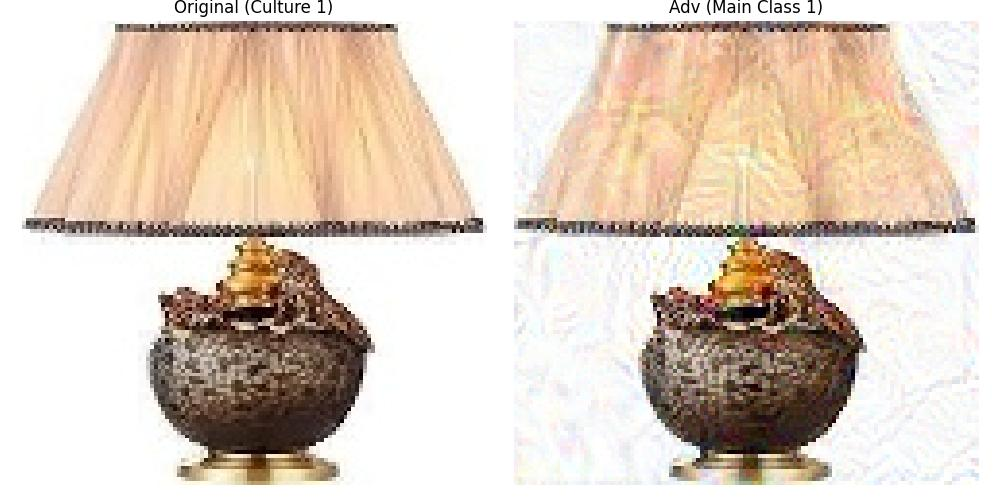
\includegraphics[width=\columnwidth]{adv_gen_figures/ADVmajLC_CLSDIV1_source_1.jpg}
\end{subfigure} \\
\begin{subfigure}[b]{0.6\columnwidth}
\centering
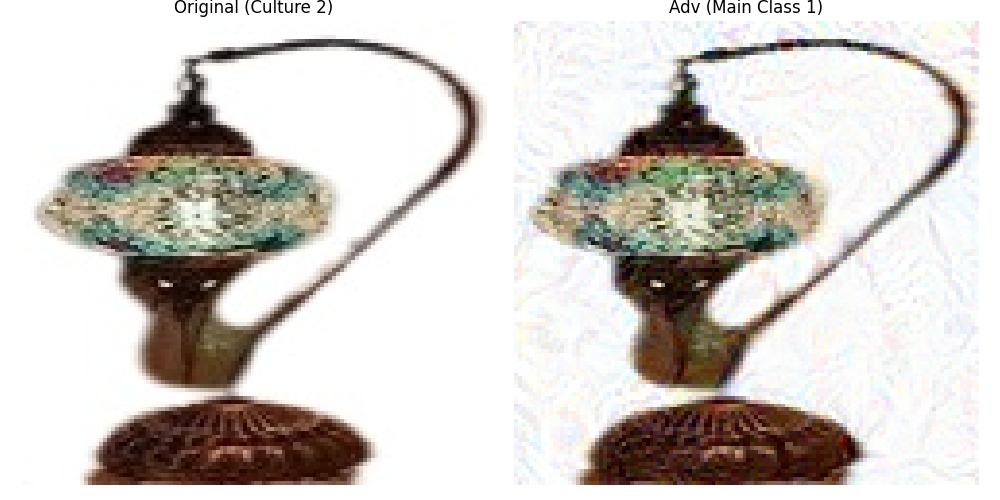
\includegraphics[width=\columnwidth]{adv_gen_figures/ADVmajLC_CLSDIV1_source_2.jpg}
\end{subfigure} 
\caption{Example of transformations applied on Chin., Fren. and Turk. images from LAMP dataset with lamps turned on using PGD and CLSDIV with Chin. as majority culture.}
\label{fig::advLC_CLSDIV1}
\end{figure}

\begin{figure}[H]
\centering
\begin{subfigure}[b]{0.6\columnwidth}
\centering
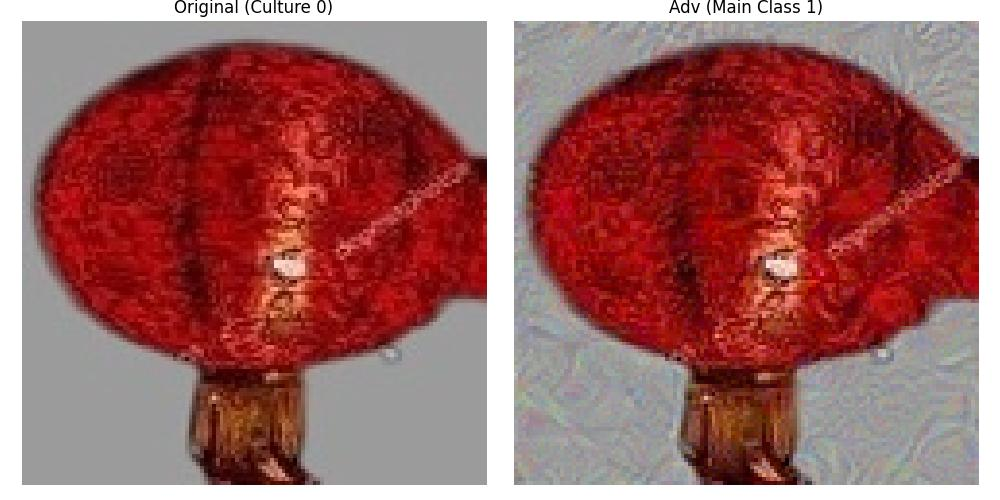
\includegraphics[width=\columnwidth]{adv_gen_figures/ADVmajLF_CLSDIV1_source_0.jpg}
\end{subfigure} \\
\begin{subfigure}[b]{0.6\columnwidth}
\centering
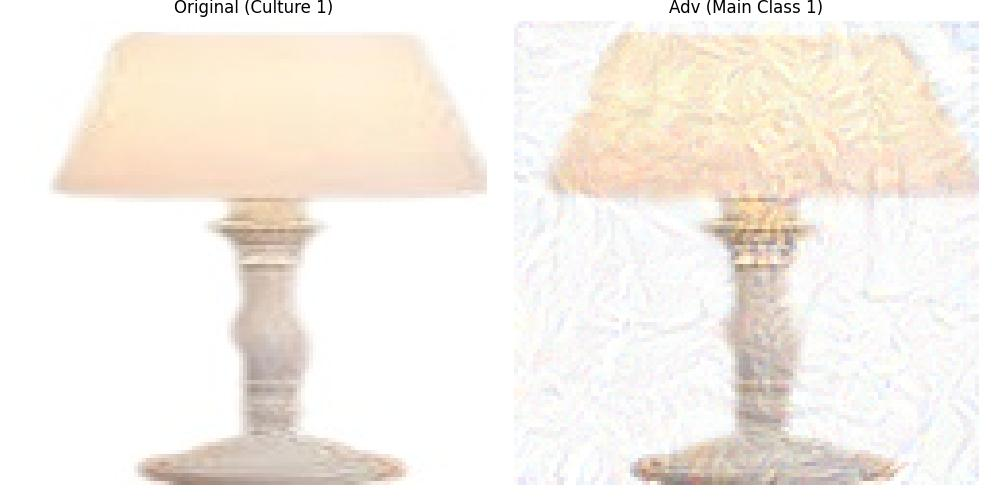
\includegraphics[width=\columnwidth]{adv_gen_figures/ADVmajLF_CLSDIV1_source_1.jpg}
\end{subfigure} \\
\begin{subfigure}[b]{0.6\columnwidth}
\centering
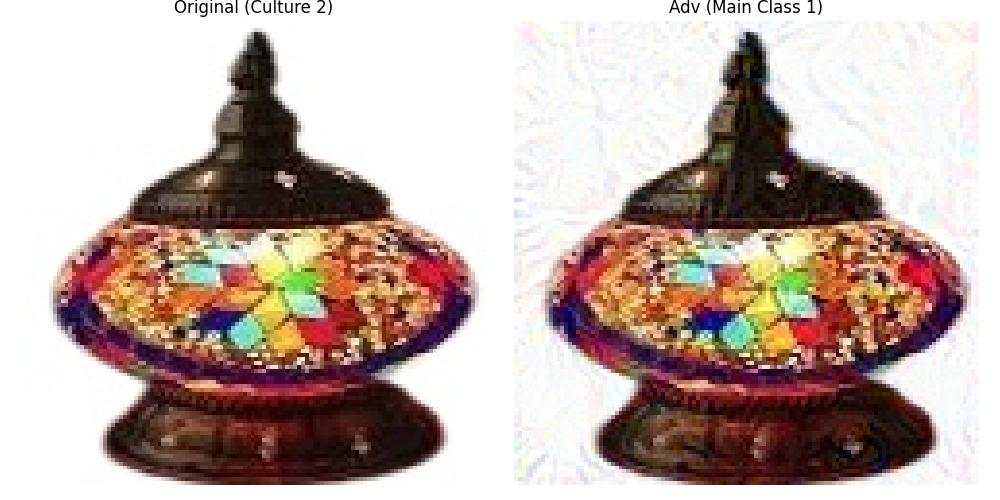
\includegraphics[width=\columnwidth]{adv_gen_figures/ADVmajLF_CLSDIV1_source_2.jpg}
\end{subfigure} 
\caption{Example of transformations applied on Chin., Fren. and Turk. images from LAMP dataset with lamps turned on using PGD and CLSDIV with Fren. as majority culture.}
\label{fig::advLF_CLSDIV1}
\end{figure}

\begin{figure}[H]
\centering
\begin{subfigure}[b]{0.6\columnwidth}
\centering
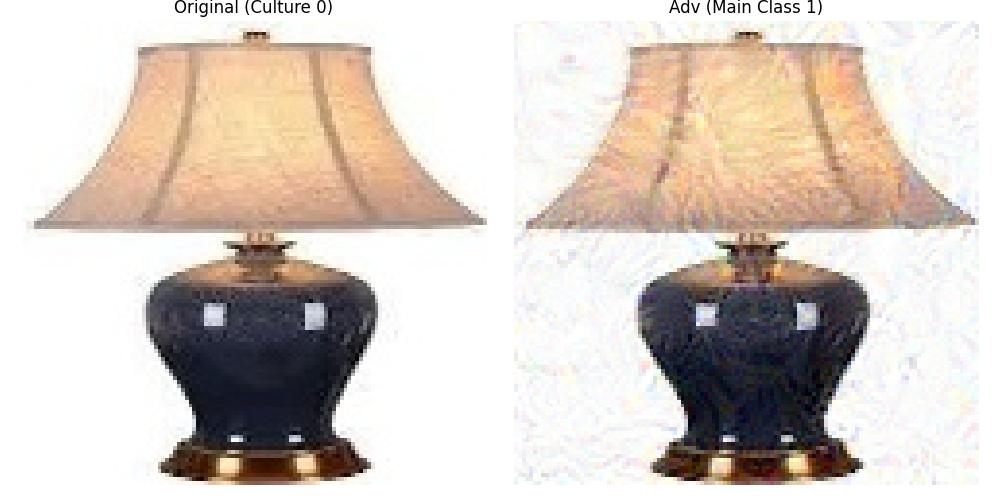
\includegraphics[width=\columnwidth]{adv_gen_figures/ADVmajLT_CLSDIV1_source_0.jpg}
\end{subfigure} \\
\begin{subfigure}[b]{0.6\columnwidth}
\centering
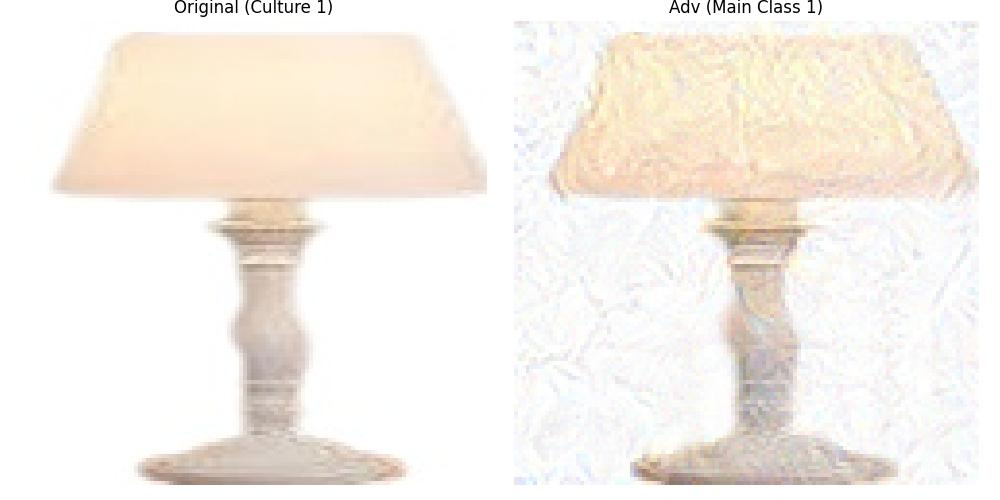
\includegraphics[width=\columnwidth]{adv_gen_figures/ADVmajLT_CLSDIV1_source_1.jpg}
\end{subfigure} \\
\begin{subfigure}[b]{0.6\columnwidth}
\centering
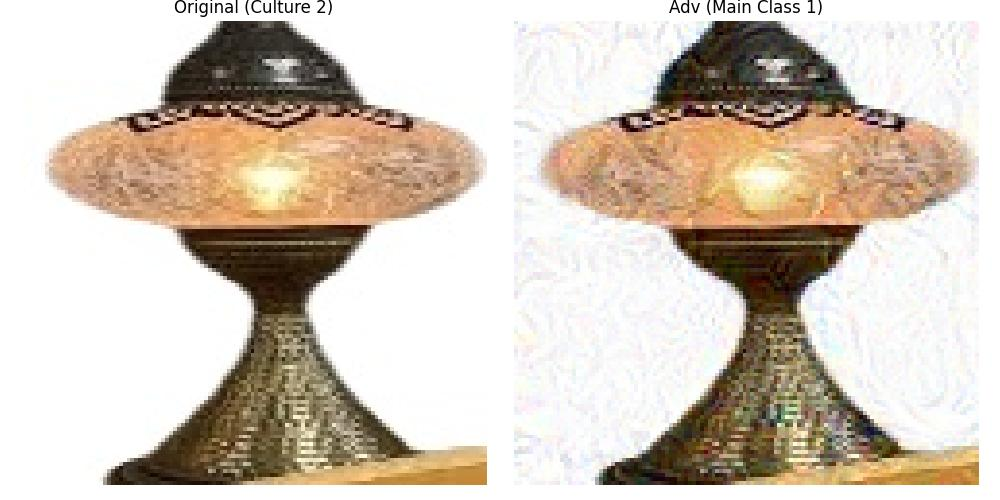
\includegraphics[width=\columnwidth]{adv_gen_figures/ADVmajLT_CLSDIV1_source_2.jpg}
\end{subfigure} 
\caption{Example of transformations applied on Chin., Fren. and Turk. images from LAMP dataset with lamps turned on using PGD and CLSDIV with Turk. as majority culture.}
\label{fig::advLT_CLSDIV1}
\end{figure}

% NOCLSDIV 0
\begin{figure}[H]
\centering
\begin{subfigure}[b]{0.6\columnwidth}
\centering
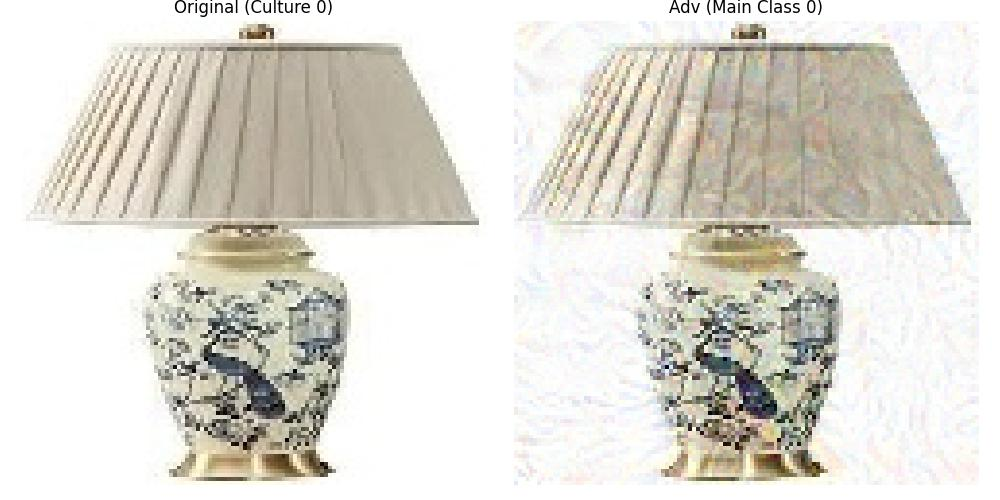
\includegraphics[width=\columnwidth]{adv_gen_figures/ADVmajLC_NOCLSDIV0_source_0.jpg}
\end{subfigure} \\
\begin{subfigure}[b]{0.6\columnwidth}
\centering
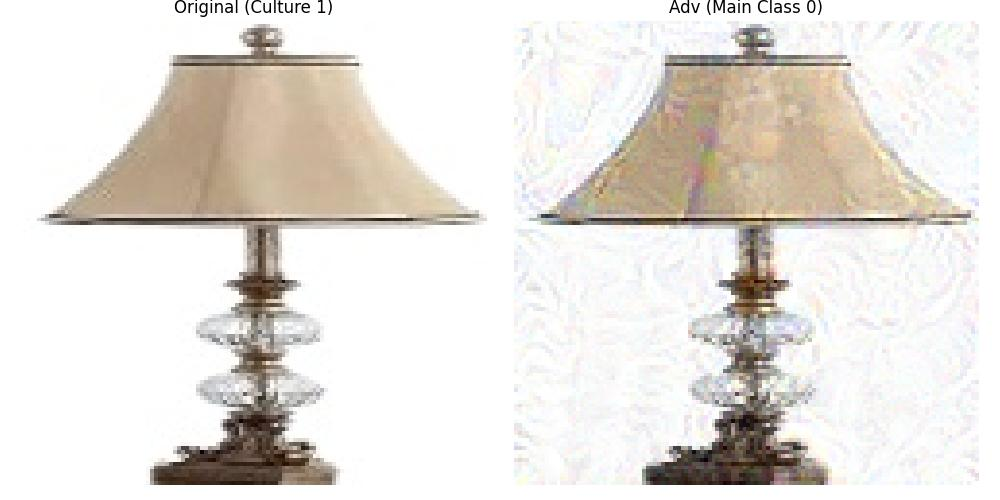
\includegraphics[width=\columnwidth]{adv_gen_figures/ADVmajLC_NOCLSDIV0_source_1.jpg}
\end{subfigure} \\
\begin{subfigure}[b]{0.6\columnwidth}
\centering
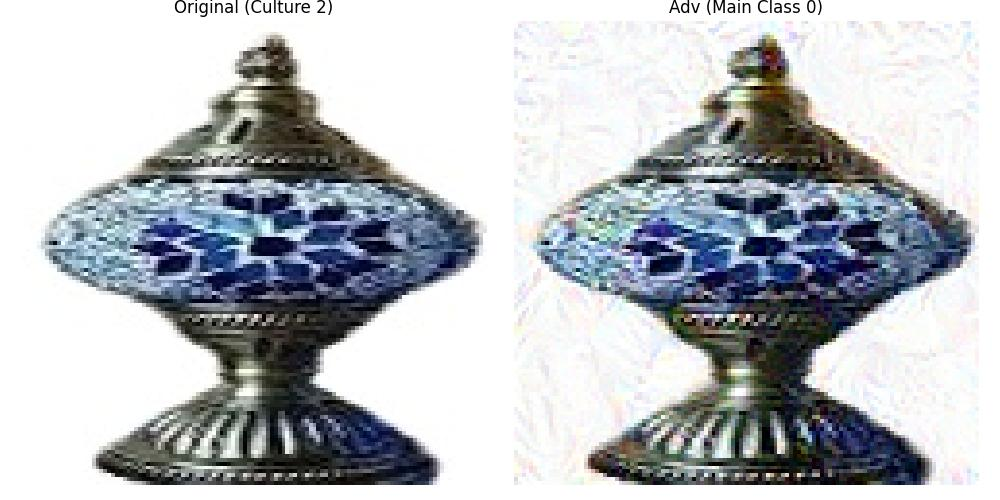
\includegraphics[width=\columnwidth]{adv_gen_figures/ADVmajLC_NOCLSDIV0_source_2.jpg}
\end{subfigure} 
\caption{Example of transformations applied on Chin., Fren. and Turk. images from LAMP dataset with lamps turned off using PGD and NOCLSDIV with Chin. as majority culture.}
\label{fig::advLC_NOCLSDIV0}
\end{figure}

\begin{figure}[H]
\centering
\begin{subfigure}[b]{0.6\columnwidth}
\centering
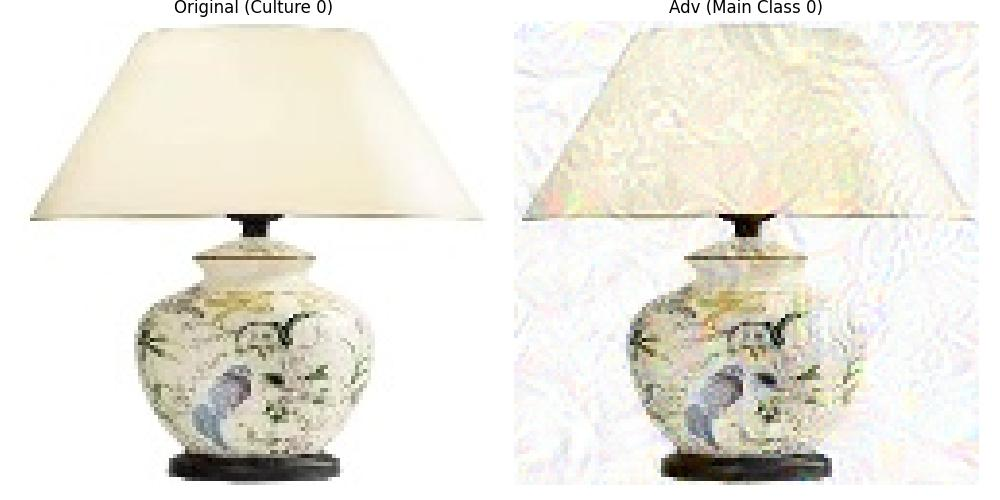
\includegraphics[width=\columnwidth]{adv_gen_figures/ADVmajLF_NOCLSDIV0_source_0.jpg}
\end{subfigure} \\
\begin{subfigure}[b]{0.6\columnwidth}
\centering
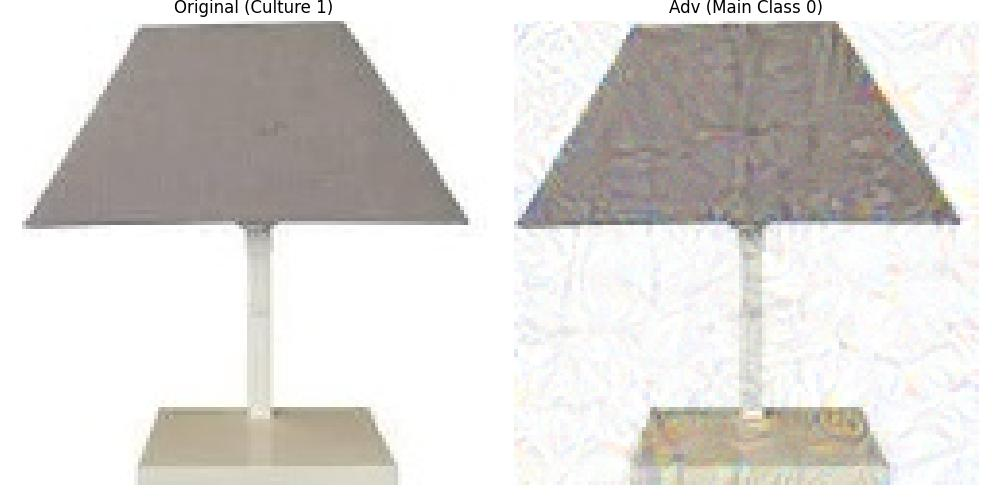
\includegraphics[width=\columnwidth]{adv_gen_figures/ADVmajLF_NOCLSDIV0_source_1.jpg}
\end{subfigure} \\
\begin{subfigure}[b]{0.6\columnwidth}
\centering
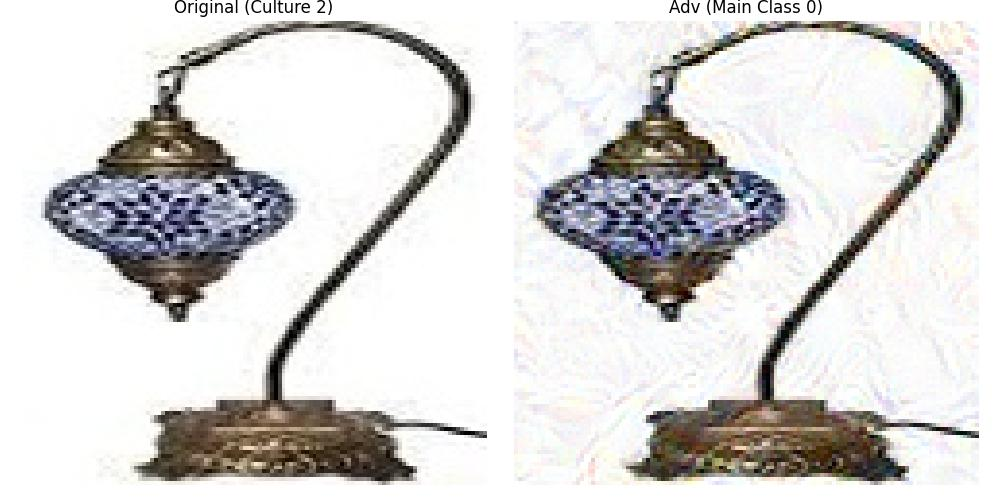
\includegraphics[width=\columnwidth]{adv_gen_figures/ADVmajLF_NOCLSDIV0_source_2.jpg}
\end{subfigure} 
\caption{Example of transformations applied on Chin., Fren. and Turk. images from LAMP dataset with lamps turned off using PGD and NOCLSDIV with Fren. as majority culture.}
\label{fig::advLF_NOCLSDIV0}
\end{figure}

\begin{figure}[H]
\centering
\begin{subfigure}[b]{0.6\columnwidth}
\centering
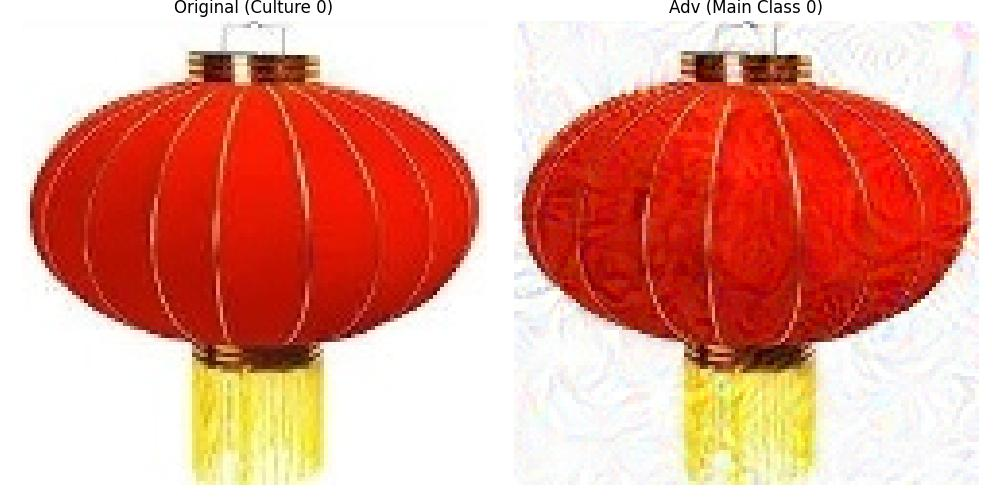
\includegraphics[width=\columnwidth]{adv_gen_figures/ADVmajLT_NOCLSDIV0_source_0.jpg}
\end{subfigure} \\
\begin{subfigure}[b]{0.6\columnwidth}
\centering
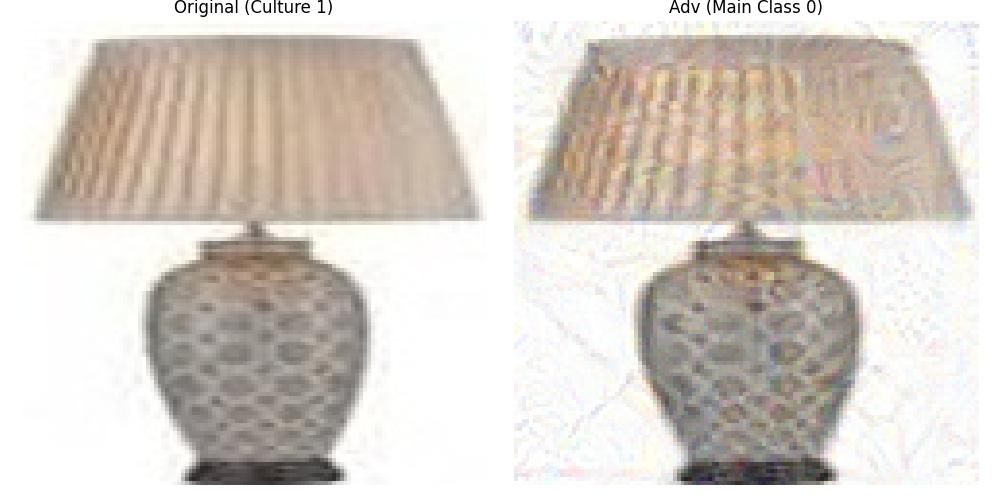
\includegraphics[width=\columnwidth]{adv_gen_figures/ADVmajLT_NOCLSDIV0_source_1.jpg}
\end{subfigure} \\
\begin{subfigure}[b]{0.6\columnwidth}
\centering
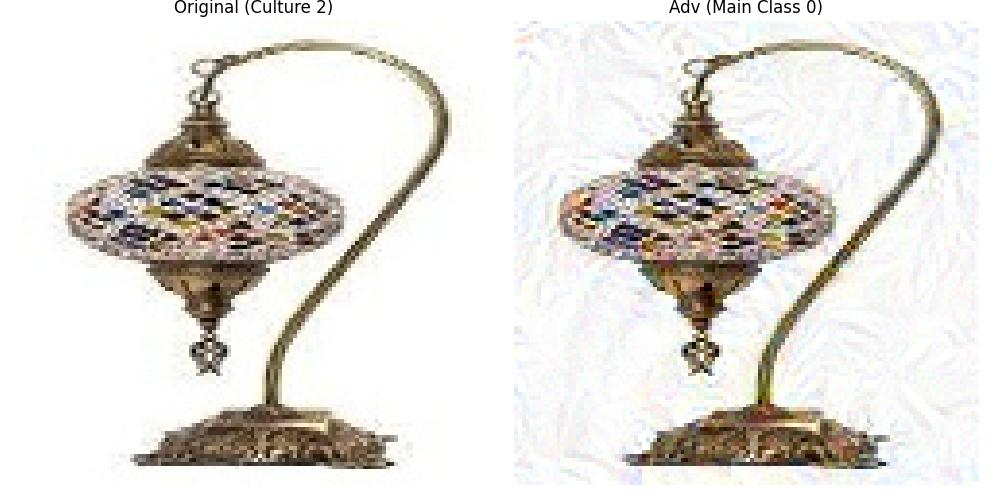
\includegraphics[width=\columnwidth]{adv_gen_figures/ADVmajLT_NOCLSDIV0_source_2.jpg}
\end{subfigure} 
\caption{Example of transformations applied on Chin., Fren. and Turk. images from LAMP dataset with lamps turned off using PGD and NOCLSDIV with Turk. as majority culture.}
\label{fig::advLT_NOCLSDIV0}
\end{figure}

% NOCLSDIV 1
\begin{figure}[H]
\centering
\begin{subfigure}[b]{0.6\columnwidth}
\centering
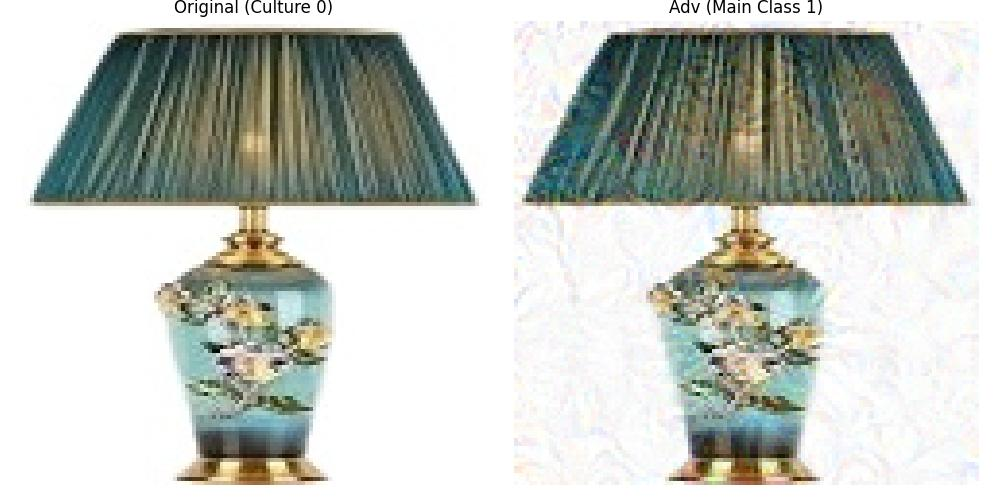
\includegraphics[width=\columnwidth]{adv_gen_figures/ADVmajLC_NOCLSDIV1_source_0.jpg}
\end{subfigure} \\
\begin{subfigure}[b]{0.6\columnwidth}
\centering
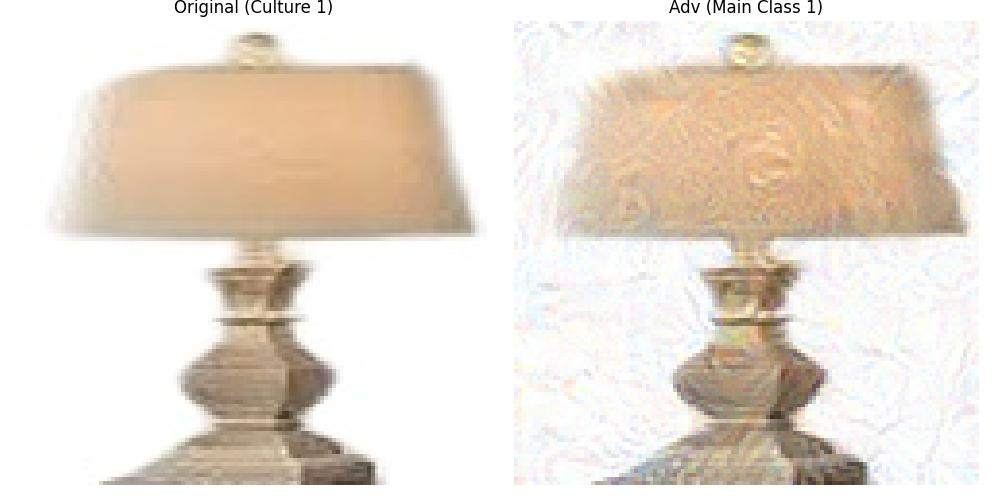
\includegraphics[width=\columnwidth]{adv_gen_figures/ADVmajLC_NOCLSDIV1_source_1.jpg}
\end{subfigure} \\
\begin{subfigure}[b]{0.6\columnwidth}
\centering
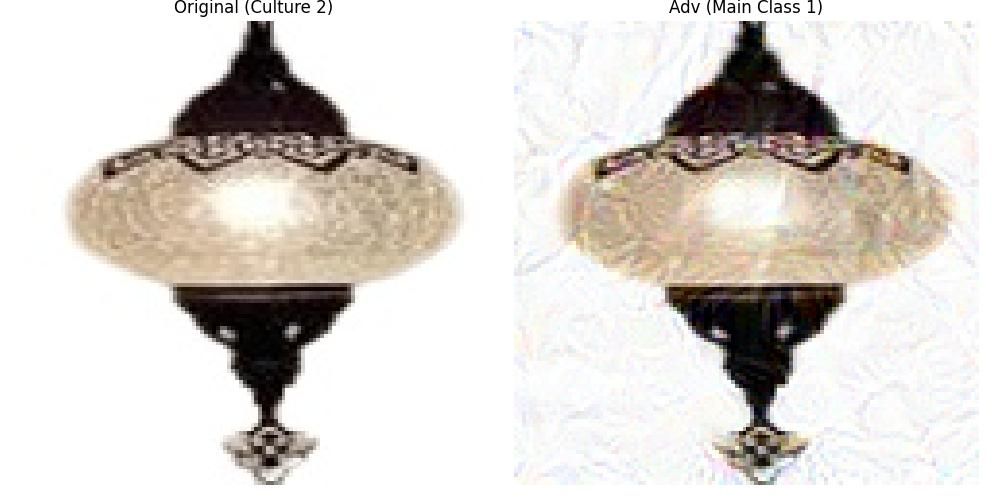
\includegraphics[width=\columnwidth]{adv_gen_figures/ADVmajLC_NOCLSDIV1_source_2.jpg}
\end{subfigure} 
\caption{Example of transformations applied on Chin., Fren. and Turk. images from LAMP dataset with lamps turned on using PGD and NOCLSDIV with Chin. as majority culture.}
\label{fig::advLC_NOCLSDIV1}
\end{figure}

\begin{figure}[H]
\centering
\begin{subfigure}[b]{0.6\columnwidth}
\centering
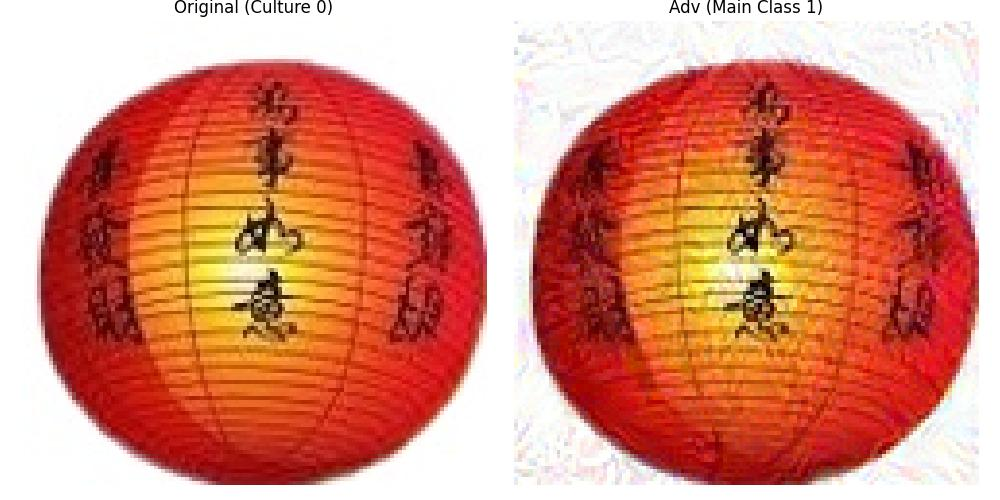
\includegraphics[width=\columnwidth]{adv_gen_figures/ADVmajLF_NOCLSDIV1_source_0.jpg}
\end{subfigure} \\
\begin{subfigure}[b]{0.6\columnwidth}
\centering
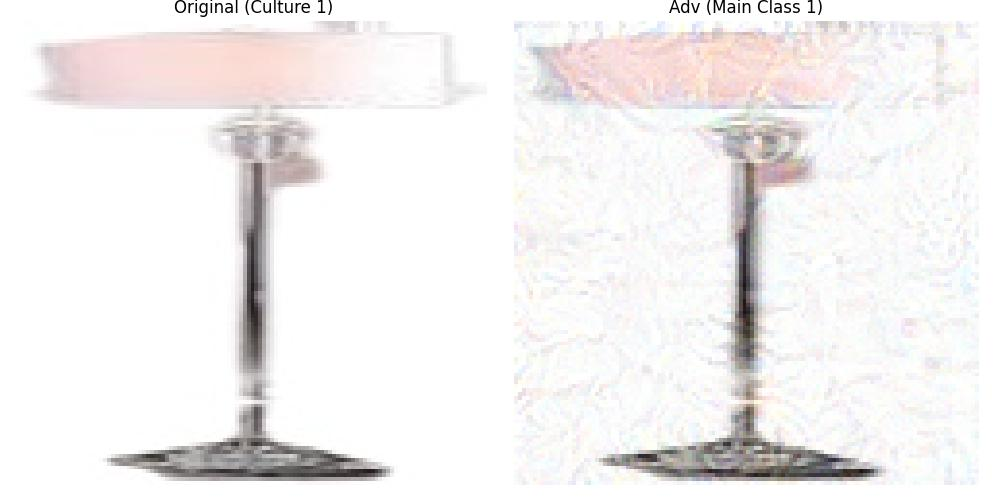
\includegraphics[width=\columnwidth]{adv_gen_figures/ADVmajLF_NOCLSDIV1_source_1.jpg}
\end{subfigure} \\
\begin{subfigure}[b]{0.6\columnwidth}
\centering
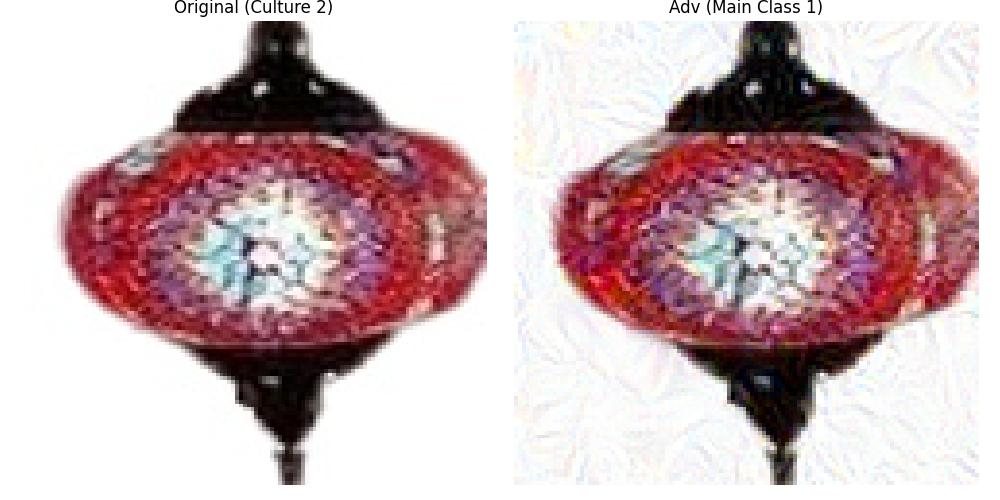
\includegraphics[width=\columnwidth]{adv_gen_figures/ADVmajLF_NOCLSDIV1_source_2.jpg}
\end{subfigure} 
\caption{Example of transformations applied on Chin., Fren. and Turk. images from LAMP dataset with lamps turned on using PGD and NOCLSDIV with Fren. as majority culture.}
\label{fig::advLF_NOCLSDIV1}
\end{figure}

\begin{figure}[H]
\centering
\begin{subfigure}[b]{0.6\columnwidth}
\centering
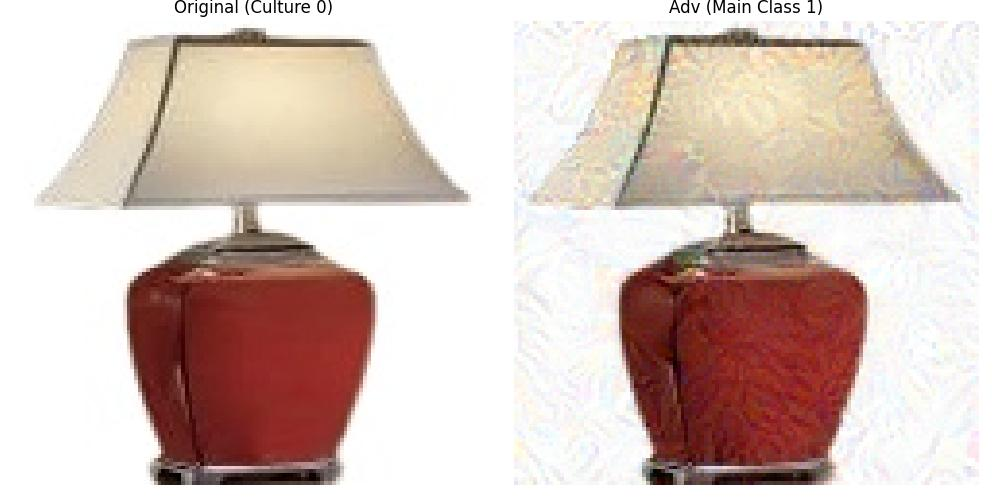
\includegraphics[width=\columnwidth]{adv_gen_figures/ADVmajLT_NOCLSDIV1_source_0.jpg}
\end{subfigure} \\
\begin{subfigure}[b]{0.6\columnwidth}
\centering
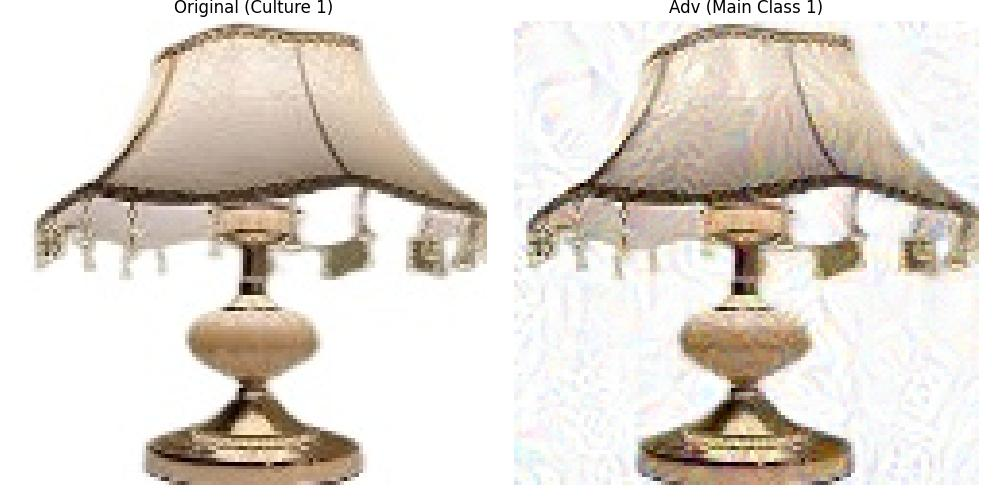
\includegraphics[width=\columnwidth]{adv_gen_figures/ADVmajLT_NOCLSDIV1_source_1.jpg}
\end{subfigure} \\
\begin{subfigure}[b]{0.6\columnwidth}
\centering
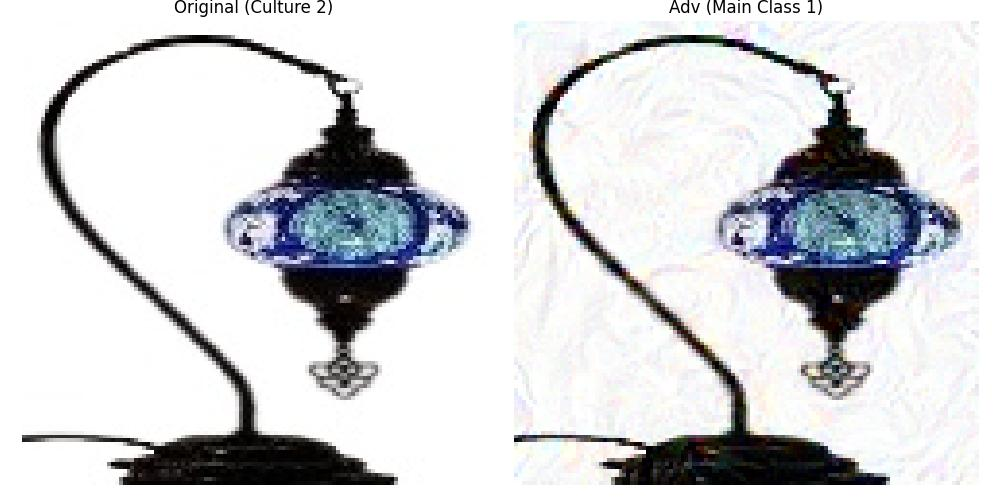
\includegraphics[width=\columnwidth]{adv_gen_figures/ADVmajLT_NOCLSDIV1_source_2.jpg}
\end{subfigure} 
\caption{Example of transformations applied on Chin., Fren. and Turk. images from LAMP dataset with lamps turned on using PGD and NOCLSDIV with Turk. as majority culture.}
\label{fig::advLT_NOCLSDIV1}
\end{figure}
Tables~\ref{fig::advCI_CLSDIV0}, \ref{fig::advCI_CLSDIV1}, \ref{fig::advCI_NOCLSDIV0}, \ref{fig::advCI_NOCLSDIV1}, \ref{fig::advCJ_CLSDIV0}, \ref{fig::advCJ_CLSDIV1}, \ref{fig::advCJ_NOCLSDIV0}, \ref{fig::advCJ_NOCLSDIV1},
\ref{fig::advCS_CLSDIV0}, \ref{fig::advCS_CLSDIV1}, \ref{fig::advCS_NOCLSDIV0}, \ref{fig::advCS_NOCLSDIV1} show examples of transformations applied on Ind., Jap., and Scan. images from CARPET dataset with lamps turned off using PGD and CLSDIV or NOCLSDIV with Ind., Jap., and Scan. as majority cultures.
% CARPET
\begin{figure}[H]
\centering
\begin{subfigure}[b]{0.6\columnwidth}
\centering
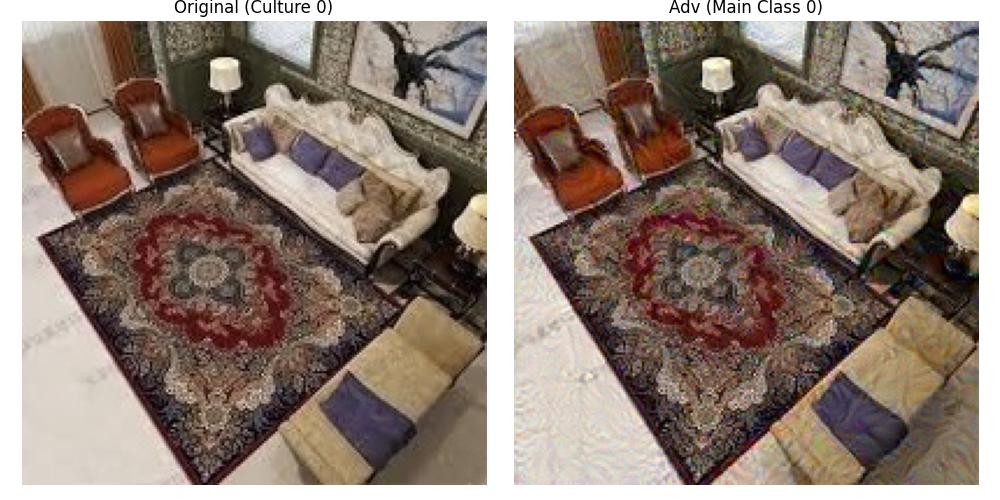
\includegraphics[width=\columnwidth]{adv_gen_figures/ADVmajCI_CLSDIV0_source_0.jpg}
\end{subfigure} \\
\begin{subfigure}[b]{0.6\columnwidth}
\centering
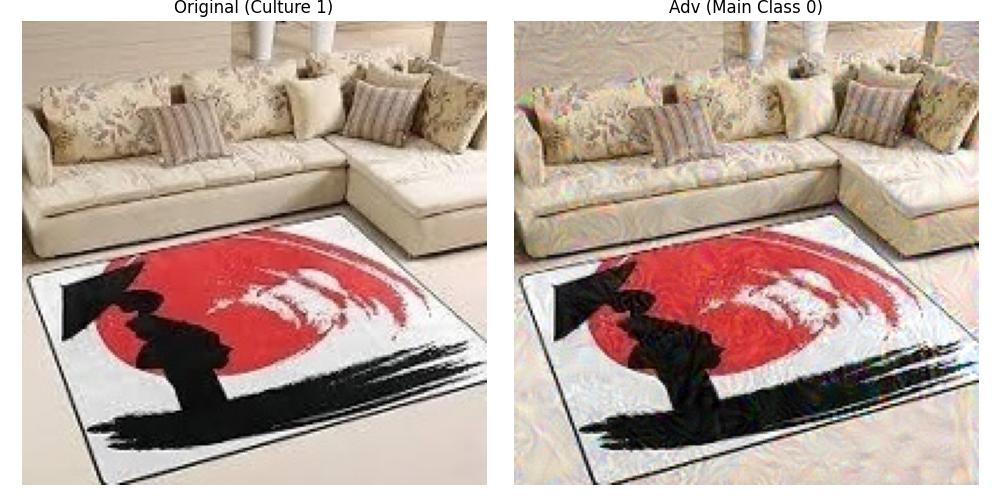
\includegraphics[width=\columnwidth]{adv_gen_figures/ADVmajCI_CLSDIV0_source_1.jpg}
\end{subfigure} \\
\begin{subfigure}[b]{0.6\columnwidth}
\centering
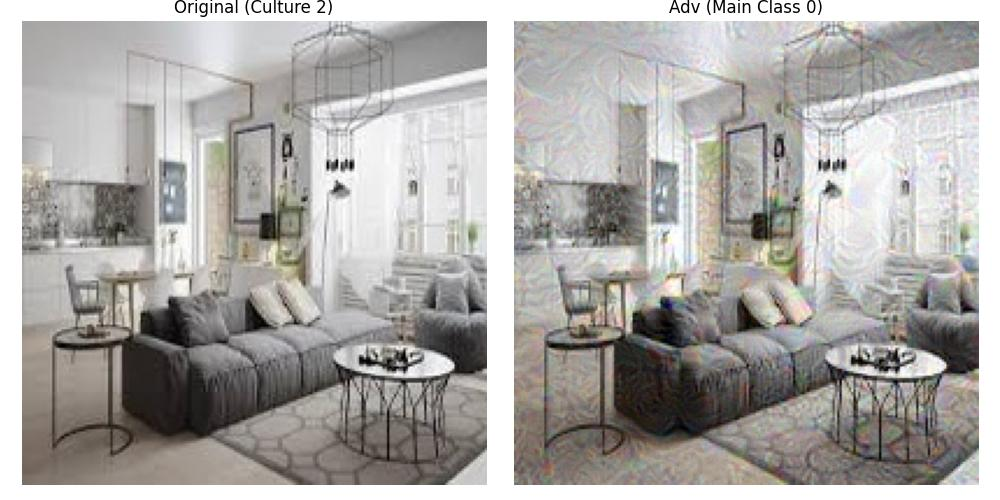
\includegraphics[width=\columnwidth]{adv_gen_figures/ADVmajCI_CLSDIV0_source_2.jpg}
\end{subfigure} 
\caption{Example of transformations applied on Ind. Jap. and Scan. dataset with with carpets using PGD and CLSDIV with Ind. as majority culture.}
\label{fig::advCI_CLSDIV0}
\end{figure}

\begin{figure}[H]
\centering
\begin{subfigure}[b]{0.6\columnwidth}
\centering
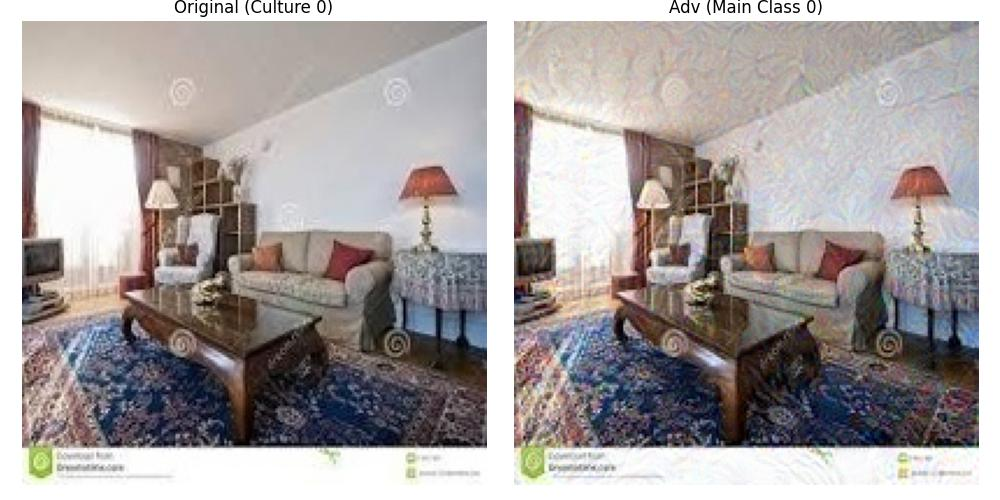
\includegraphics[width=\columnwidth]{adv_gen_figures/ADVmajCJ_CLSDIV0_source_0.jpg}

\end{subfigure} \\
\begin{subfigure}[b]{0.6\columnwidth}
\centering
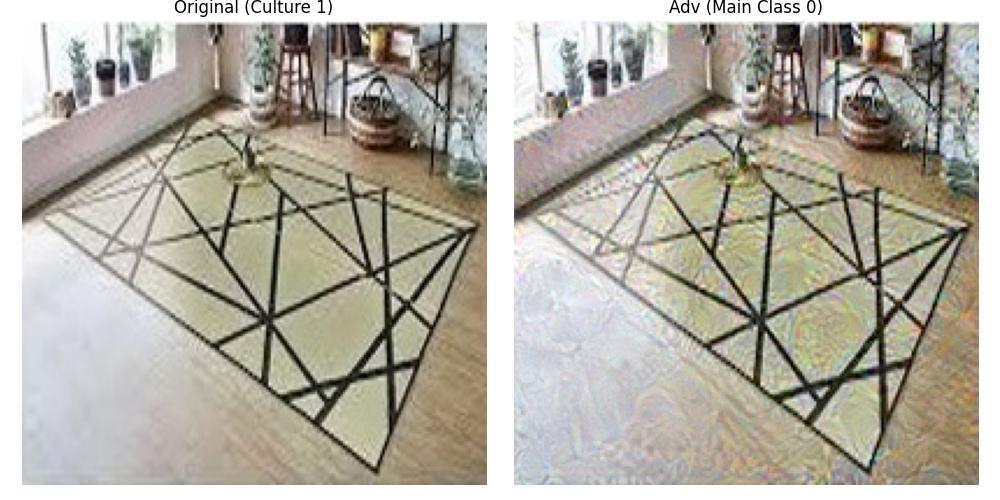
\includegraphics[width=\columnwidth]{adv_gen_figures/ADVmajCJ_CLSDIV0_source_1.jpg}
\end{subfigure} \\
\begin{subfigure}[b]{0.6\columnwidth}
\centering
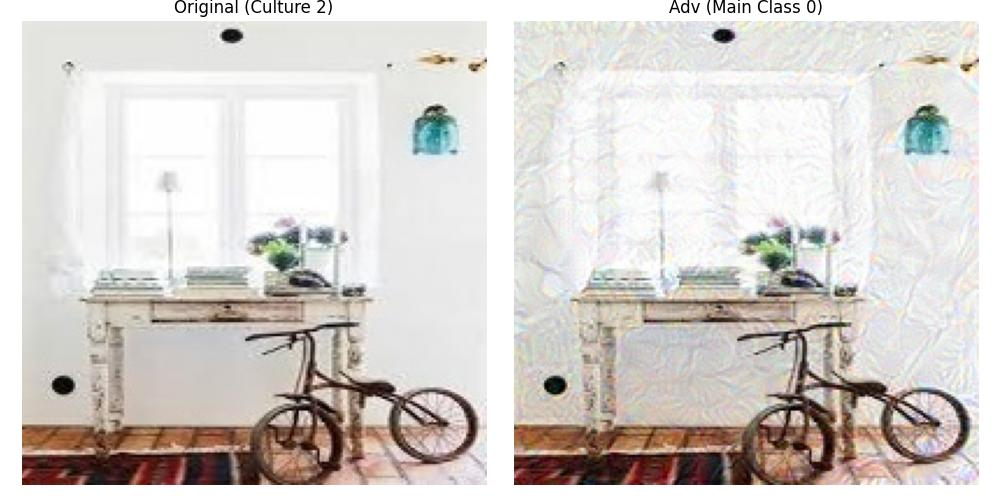
\includegraphics[width=\columnwidth]{adv_gen_figures/ADVmajCJ_CLSDIV0_source_2.jpg}
\end{subfigure} 
\caption{Example of transformations applied on Ind. Jap. and Scan. dataset with with carpets using PGD and CLSDIV with Jap. as majority culture.}
\label{fig::advCJ_CLSDIV0}
\end{figure}

\begin{figure}[H]
\centering
\begin{subfigure}[b]{0.6\columnwidth}
\centering
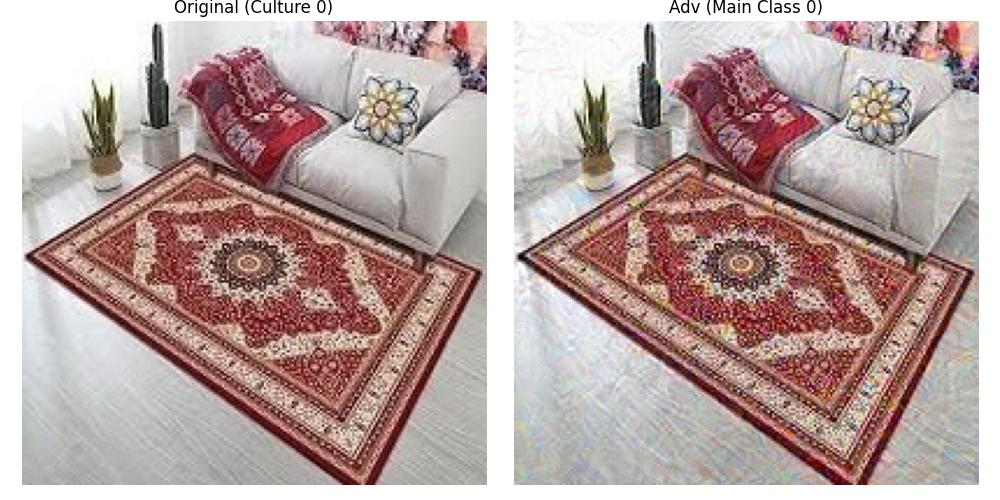
\includegraphics[width=\columnwidth]{adv_gen_figures/ADVmajCS_CLSDIV0_source_0.jpg}
\end{subfigure} \\
\begin{subfigure}[b]{0.6\columnwidth}
\centering
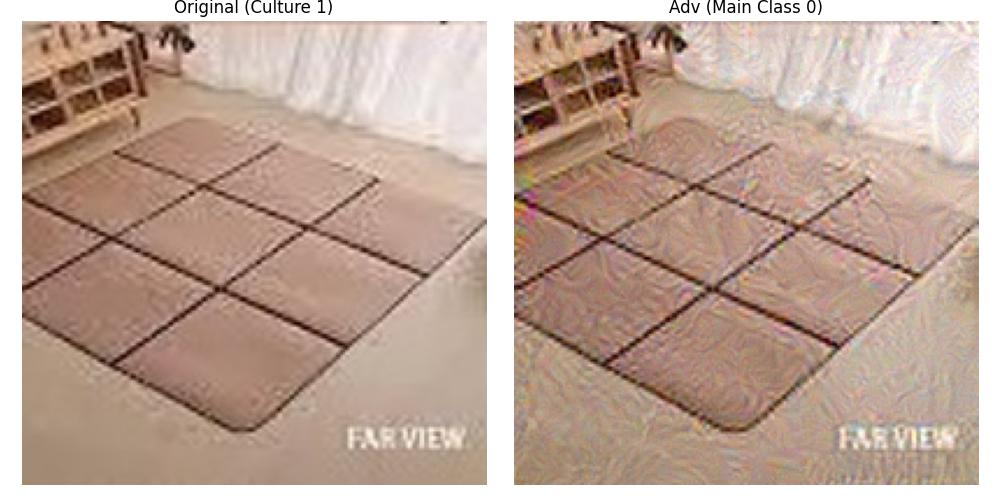
\includegraphics[width=\columnwidth]{adv_gen_figures/ADVmajCS_CLSDIV0_source_1.jpg}
\end{subfigure} \\
\begin{subfigure}[b]{0.6\columnwidth}
\centering
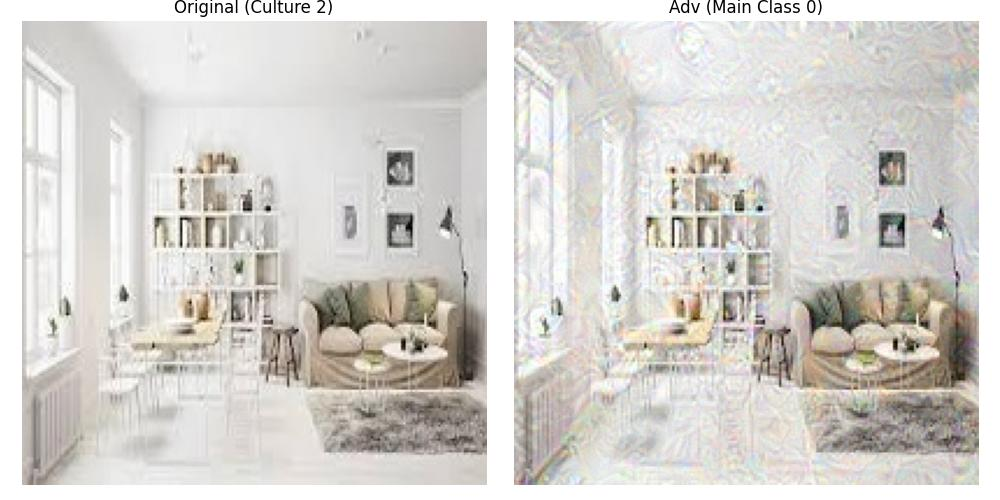
\includegraphics[width=\columnwidth]{adv_gen_figures/ADVmajCS_CLSDIV0_source_2.jpg}
\end{subfigure} 
\caption{Example of transformations applied on Ind. Jap. and Scan. dataset with with carpets using PGD and CLSDIV with Scan. as majority culture.}
\label{fig::advCS_CLSDIV0}
\end{figure}

%CLSDIV 1
\begin{figure}[H]
\centering
\begin{subfigure}[b]{0.6\columnwidth}
\centering
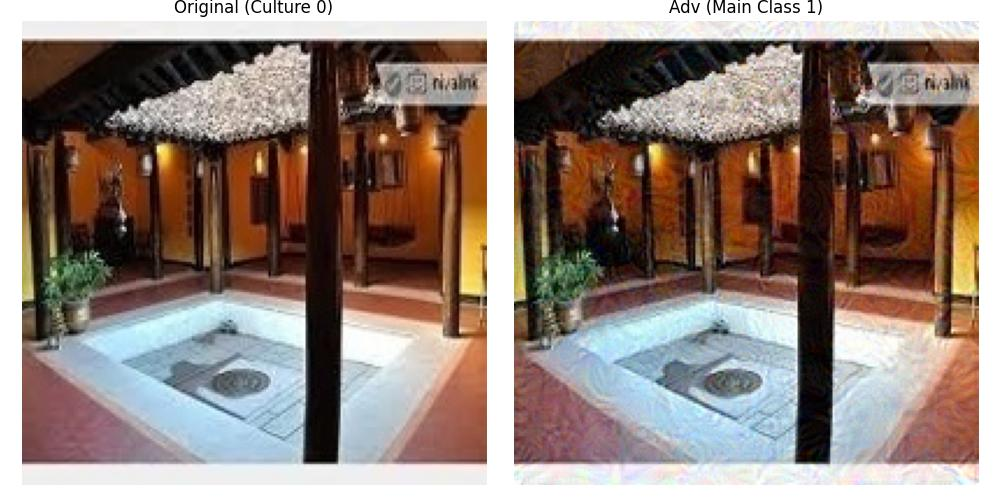
\includegraphics[width=\columnwidth]{adv_gen_figures/ADVmajCI_CLSDIV1_source_0.jpg}
\end{subfigure} \\
\begin{subfigure}[b]{0.6\columnwidth}
\centering
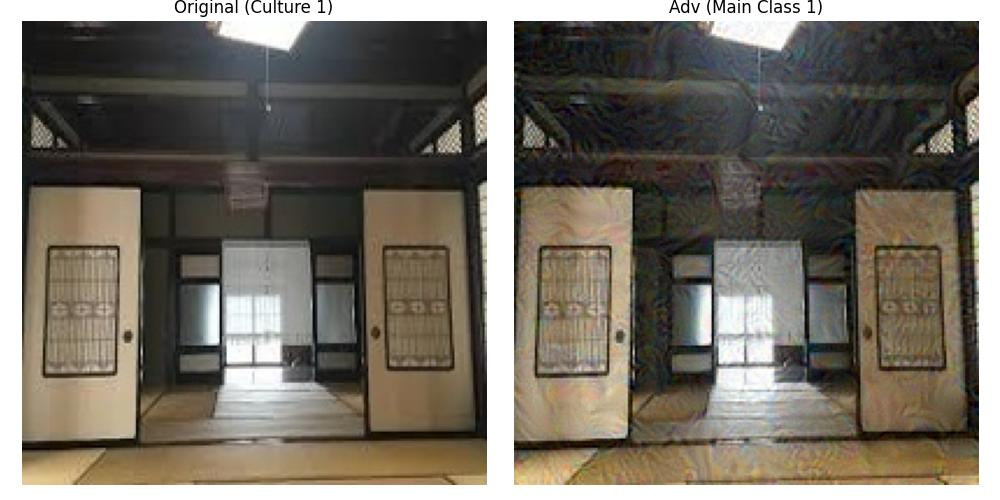
\includegraphics[width=\columnwidth]{adv_gen_figures/ADVmajCI_CLSDIV1_source_1.jpg}
\end{subfigure} \\
\begin{subfigure}[b]{0.6\columnwidth}
\centering
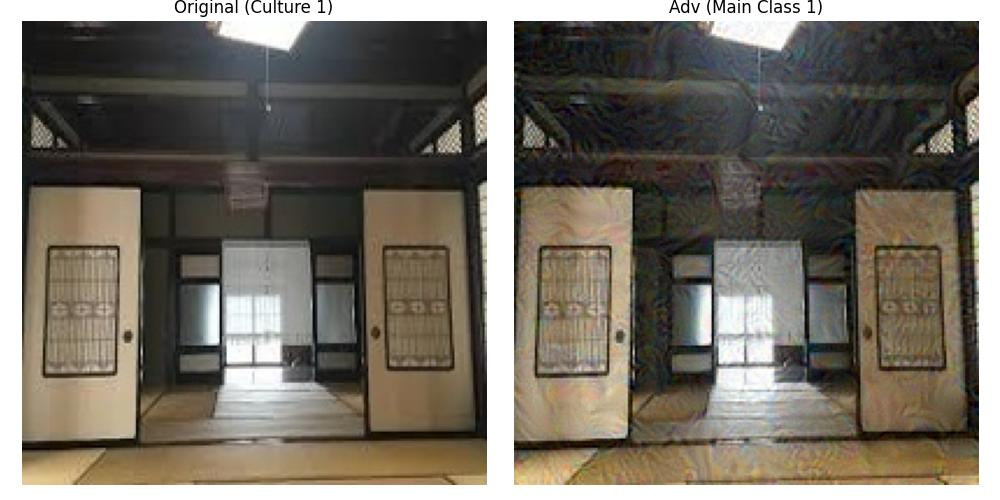
\includegraphics[width=\columnwidth]{adv_gen_figures/ADVmajCI_CLSDIV1_source_2.jpg}
\end{subfigure} 
\caption{Example of transformations applied on Ind. Jap. and Scan. dataset without carpets using PGD and CLSDIV with Ind. as majority culture.}
\label{fig::advCI_CLSDIV1}
\end{figure}

\begin{figure}[H]
\centering
\begin{subfigure}[b]{0.6\columnwidth}
\centering
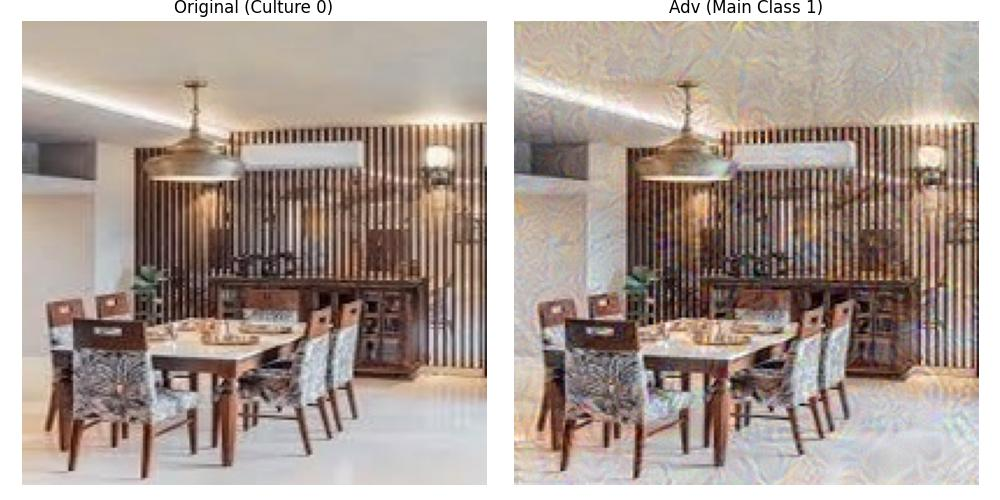
\includegraphics[width=\columnwidth]{adv_gen_figures/ADVmajCJ_CLSDIV1_source_0.jpg}
\end{subfigure} \\
\begin{subfigure}[b]{0.6\columnwidth}
\centering
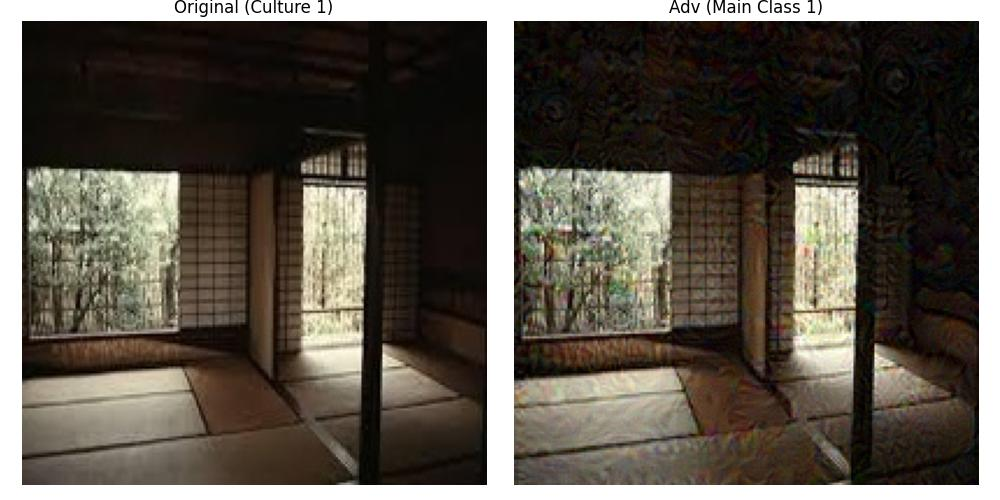
\includegraphics[width=\columnwidth]{adv_gen_figures/ADVmajCJ_CLSDIV1_source_1.jpg}
\end{subfigure} \\
\begin{subfigure}[b]{0.6\columnwidth}
\centering
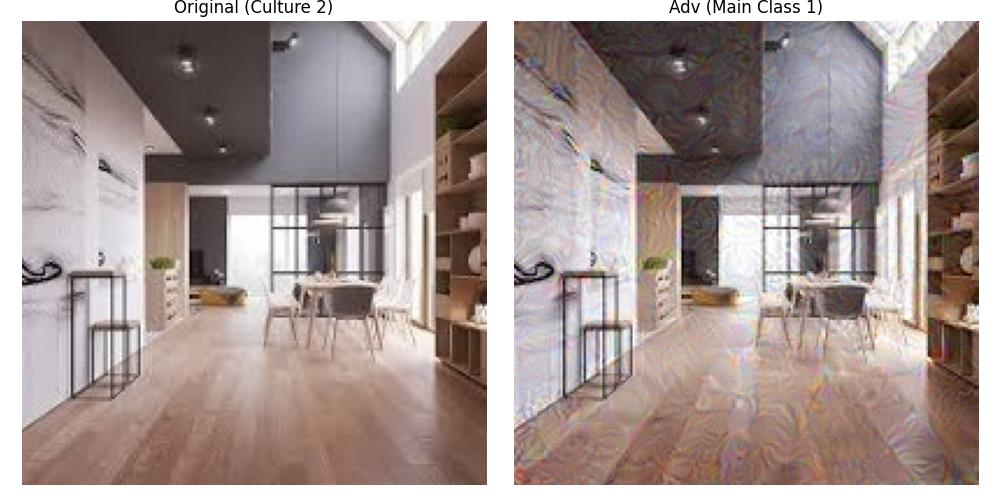
\includegraphics[width=\columnwidth]{adv_gen_figures/ADVmajCJ_CLSDIV1_source_2.jpg}
\end{subfigure} 
\caption{Example of transformations applied on Ind. Jap. and Scan. dataset without carpets using PGD and CLSDIV with Jap. as majority culture.}
\label{fig::advCJ_CLSDIV1}
\end{figure}

\begin{figure}[H]
\centering
\begin{subfigure}[b]{0.6\columnwidth}
\centering
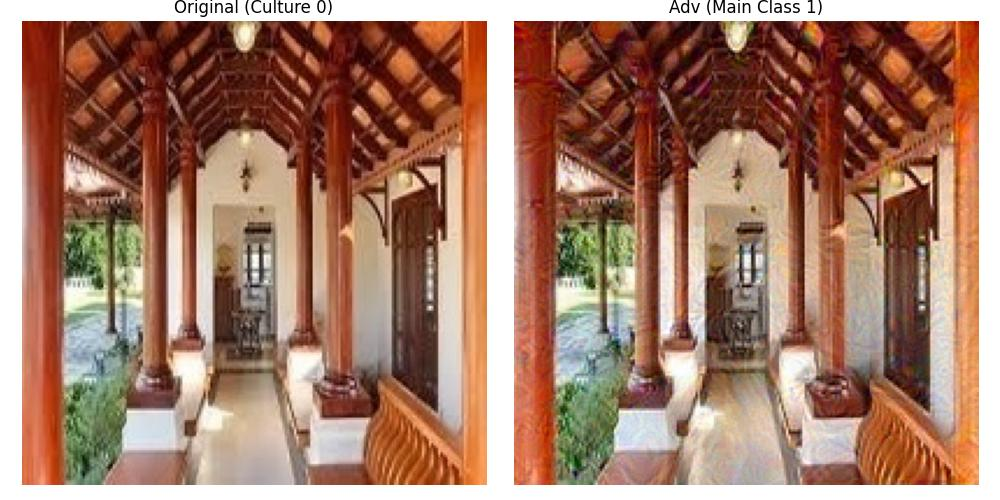
\includegraphics[width=\columnwidth]{adv_gen_figures/ADVmajCS_CLSDIV1_source_0.jpg}
\end{subfigure} \\
\begin{subfigure}[b]{0.6\columnwidth}
\centering
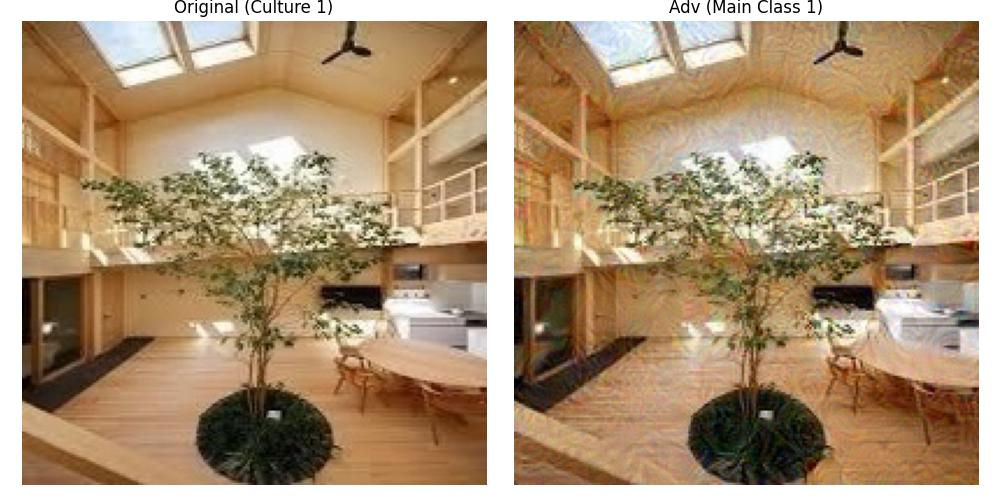
\includegraphics[width=\columnwidth]{adv_gen_figures/ADVmajCS_CLSDIV1_source_1.jpg}
\end{subfigure} \\
\begin{subfigure}[b]{0.6\columnwidth}
\centering
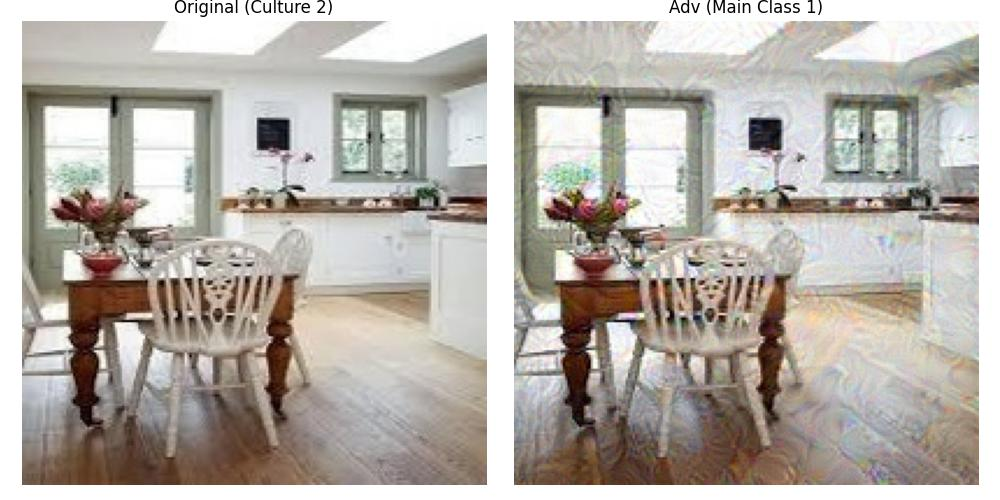
\includegraphics[width=\columnwidth]{adv_gen_figures/ADVmajCS_CLSDIV1_source_2.jpg}
\end{subfigure} 
\caption{Example of transformations applied on Ind. Jap. and Scan. dataset without carpets using PGD and CLSDIV with Scan. as majority culture.}
\label{fig::advCS_CLSDIV1}
\end{figure}

% NOCLSDIV 0
\begin{figure}[H]
\centering
\begin{subfigure}[b]{0.6\columnwidth}
\centering
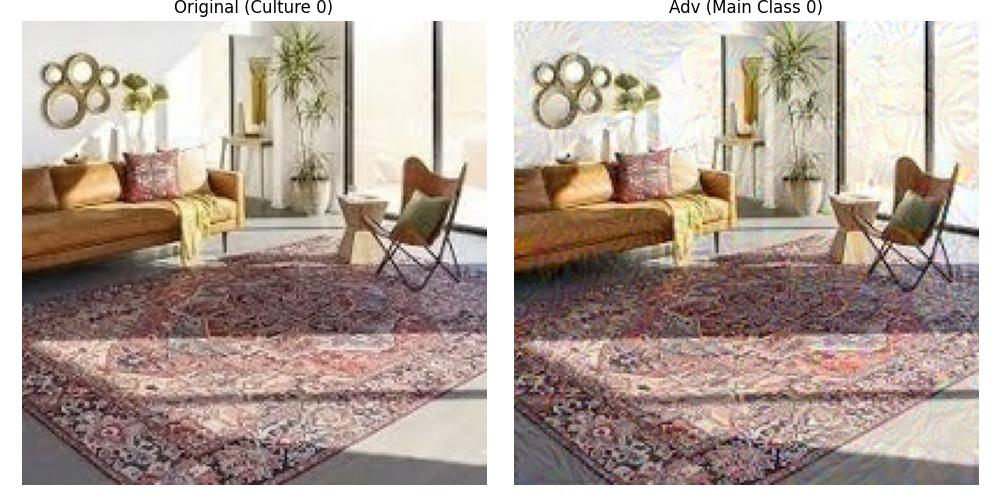
\includegraphics[width=\columnwidth]{adv_gen_figures/ADVmajCI_NOCLSDIV0_source_0.jpg}
\end{subfigure} \\
\begin{subfigure}[b]{0.6\columnwidth}
\centering
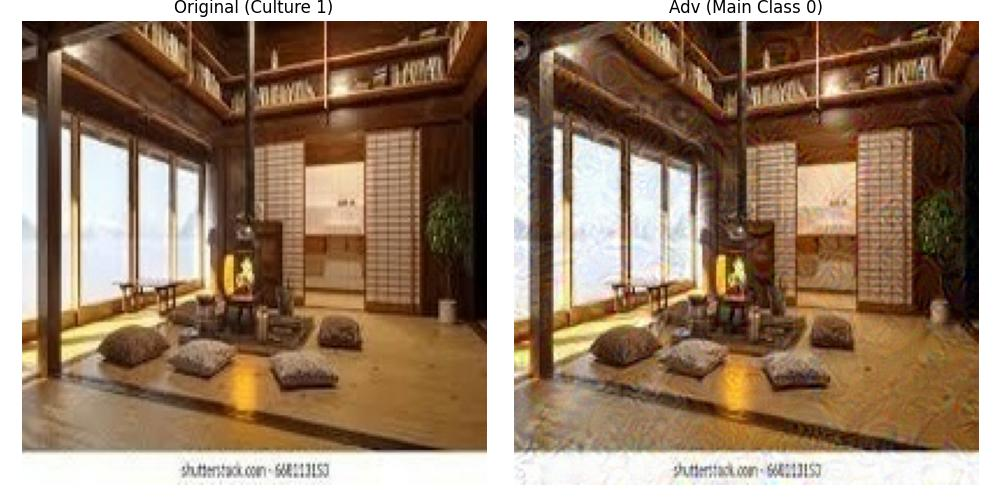
\includegraphics[width=\columnwidth]{adv_gen_figures/ADVmajCI_NOCLSDIV0_source_1.jpg}
\end{subfigure} \\
\begin{subfigure}[b]{0.6\columnwidth}
\centering
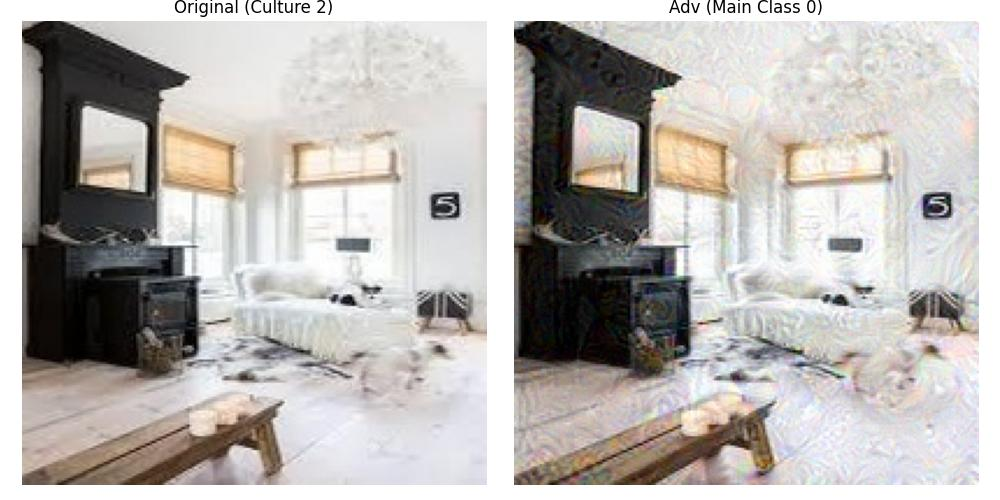
\includegraphics[width=\columnwidth]{adv_gen_figures/ADVmajCI_NOCLSDIV0_source_2.jpg}
\end{subfigure} 
\caption{Example of transformations applied on Ind. Jap. and Scan. dataset with with carpets using PGD and NOCLSDIV with Ind. as majority culture.}
\label{fig::advCI_NOCLSDIV0}
\end{figure}

\begin{figure}[H]
\centering
\begin{subfigure}[b]{0.6\columnwidth}
\centering
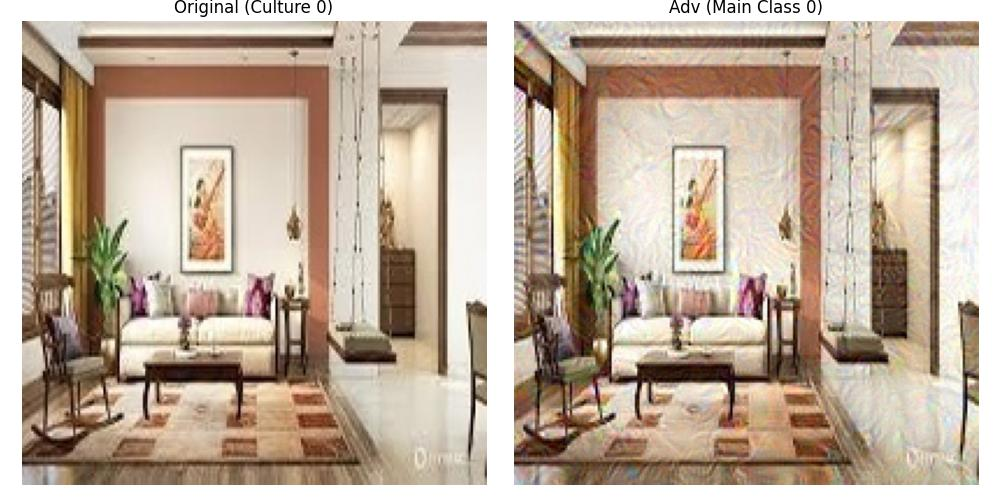
\includegraphics[width=\columnwidth]{adv_gen_figures/ADVmajCJ_NOCLSDIV0_source_0.jpg}
\end{subfigure} \\
\begin{subfigure}[b]{0.6\columnwidth}
\centering
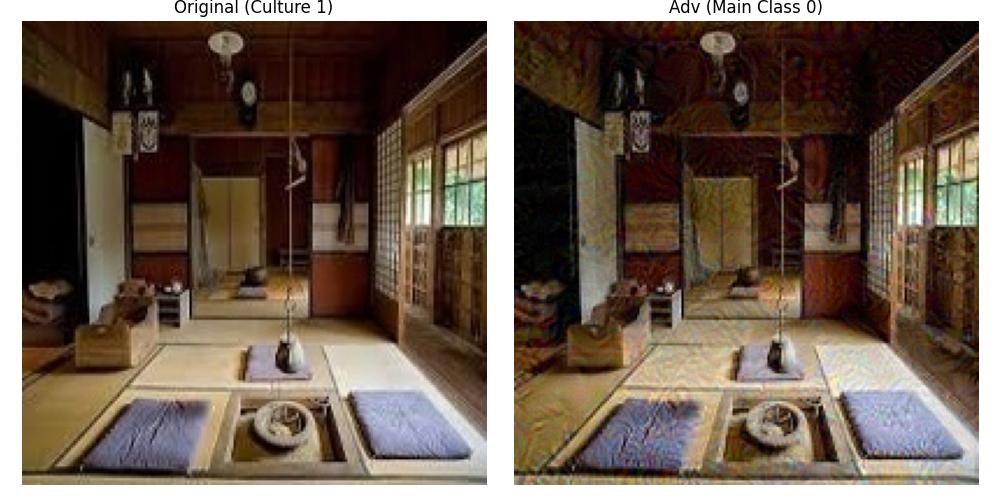
\includegraphics[width=\columnwidth]{adv_gen_figures/ADVmajCJ_NOCLSDIV0_source_1.jpg}
\end{subfigure} \\
\begin{subfigure}[b]{0.6\columnwidth}
\centering
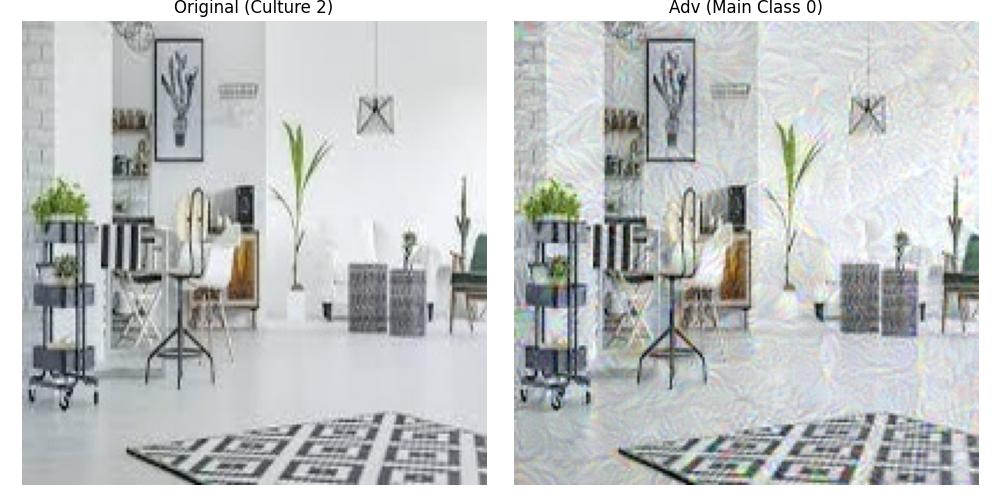
\includegraphics[width=\columnwidth]{adv_gen_figures/ADVmajCJ_NOCLSDIV0_source_2.jpg}
\end{subfigure} 
\caption{Example of transformations applied on Ind. Jap. and Scan. dataset with with carpets using PGD and NOCLSDIV with Jap. as majority culture.}
\label{fig::advCJ_NOCLSDIV0}
\end{figure}

\begin{figure}[H]
\centering
\begin{subfigure}[b]{0.6\columnwidth}
\centering
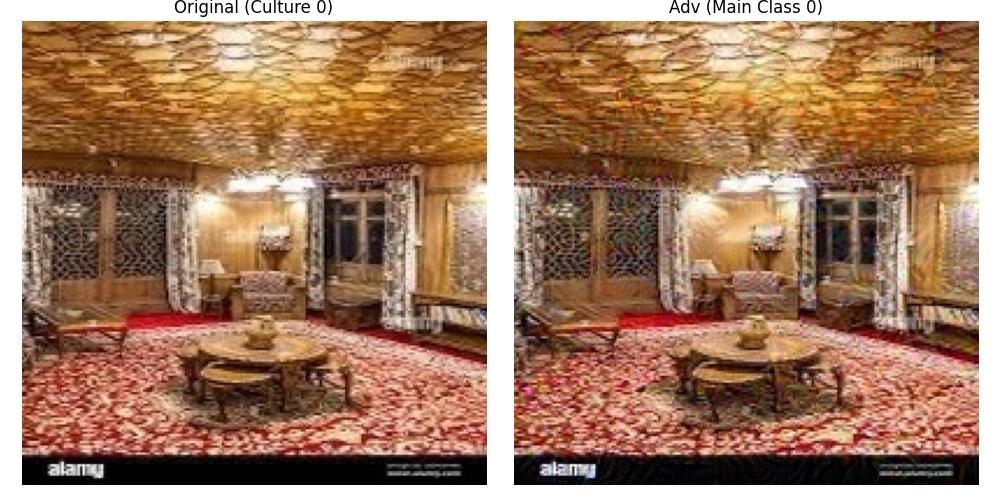
\includegraphics[width=\columnwidth]{adv_gen_figures/ADVmajCS_NOCLSDIV0_source_0.jpg}
\end{subfigure} \\
\begin{subfigure}[b]{0.6\columnwidth}
\centering
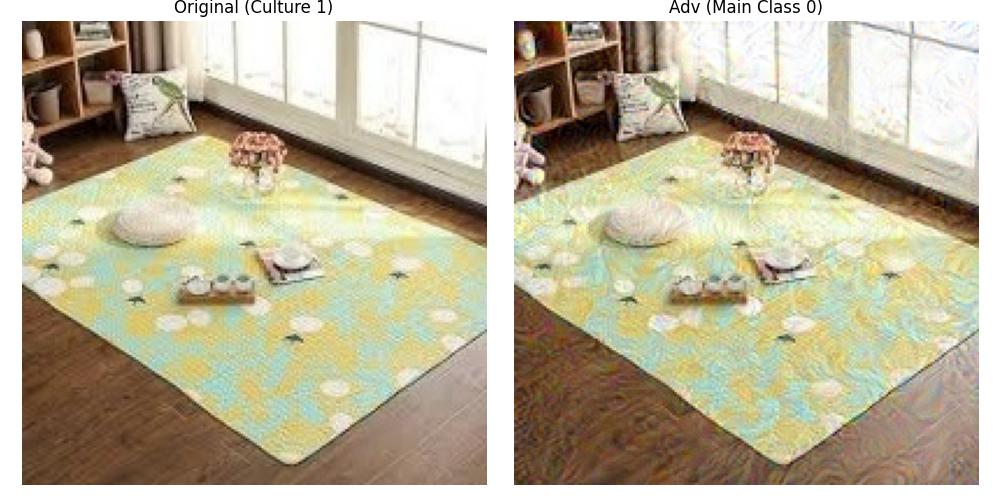
\includegraphics[width=\columnwidth]{adv_gen_figures/ADVmajCS_NOCLSDIV0_source_1.jpg}
\end{subfigure} \\
\begin{subfigure}[b]{0.6\columnwidth}
\centering
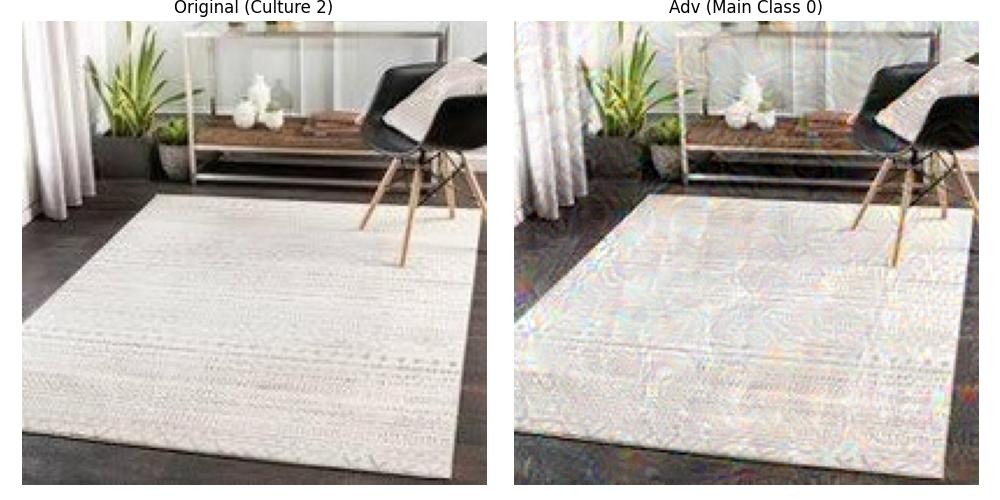
\includegraphics[width=\columnwidth]{adv_gen_figures/ADVmajCS_NOCLSDIV0_source_2.jpg}
\end{subfigure} 
\caption{Example of transformations applied on Ind. Jap. and Scan. dataset with with carpets using PGD and NOCLSDIV with Scan. as majority culture.}
\label{fig::advCS_NOCLSDIV0}
\end{figure}

% NOCLSDIV 1
\begin{figure}[H]
\centering
\begin{subfigure}[b]{0.6\columnwidth}
\centering
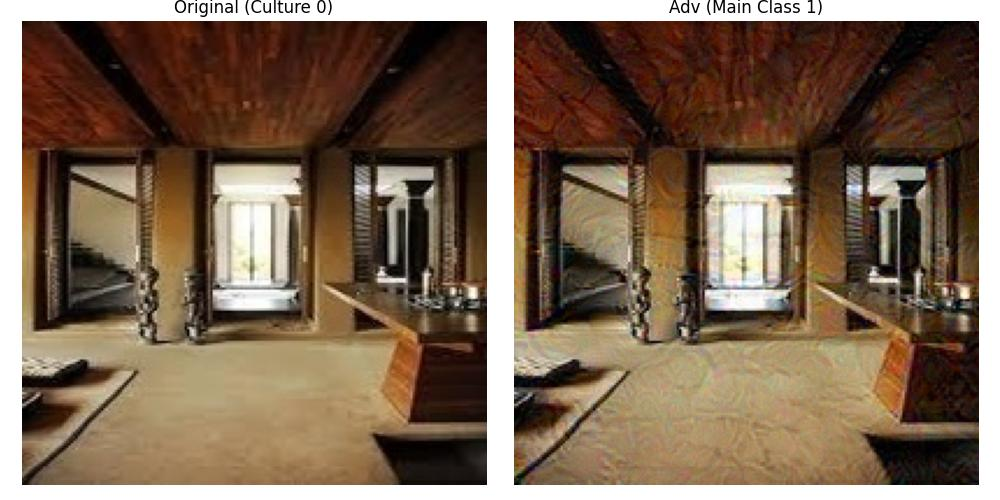
\includegraphics[width=\columnwidth]{adv_gen_figures/ADVmajCI_NOCLSDIV1_source_0.jpg}
\end{subfigure} \\
\begin{subfigure}[b]{0.6\columnwidth}
\centering
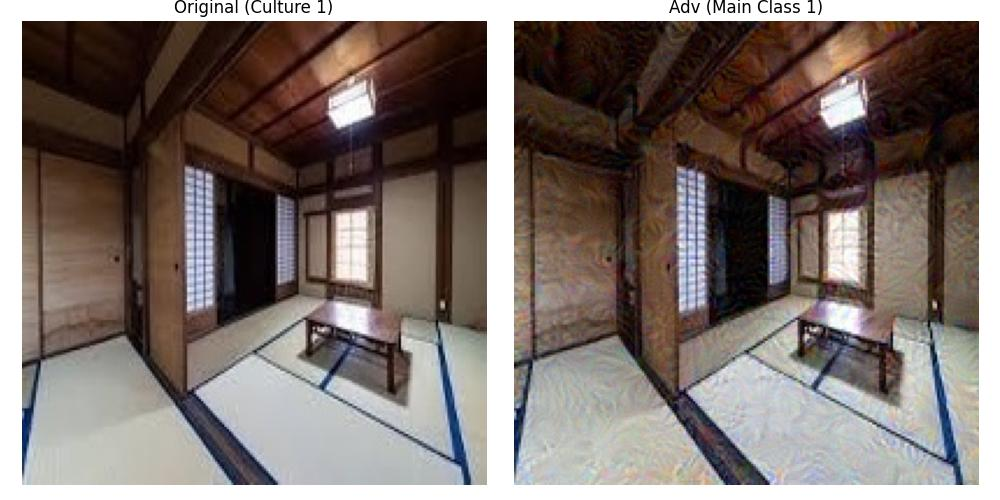
\includegraphics[width=\columnwidth]{adv_gen_figures/ADVmajCI_NOCLSDIV1_source_1.jpg}
\end{subfigure} \\
\begin{subfigure}[b]{0.6\columnwidth}
\centering
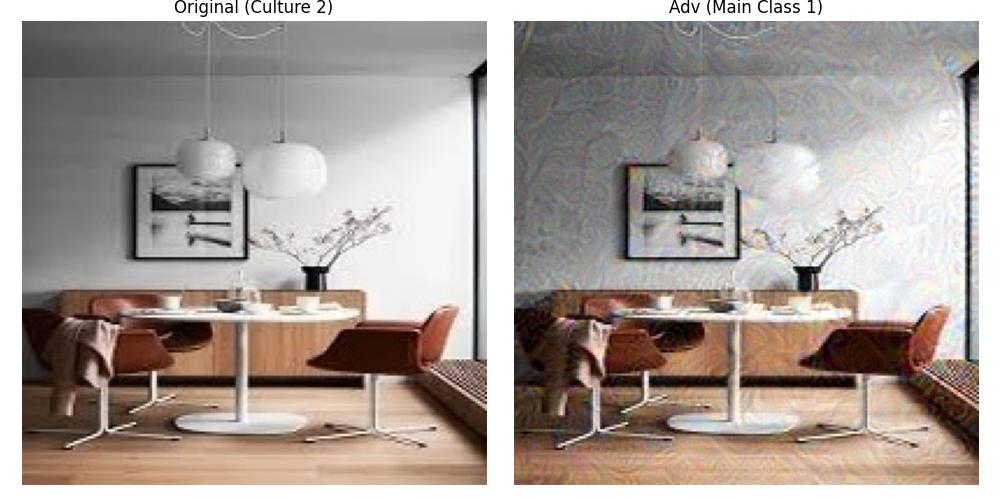
\includegraphics[width=\columnwidth]{adv_gen_figures/ADVmajCI_NOCLSDIV1_source_2.jpg}
\end{subfigure} 
\caption{Example of transformations applied on Ind. Jap. and Scan. dataset without carpets using PGD and NOCLSDIV with Ind. as majority culture.}
\label{fig::advCI_NOCLSDIV1}
\end{figure}

\begin{figure}[H]
\centering
\begin{subfigure}[b]{0.6\columnwidth}
\centering
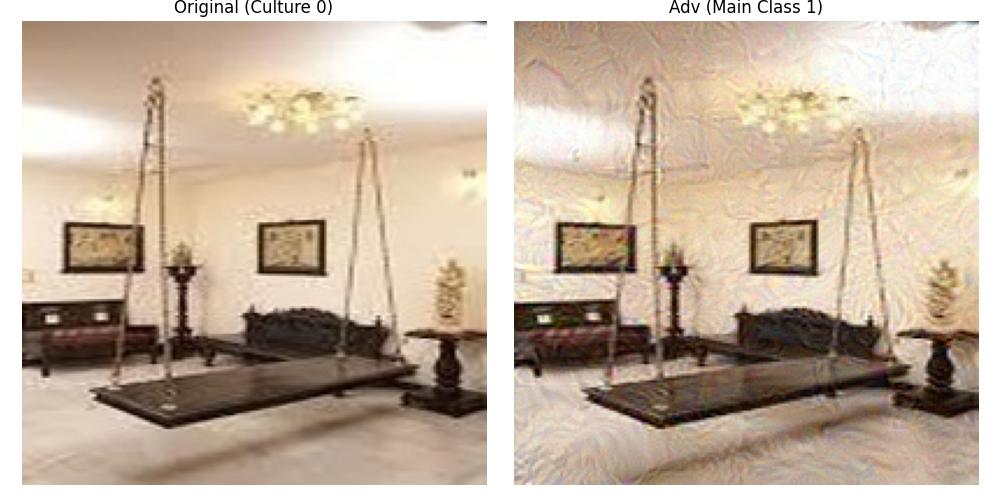
\includegraphics[width=\columnwidth]{adv_gen_figures/ADVmajCJ_NOCLSDIV1_source_0.jpg}
\end{subfigure} \\
\begin{subfigure}[b]{0.6\columnwidth}
\centering
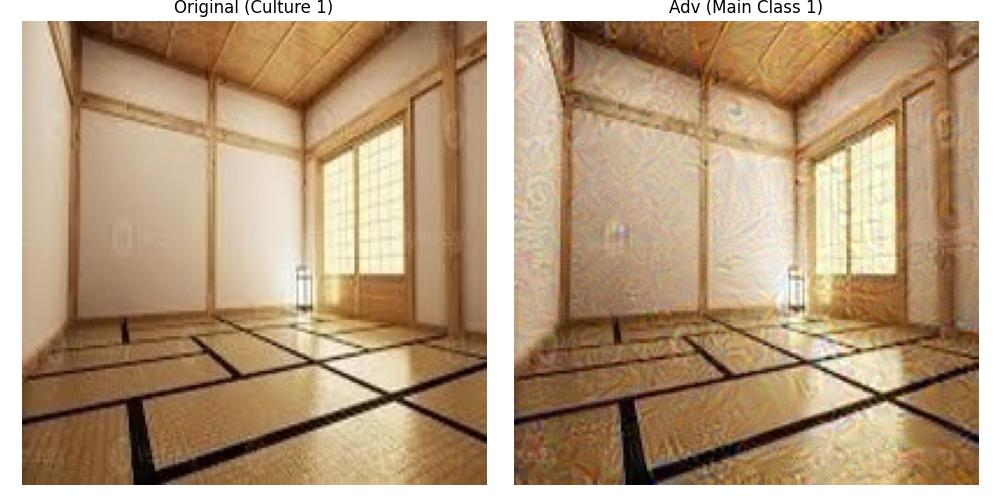
\includegraphics[width=\columnwidth]{adv_gen_figures/ADVmajCJ_NOCLSDIV1_source_1.jpg}
\end{subfigure} \\
\begin{subfigure}[b]{0.6\columnwidth}
\centering
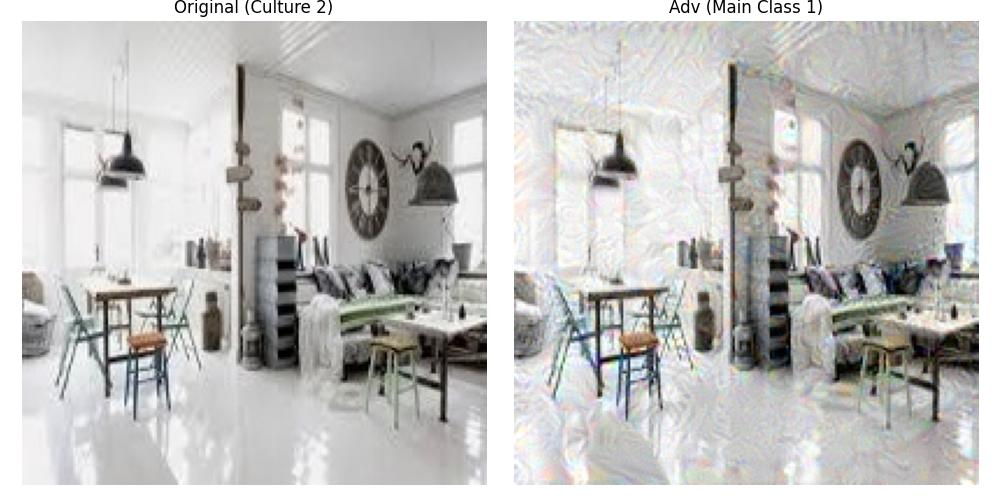
\includegraphics[width=\columnwidth]{adv_gen_figures/ADVmajCJ_NOCLSDIV1_source_2.jpg}
\end{subfigure} 
\caption{Example of transformations applied on Ind. Jap. and Scan. dataset without carpets using PGD and NOCLSDIV with Jap. as majority culture.}
\label{fig::advCJ_NOCLSDIV1}
\end{figure}

\begin{figure}[H]
\centering
\begin{subfigure}[b]{0.6\columnwidth}
\centering
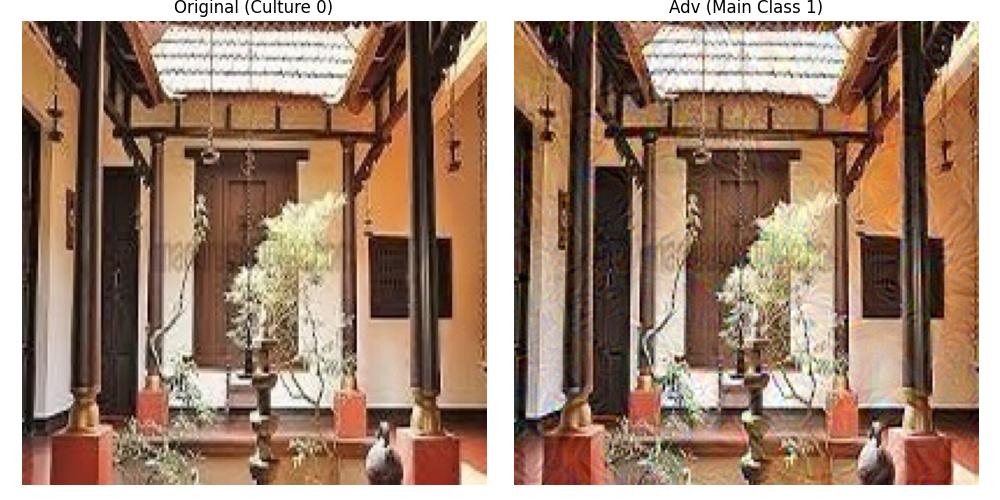
\includegraphics[width=\columnwidth]{adv_gen_figures/ADVmajCS_NOCLSDIV1_source_0.jpg}
\end{subfigure} \\
\begin{subfigure}[b]{0.6\columnwidth}
\centering
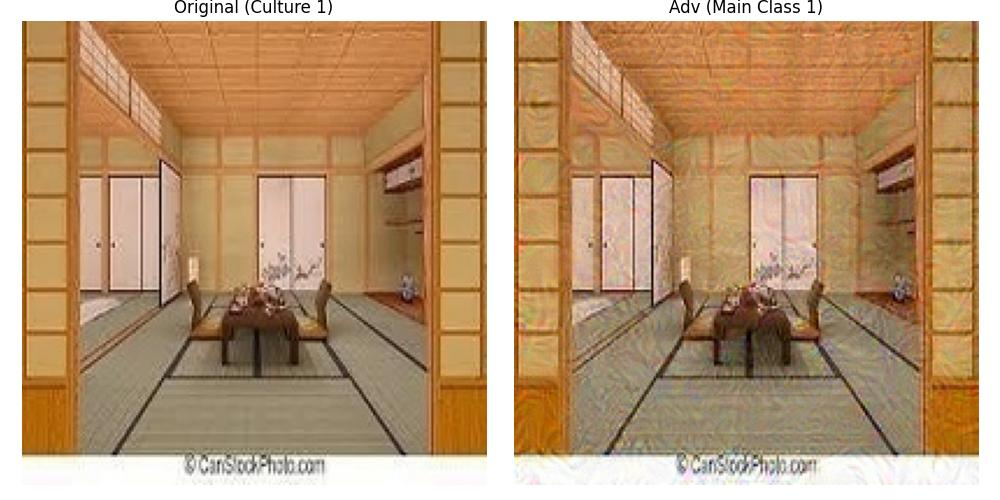
\includegraphics[width=\columnwidth]{adv_gen_figures/ADVmajCS_NOCLSDIV1_source_1.jpg}
\end{subfigure} \\
\begin{subfigure}[b]{0.6\columnwidth}
\centering
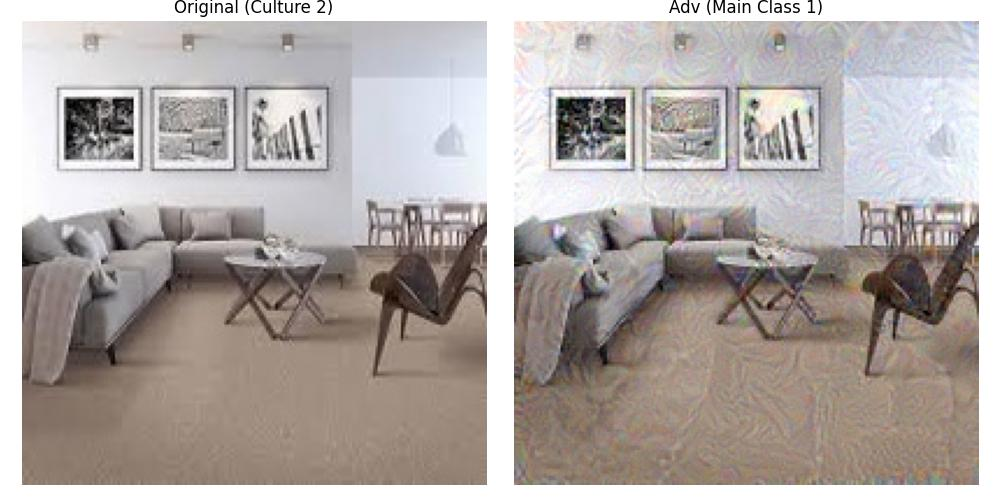
\includegraphics[width=\columnwidth]{adv_gen_figures/ADVmajCS_NOCLSDIV1_source_2.jpg}
\end{subfigure} 
\caption{Example of transformations applied on Ind. Jap. and Scan. dataset without carpets using PGD and NOCLSDIV with Scan. as majority culture.}
\label{fig::advCS_NOCLSDIV1}
\end{figure}

% RT
Tables~\ref{fig::advrtLC_CLSDIV0}, \ref{fig::advrtLC_CLSDIV1}, \ref{fig::advrtLC_NOCLSDIV0}, \ref{fig::advrtLC_NOCLSDIV1}, \ref{fig::advrtLF_CLSDIV0}, \ref{fig::advrtLF_CLSDIV1}, \ref{fig::advrtLF_NOCLSDIV0}, \ref{fig::advrtLF_NOCLSDIV1},
\ref{fig::advrtLT_CLSDIV0}, \ref{fig::advrtLT_CLSDIV1}, \ref{fig::advrtLT_NOCLSDIV0}, \ref{fig::advrtLT_NOCLSDIV1} show examples of transformations applied on Chin., Fren. and Turk. images from LAMP dataset with lamps turned off using PGD, RT and CLSDIV or NOCLSDIV with Chin., Fren. and Turk as majority cultures.
%CLSDIV 0
\begin{figure}[H]
\centering
\begin{subfigure}[b]{0.6\columnwidth}
\centering
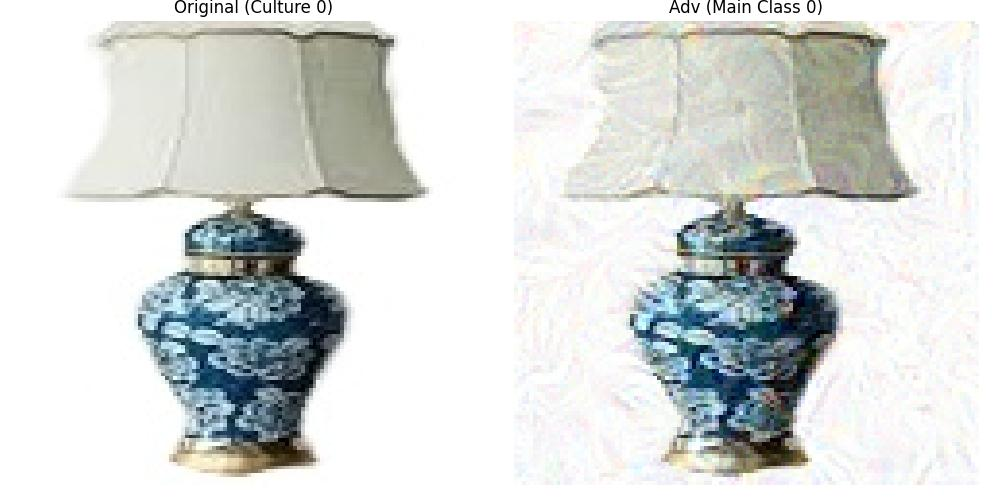
\includegraphics[width=\columnwidth]{adv_gen_figures/adv_rt_LC_CLSDIV0_source0.jpg}
\end{subfigure} \\
\begin{subfigure}[b]{0.6\columnwidth}
\centering
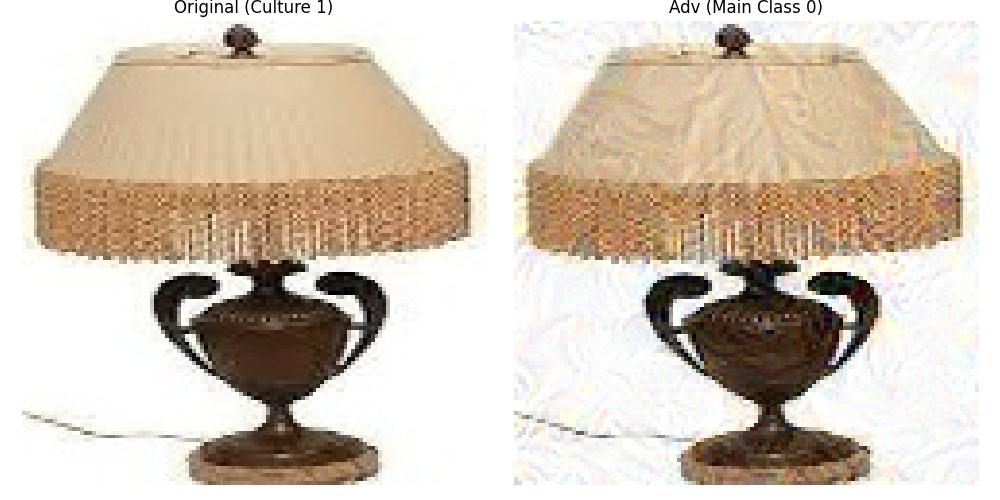
\includegraphics[width=\columnwidth]{adv_gen_figures/adv_rt_LC_CLSDIV0_source1.jpg}
\end{subfigure} \\
\begin{subfigure}[b]{0.6\columnwidth}
\centering
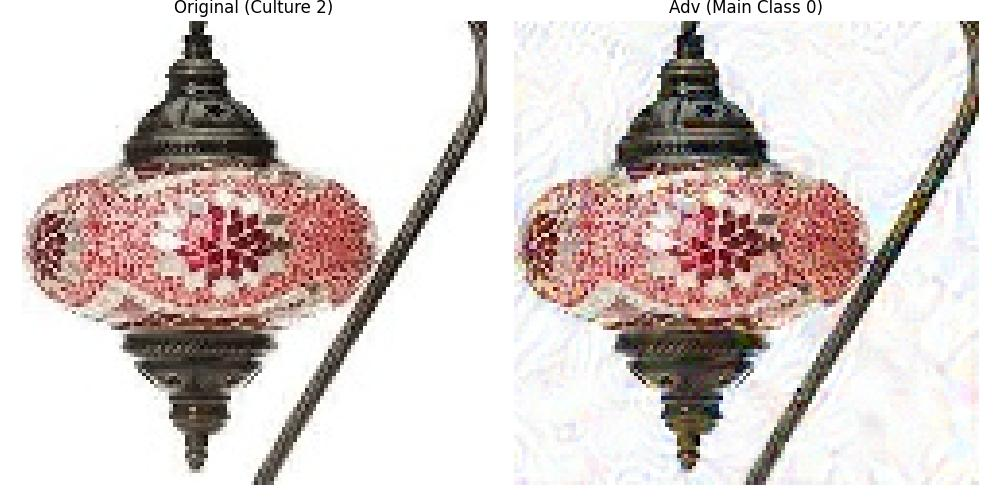
\includegraphics[width=\columnwidth]{adv_gen_figures/adv_rt_LC_CLSDIV0_source2.jpg}
\end{subfigure} 
\caption{Example of transformations applied on Chin., Fren. and Turk. images from LAMP dataset with lamps turned off using PGD, RT and CLSDIV with Chin. as majority culture.}
\label{fig::advrtLC_CLSDIV0}
\end{figure}

\begin{figure}[H]
\centering
\begin{subfigure}[b]{0.6\columnwidth}
\centering
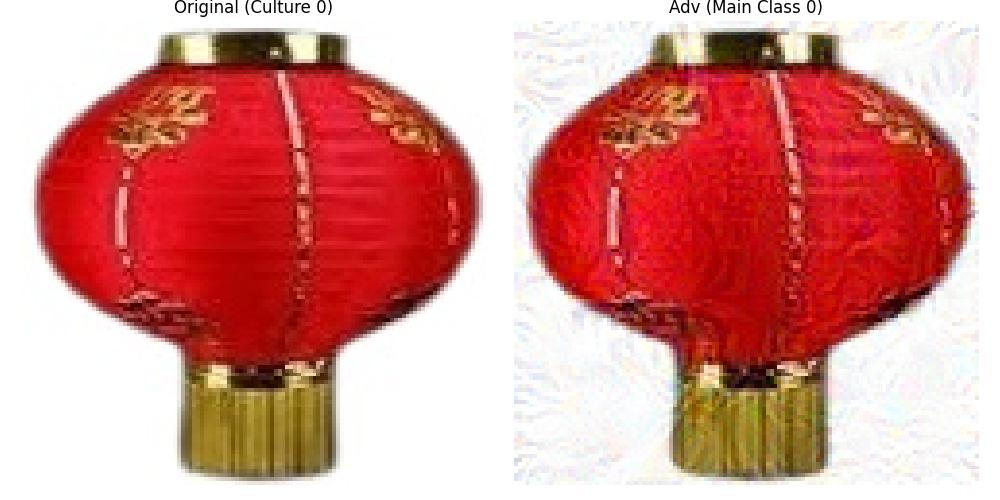
\includegraphics[width=\columnwidth]{adv_gen_figures/adv_rt_LF_CLSDIV0_source0.jpg}

\end{subfigure} \\
\begin{subfigure}[b]{0.6\columnwidth}
\centering
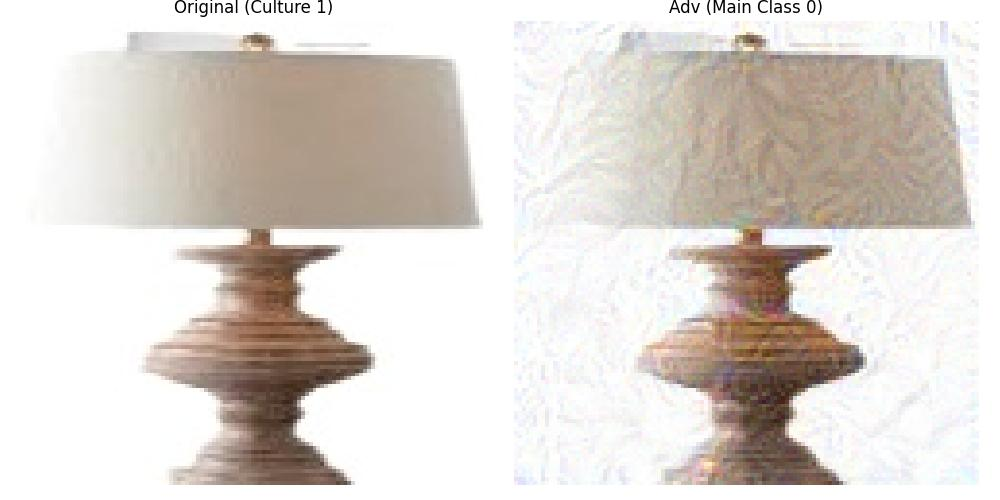
\includegraphics[width=\columnwidth]{adv_gen_figures/adv_rt_LF_CLSDIV0_source1.jpg}
\end{subfigure} \\
\begin{subfigure}[b]{0.6\columnwidth}
\centering
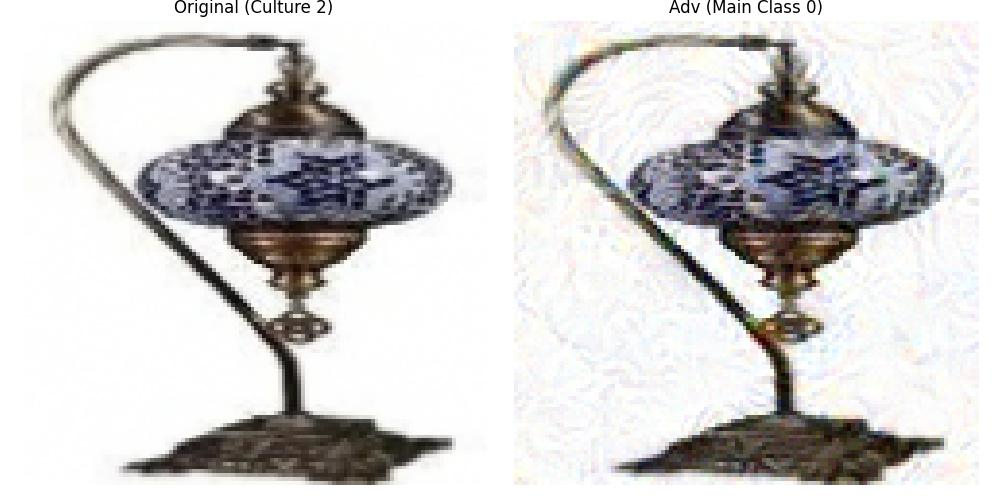
\includegraphics[width=\columnwidth]{adv_gen_figures/adv_rt_LF_CLSDIV0_source2.jpg}
\end{subfigure} 
\caption{Example of transformations applied on Chin., Fren. and Turk. images from LAMP dataset with lamps turned off using PGD, RT and CLSDIV with Fren. as majority culture.}
\label{fig::advrtLF_CLSDIV0}
\end{figure}

\begin{figure}[H]
\centering
\begin{subfigure}[b]{0.6\columnwidth}
\centering
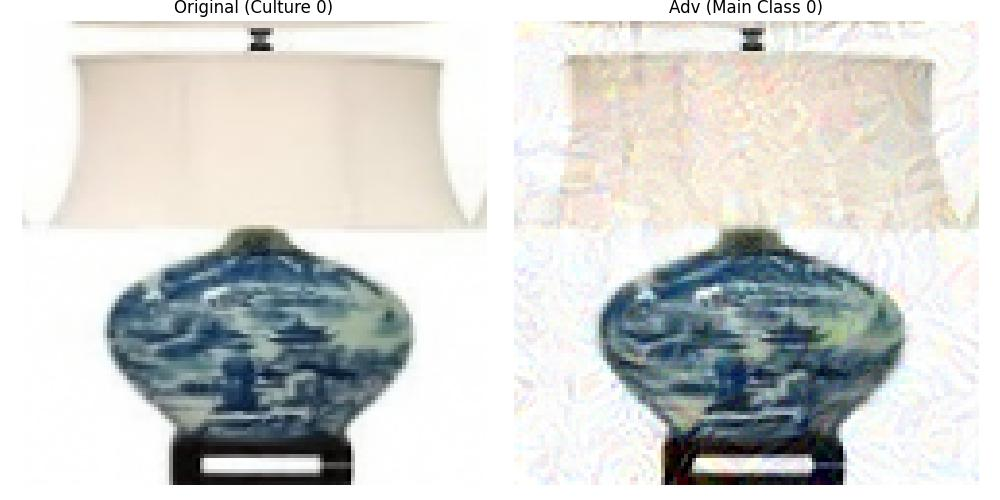
\includegraphics[width=\columnwidth]{adv_gen_figures/adv_rt_LT_CLSDIV0_source0.jpg}
\end{subfigure} \\
\begin{subfigure}[b]{0.6\columnwidth}
\centering
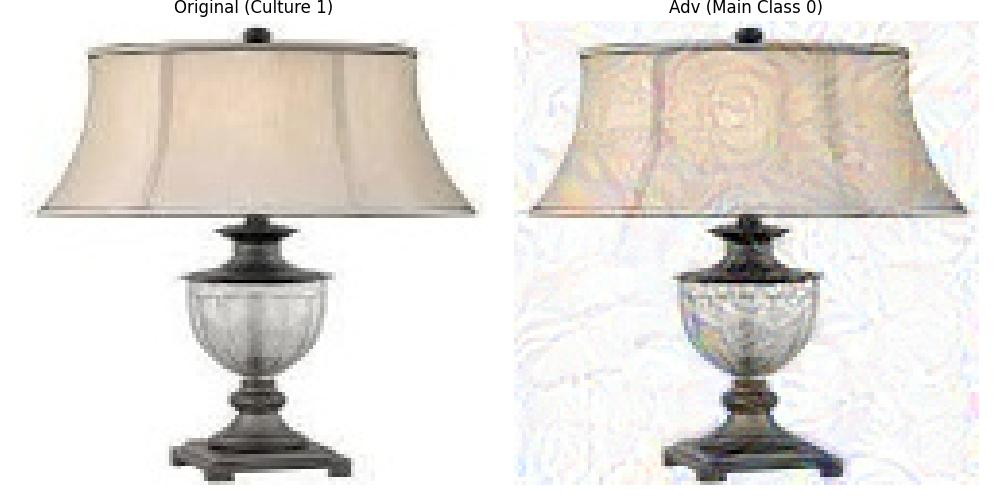
\includegraphics[width=\columnwidth]{adv_gen_figures/adv_rt_LT_CLSDIV0_source1.jpg}
\end{subfigure} \\
\begin{subfigure}[b]{0.6\columnwidth}
\centering
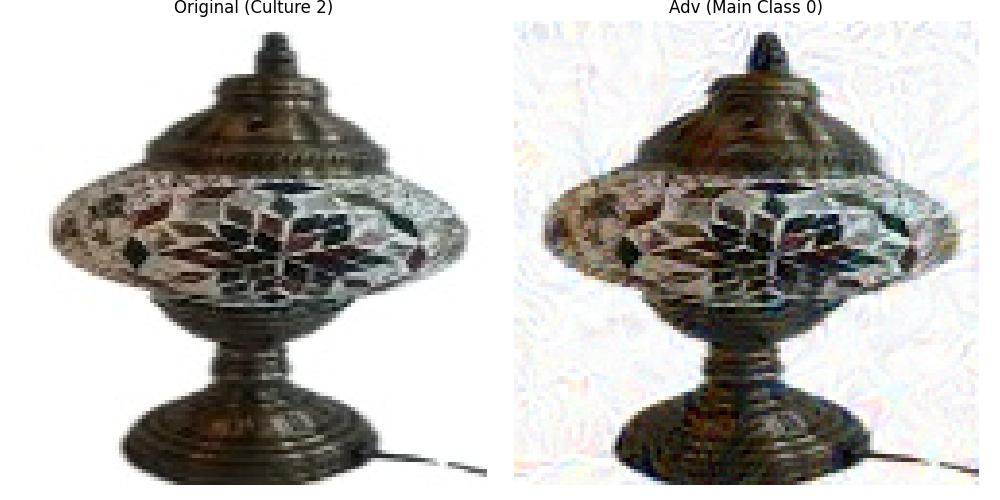
\includegraphics[width=\columnwidth]{adv_gen_figures/adv_rt_LT_CLSDIV0_source2.jpg}
\end{subfigure} 
\caption{Example of transformations applied on Chin., Fren. and Turk. images from LAMP dataset with lamps turned off using PGD, RT and CLSDIV with Turk. as majority culture.}
\label{fig::advrtLT_CLSDIV0}
\end{figure}

%CLSDIV 1
\begin{figure}[H]
\centering
\begin{subfigure}[b]{0.6\columnwidth}
\centering
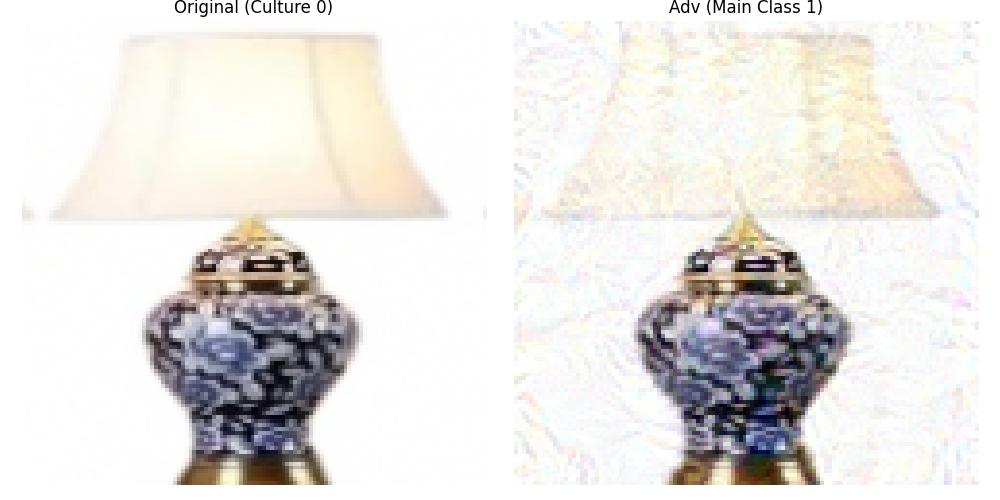
\includegraphics[width=\columnwidth]{adv_gen_figures/adv_rt_LC_CLSDIV1_source0.jpg}
\end{subfigure} \\
\begin{subfigure}[b]{0.6\columnwidth}
\centering
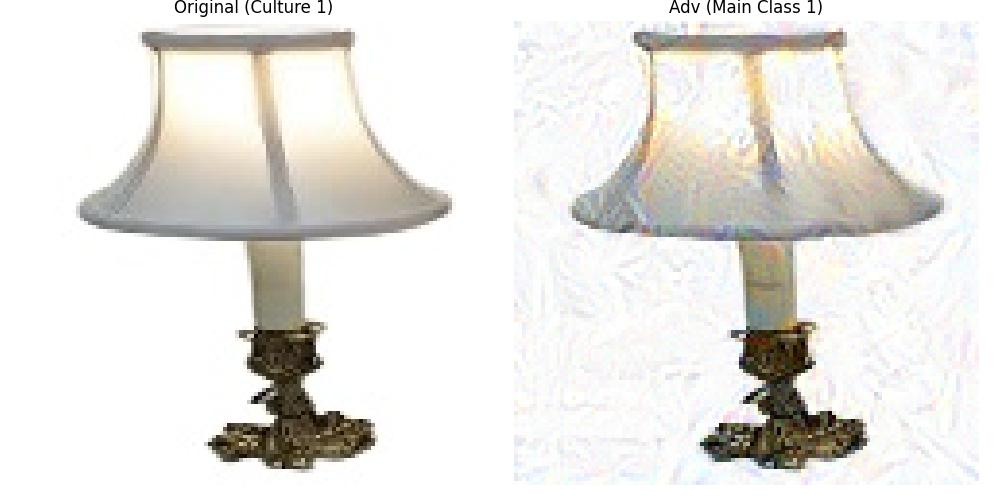
\includegraphics[width=\columnwidth]{adv_gen_figures/adv_rt_LC_CLSDIV1_source1.jpg}
\end{subfigure} \\
\begin{subfigure}[b]{0.6\columnwidth}
\centering
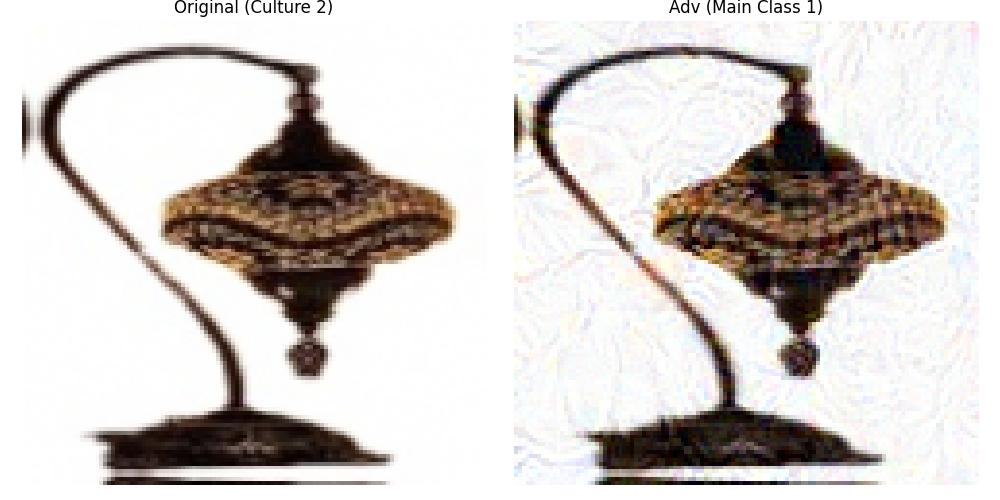
\includegraphics[width=\columnwidth]{adv_gen_figures/adv_rt_LC_CLSDIV1_source2.jpg}
\end{subfigure} 
\caption{Example of transformations applied on Chin., Fren. and Turk. images from LAMP dataset with lamps turned on using PGD, RT and CLSDIV with Chin. as majority culture.}
\label{fig::advrtLC_CLSDIV1}
\end{figure}

\begin{figure}[H]
\centering
\begin{subfigure}[b]{0.6\columnwidth}
\centering
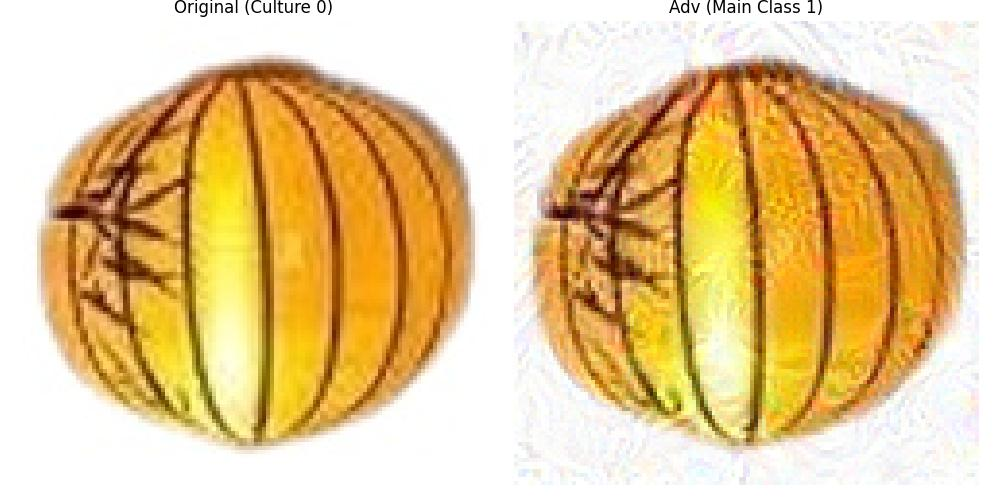
\includegraphics[width=\columnwidth]{adv_gen_figures/adv_rt_LF_CLSDIV1_source0.jpg}
\end{subfigure} \\
\begin{subfigure}[b]{0.6\columnwidth}
\centering
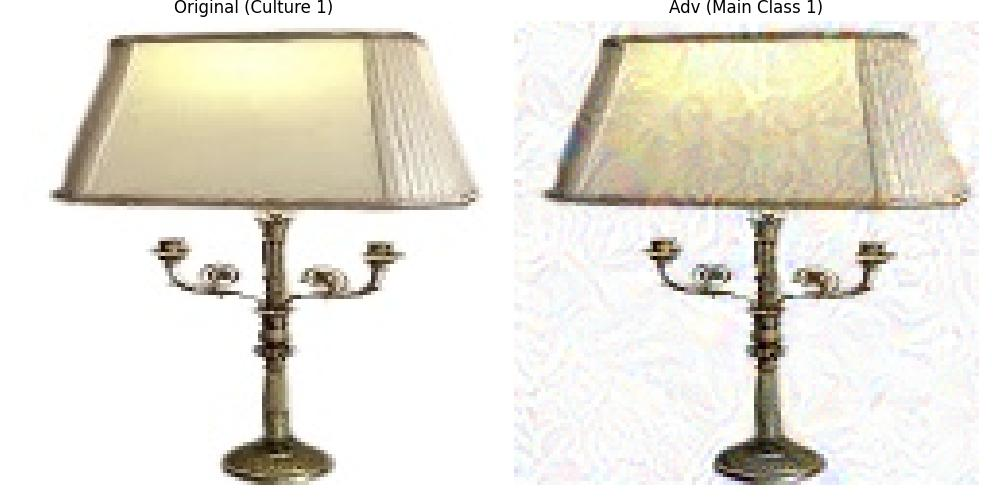
\includegraphics[width=\columnwidth]{adv_gen_figures/adv_rt_LF_CLSDIV1_source1.jpg}
\end{subfigure} \\
\begin{subfigure}[b]{0.6\columnwidth}
\centering
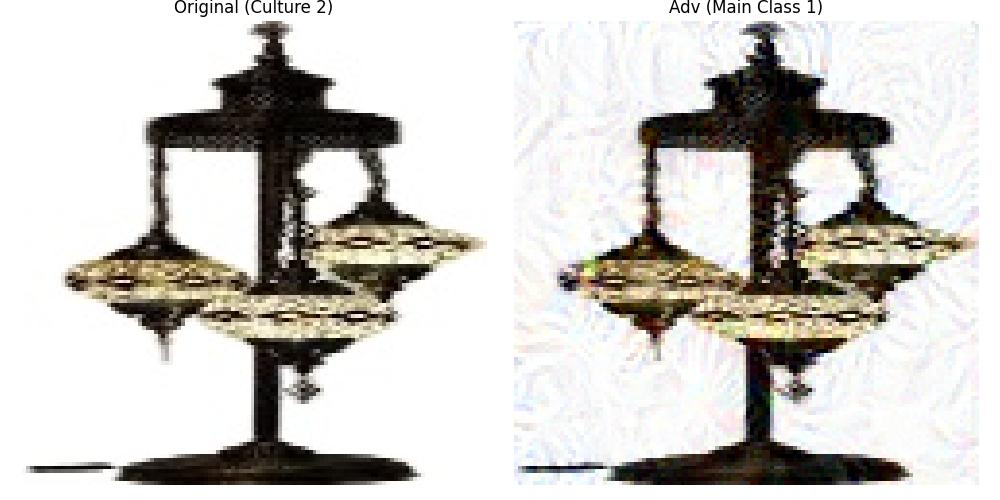
\includegraphics[width=\columnwidth]{adv_gen_figures/adv_rt_LF_CLSDIV1_source2.jpg}
\end{subfigure} 
\caption{Example of transformations applied on Chin., Fren. and Turk. images from LAMP dataset with lamps turned on using PGD, RT and CLSDIV with Fren. as majority culture.}
\label{fig::advrtLF_CLSDIV1}
\end{figure}

\begin{figure}[H]
\centering
\begin{subfigure}[b]{0.6\columnwidth}
\centering
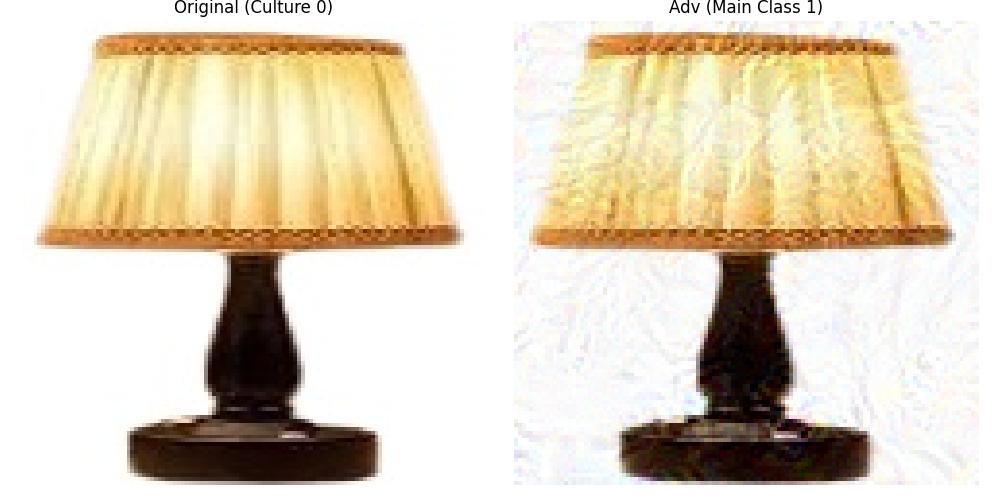
\includegraphics[width=\columnwidth]{adv_gen_figures/adv_rt_LT_CLSDIV1_source0.jpg}
\end{subfigure} \\
\begin{subfigure}[b]{0.6\columnwidth}
\centering
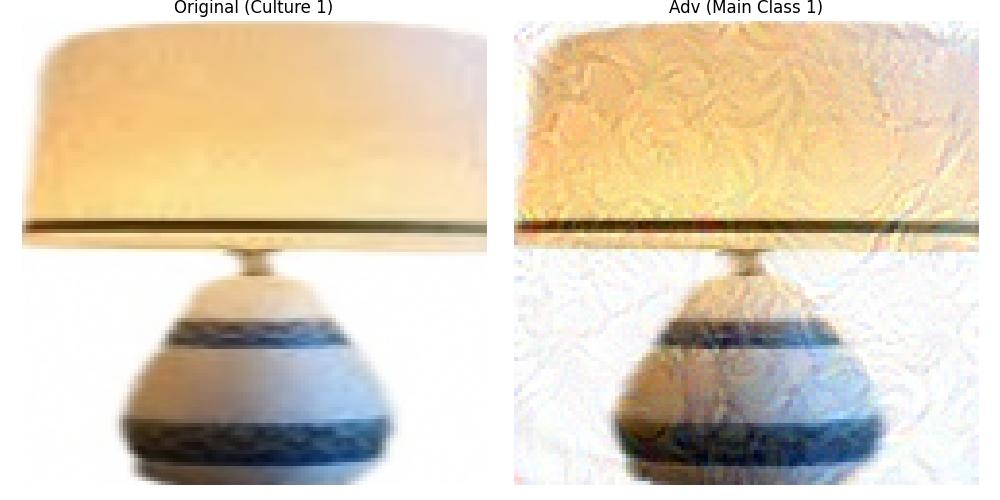
\includegraphics[width=\columnwidth]{adv_gen_figures/adv_rt_LT_CLSDIV1_source1.jpg}
\end{subfigure} \\
\begin{subfigure}[b]{0.6\columnwidth}
\centering
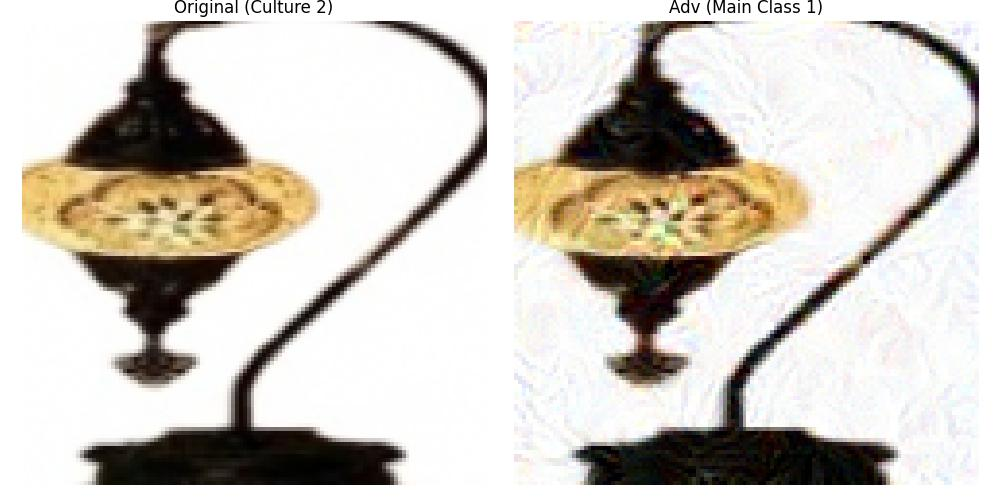
\includegraphics[width=\columnwidth]{adv_gen_figures/adv_rt_LT_CLSDIV1_source2.jpg}
\end{subfigure} 
\caption{Example of transformations applied on Chin., Fren. and Turk. images from LAMP dataset with lamps turned on using PGD, RT and CLSDIV with Turk. as majority culture.}
\label{fig::advrtLT_CLSDIV1}
\end{figure}

% NOCLSDIV 0
\begin{figure}[H]
\centering
\begin{subfigure}[b]{0.6\columnwidth}
\centering
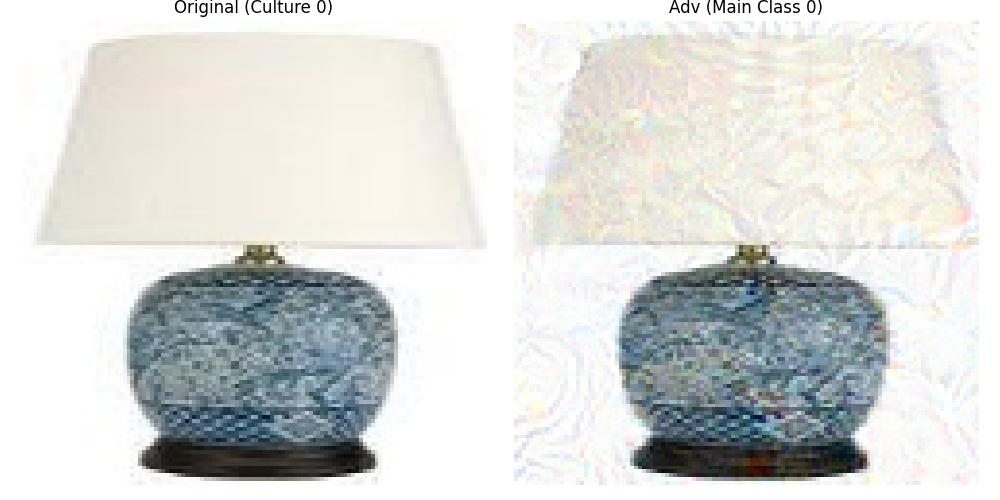
\includegraphics[width=\columnwidth]{adv_gen_figures/adv_rt_LC_NOCLSDIV0_source0.jpg}
\end{subfigure} \\
\begin{subfigure}[b]{0.6\columnwidth}
\centering
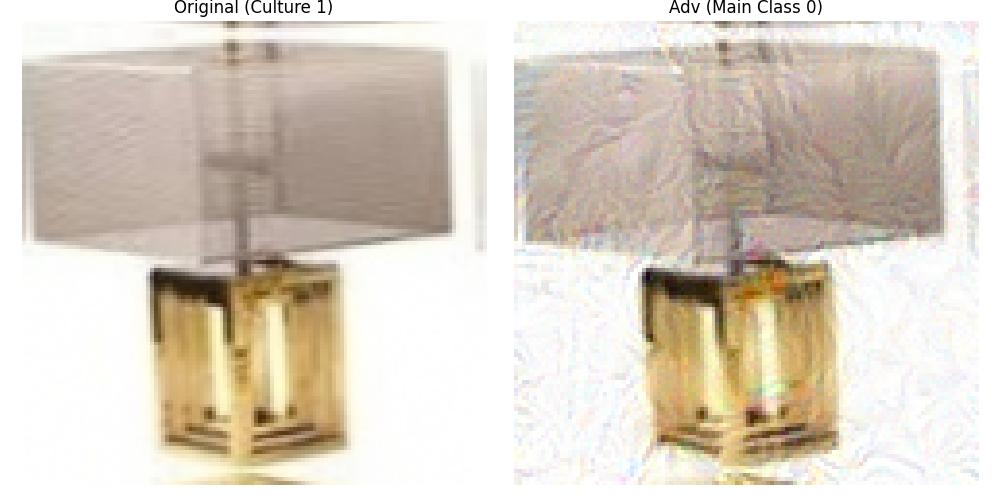
\includegraphics[width=\columnwidth]{adv_gen_figures/adv_rt_LC_NOCLSDIV0_source1.jpg}
\end{subfigure} \\
\begin{subfigure}[b]{0.6\columnwidth}
\centering
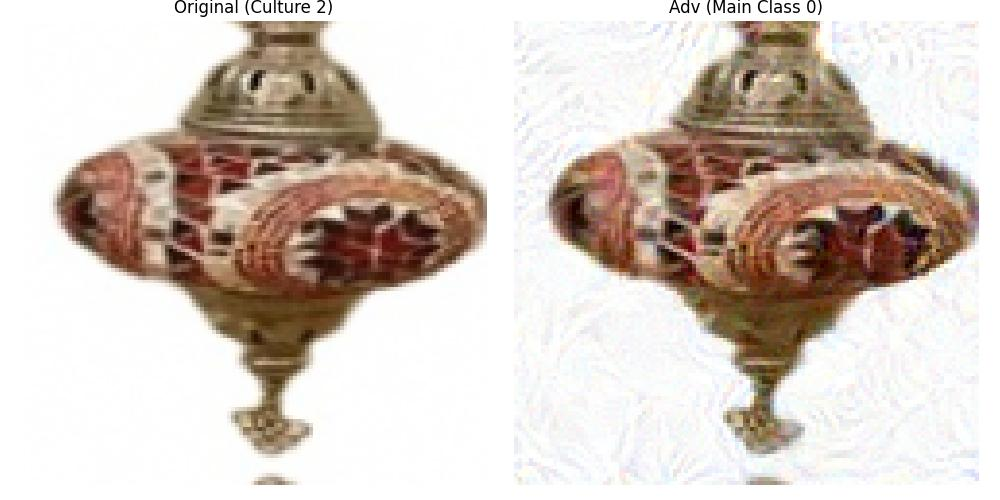
\includegraphics[width=\columnwidth]{adv_gen_figures/adv_rt_LC_NOCLSDIV0_source2.jpg}
\end{subfigure} 
\caption{Example of transformations applied on Chin., Fren. and Turk. images from LAMP dataset with lamps turned off using PGD, RT and NOCLSDIV with Chin. as majority culture.}
\label{fig::advrtLC_NOCLSDIV0}
\end{figure}

\begin{figure}[H]
\centering
\begin{subfigure}[b]{0.6\columnwidth}
\centering
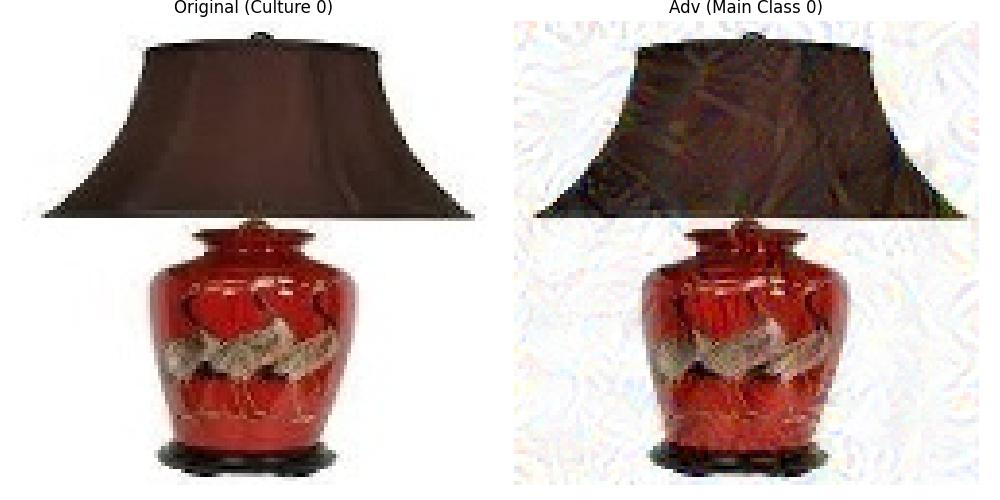
\includegraphics[width=\columnwidth]{adv_gen_figures/adv_rt_LF_NOCLSDIV0_source0.jpg}
\end{subfigure} \\
\begin{subfigure}[b]{0.6\columnwidth}
\centering
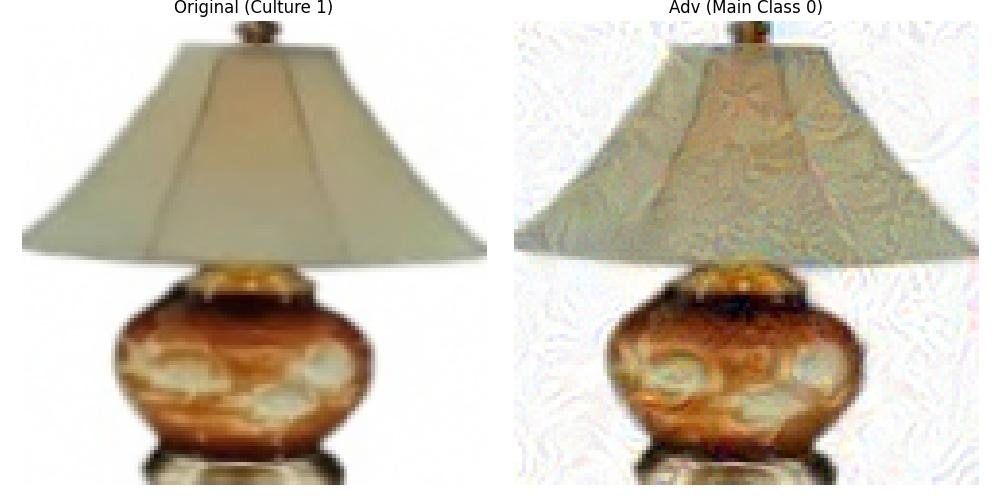
\includegraphics[width=\columnwidth]{adv_gen_figures/adv_rt_LF_NOCLSDIV0_source1.jpg}
\end{subfigure} \\
\begin{subfigure}[b]{0.6\columnwidth}
\centering
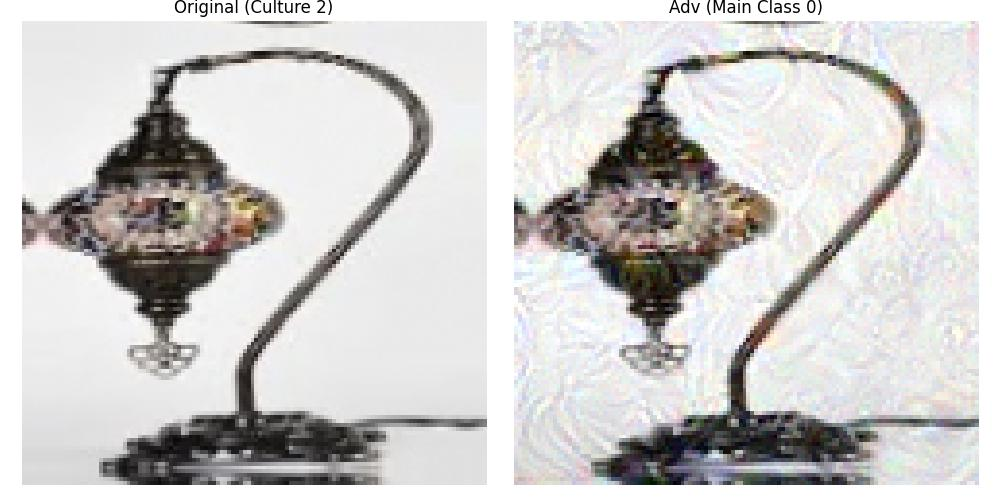
\includegraphics[width=\columnwidth]{adv_gen_figures/adv_rt_LF_NOCLSDIV0_source2.jpg}
\end{subfigure} 
\caption{Example of transformations applied on Chin., Fren. and Turk. images from LAMP dataset with lamps turned off using PGD, RT and NOCLSDIV with Fren. as majority culture.}
\label{fig::advrtLF_NOCLSDIV0}
\end{figure}

\begin{figure}[H]
\centering
\begin{subfigure}[b]{0.6\columnwidth}
\centering
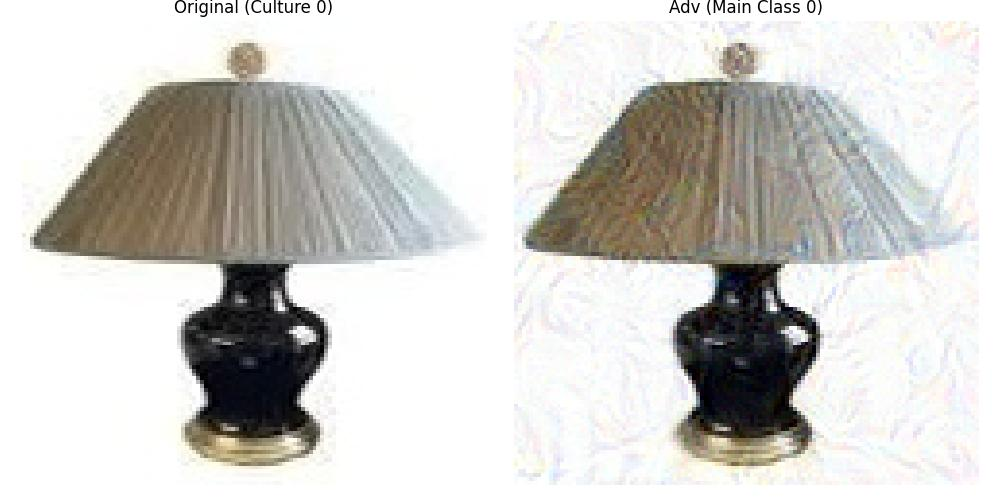
\includegraphics[width=\columnwidth]{adv_gen_figures/adv_rt_LT_NOCLSDIV0_source0.jpg}
\end{subfigure} \\
\begin{subfigure}[b]{0.6\columnwidth}
\centering
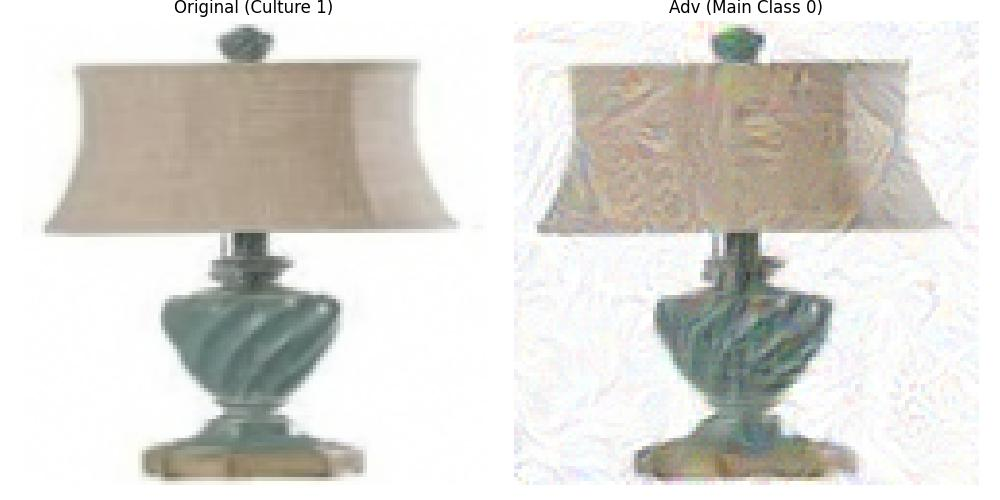
\includegraphics[width=\columnwidth]{adv_gen_figures/adv_rt_LT_NOCLSDIV0_source1.jpg}
\end{subfigure} \\
\begin{subfigure}[b]{0.6\columnwidth}
\centering
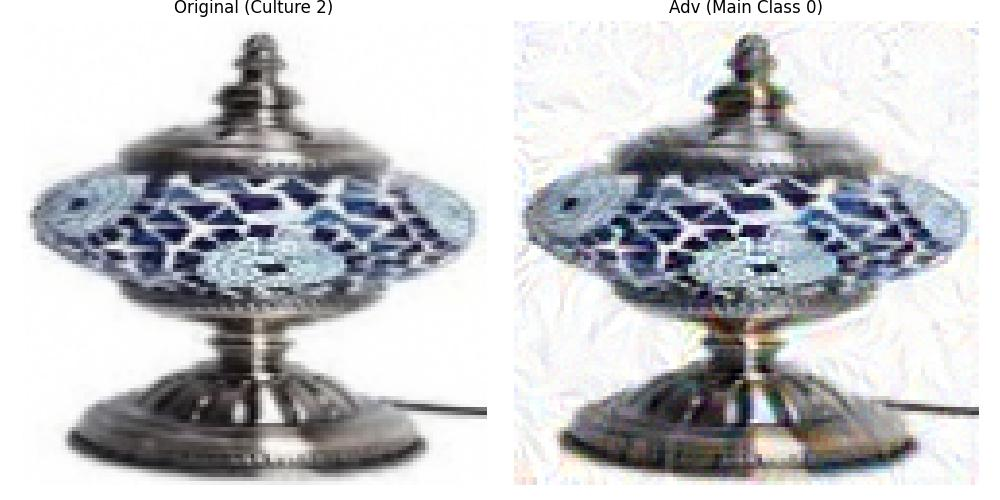
\includegraphics[width=\columnwidth]{adv_gen_figures/adv_rt_LT_NOCLSDIV0_source2.jpg}
\end{subfigure} 
\caption{Example of transformations applied on Chin., Fren. and Turk. images from LAMP dataset with lamps turned off using PGD, RT and NOCLSDIV with Turk. as majority culture.}
\label{fig::advrtLT_NOCLSDIV0}
\end{figure}

% NOCLSDIV 1
\begin{figure}[H]
\centering
\begin{subfigure}[b]{0.6\columnwidth}
\centering
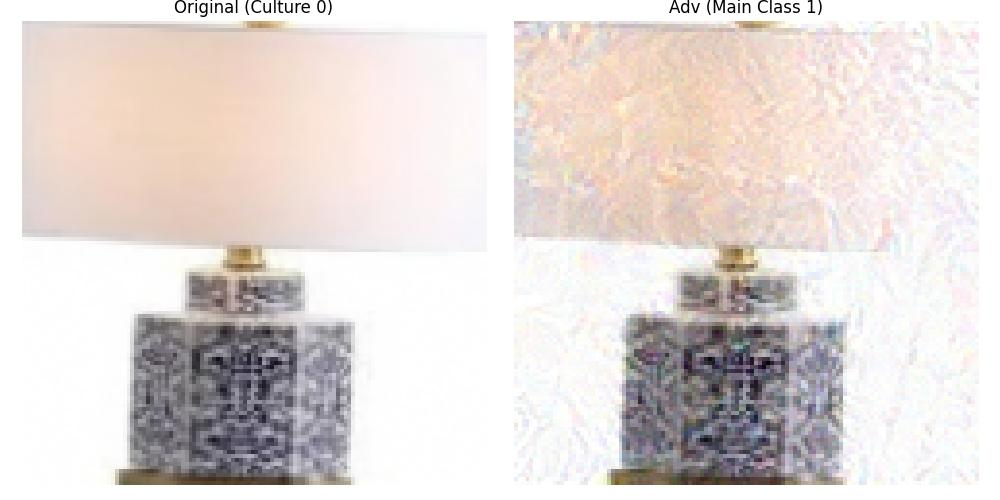
\includegraphics[width=\columnwidth]{adv_gen_figures/adv_rt_LC_NOCLSDIV1_source0.jpg}
\end{subfigure} \\
\begin{subfigure}[b]{0.6\columnwidth}
\centering
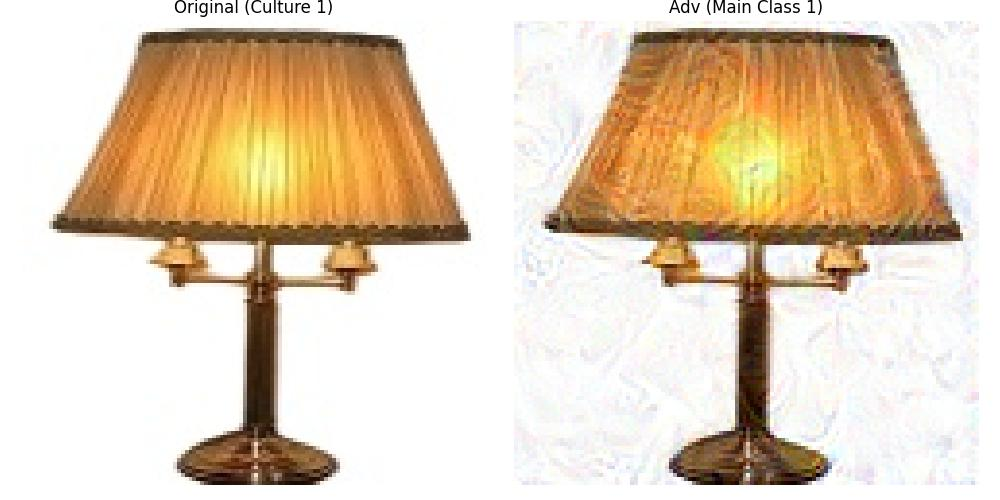
\includegraphics[width=\columnwidth]{adv_gen_figures/adv_rt_LC_NOCLSDIV1_source1.jpg}
\end{subfigure} \\
\begin{subfigure}[b]{0.6\columnwidth}
\centering
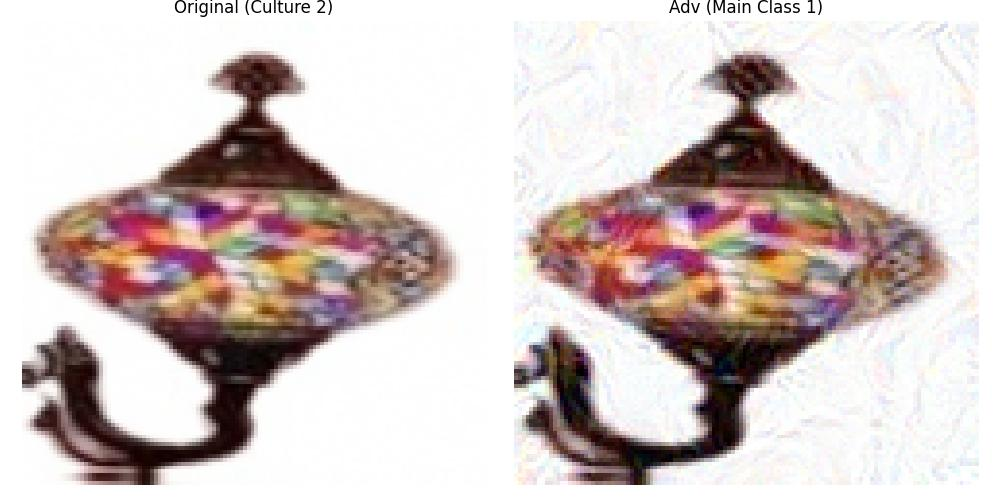
\includegraphics[width=\columnwidth]{adv_gen_figures/adv_rt_LC_NOCLSDIV1_source2.jpg}
\end{subfigure} 
\caption{Example of transformations applied on Chin., Fren. and Turk. images from LAMP dataset with lamps turned on using PGD, RT and NOCLSDIV with Chin. as majority culture.}
\label{fig::advrtLC_NOCLSDIV1}
\end{figure}

\begin{figure}[H]
\centering
\begin{subfigure}[b]{0.6\columnwidth}
\centering
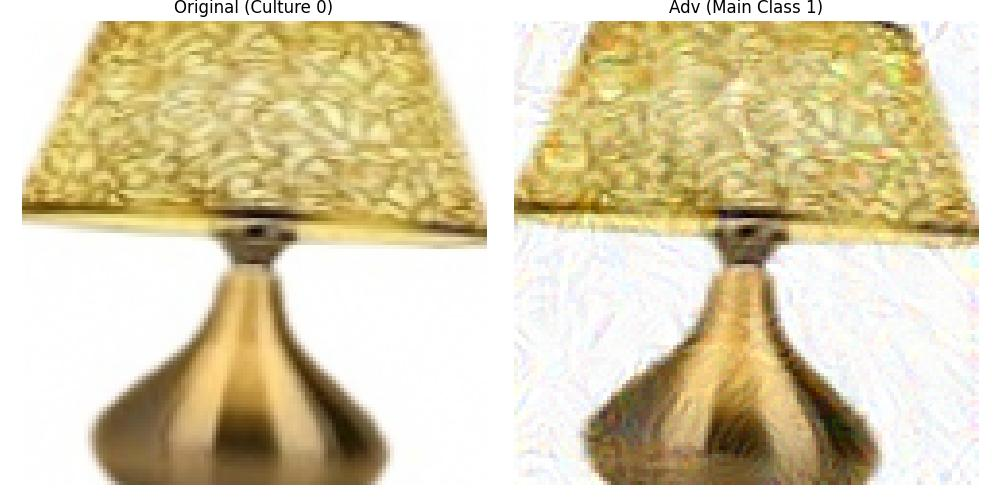
\includegraphics[width=\columnwidth]{adv_gen_figures/adv_rt_LF_NOCLSDIV1_source0.jpg}
\end{subfigure} \\
\begin{subfigure}[b]{0.6\columnwidth}
\centering
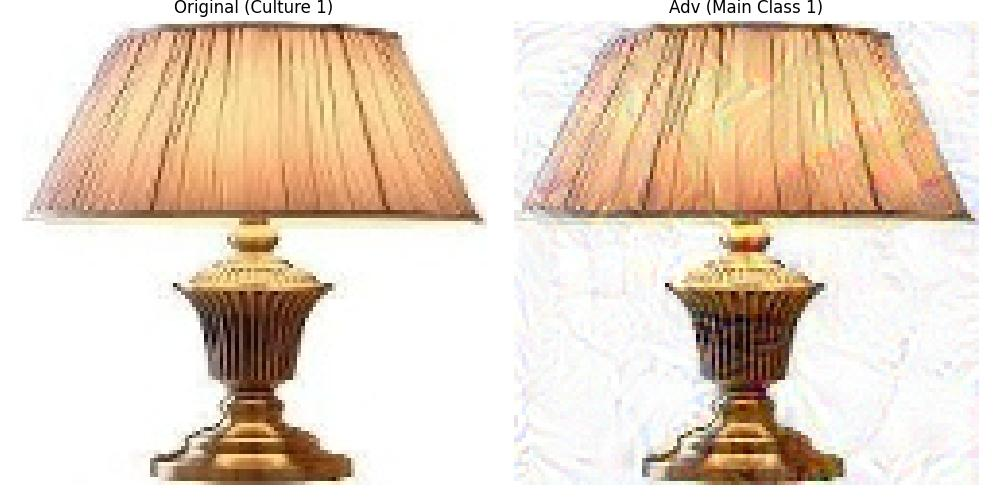
\includegraphics[width=\columnwidth]{adv_gen_figures/adv_rt_LF_NOCLSDIV1_source1.jpg}
\end{subfigure} \\
\begin{subfigure}[b]{0.6\columnwidth}
\centering
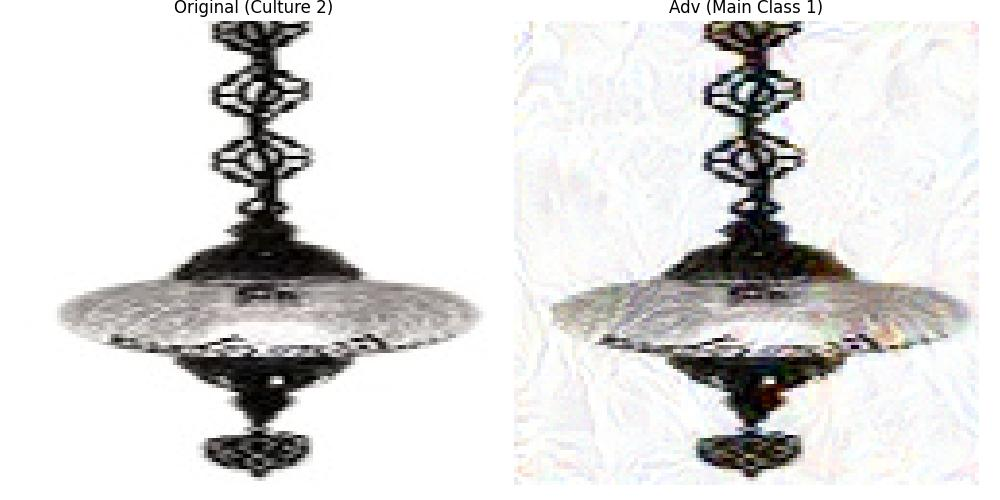
\includegraphics[width=\columnwidth]{adv_gen_figures/adv_rt_LF_NOCLSDIV1_source2.jpg}
\end{subfigure} 
\caption{Example of transformations applied on Chin., Fren. and Turk. images from LAMP dataset with lamps turned on using PGD, RT and NOCLSDIV with Fren. as majority culture.}
\label{fig::advrtLF_NOCLSDIV1}
\end{figure}

\begin{figure}[H]
\centering
\begin{subfigure}[b]{0.6\columnwidth}
\centering
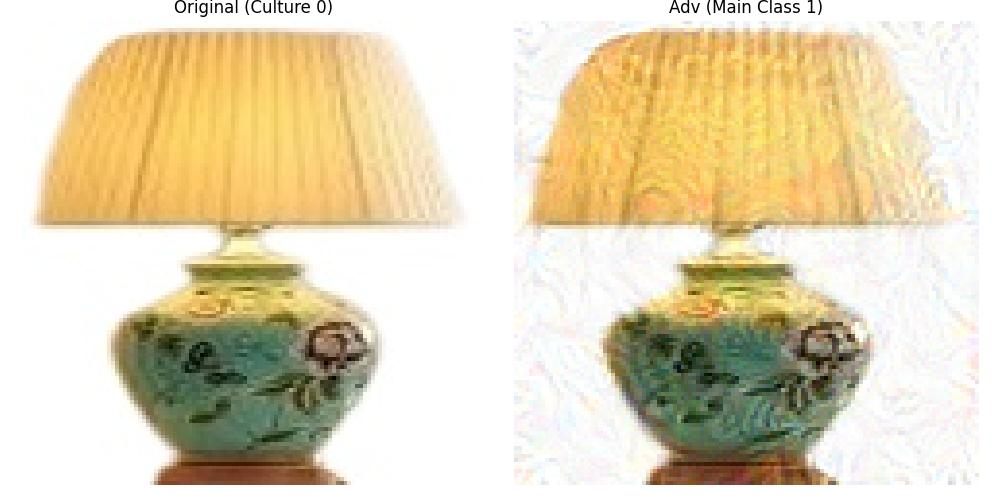
\includegraphics[width=\columnwidth]{adv_gen_figures/adv_rt_LT_NOCLSDIV1_source0.jpg}
\end{subfigure} \\
\begin{subfigure}[b]{0.6\columnwidth}
\centering
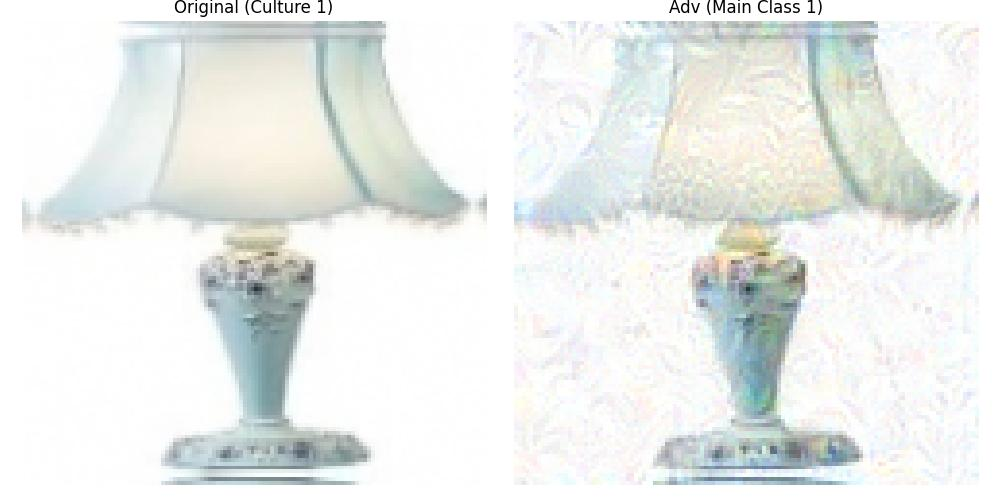
\includegraphics[width=\columnwidth]{adv_gen_figures/adv_rt_LT_NOCLSDIV1_source1.jpg}
\end{subfigure} \\
\begin{subfigure}[b]{0.6\columnwidth}
\centering
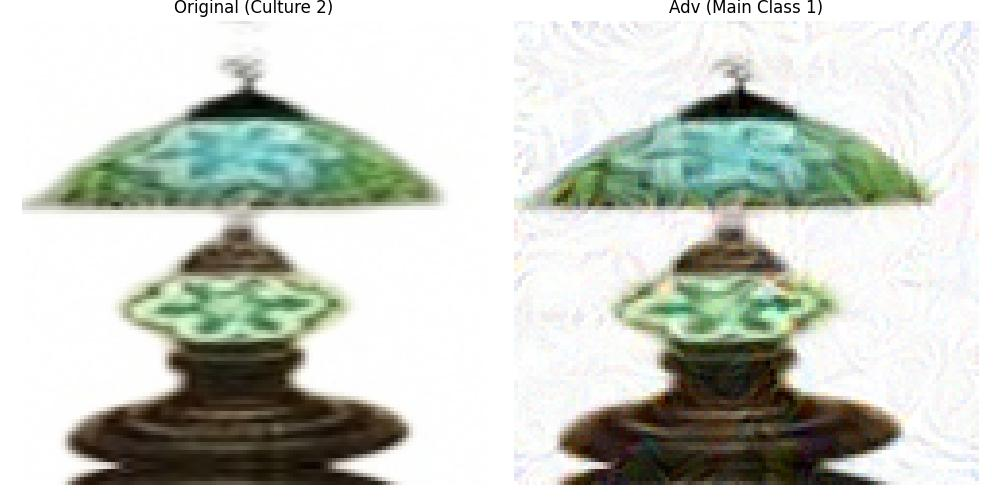
\includegraphics[width=\columnwidth]{adv_gen_figures/adv_rt_LT_NOCLSDIV1_source2.jpg}
\end{subfigure} 
\caption{Example of transformations applied on Chin., Fren. and Turk. images from LAMP dataset with lamps turned on using PGD, RT and NOCLSDIV with Turk. as majority culture.}
\label{fig::advrtLT_NOCLSDIV1}
\end{figure}

% CARPET
Tables~\ref{fig::advrtCI_CLSDIV0}, \ref{fig::advrtCI_CLSDIV1}, \ref{fig::advrtCI_NOCLSDIV0}, \ref{fig::advrtCI_NOCLSDIV1}, \ref{fig::advrtCJ_CLSDIV0}, \ref{fig::advrtCJ_CLSDIV1}, \ref{fig::advrtCJ_NOCLSDIV0}, \ref{fig::advrtCJ_NOCLSDIV1},
\ref{fig::advrtCS_CLSDIV0}, \ref{fig::advrtCS_CLSDIV1}, \ref{fig::advrtCS_NOCLSDIV0}, \ref{fig::advrtCS_NOCLSDIV1} show examples of transformations applied on Ind., Jap., and Scan. images from CARPET dataset with lamps turned off using PGD, RT and CLSDIV or NOCLSDIV with Ind., Jap., and Scan. as majority cultures.
\begin{figure}[H]
\centering
\begin{subfigure}[b]{0.6\columnwidth}
\centering
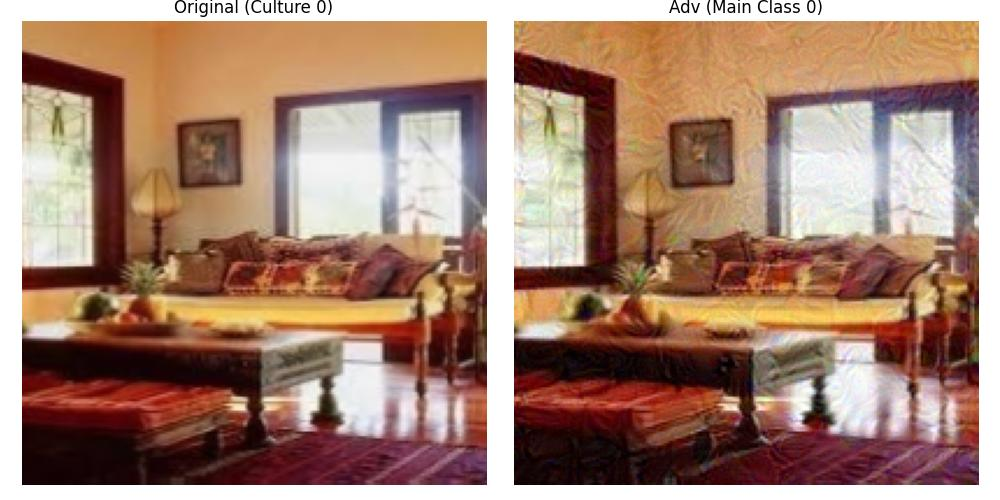
\includegraphics[width=\columnwidth]{adv_gen_figures/adv_rt_CI_CLSDIV0_source0.jpg}
\end{subfigure} \\
\begin{subfigure}[b]{0.6\columnwidth}
\centering
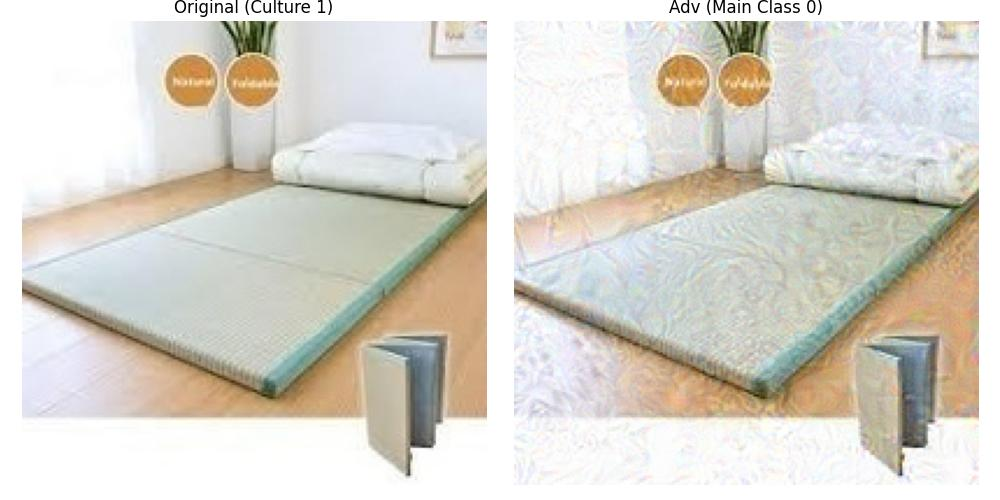
\includegraphics[width=\columnwidth]{adv_gen_figures/adv_rt_CI_CLSDIV0_source1.jpg}
\end{subfigure} \\
\begin{subfigure}[b]{0.6\columnwidth}
\centering
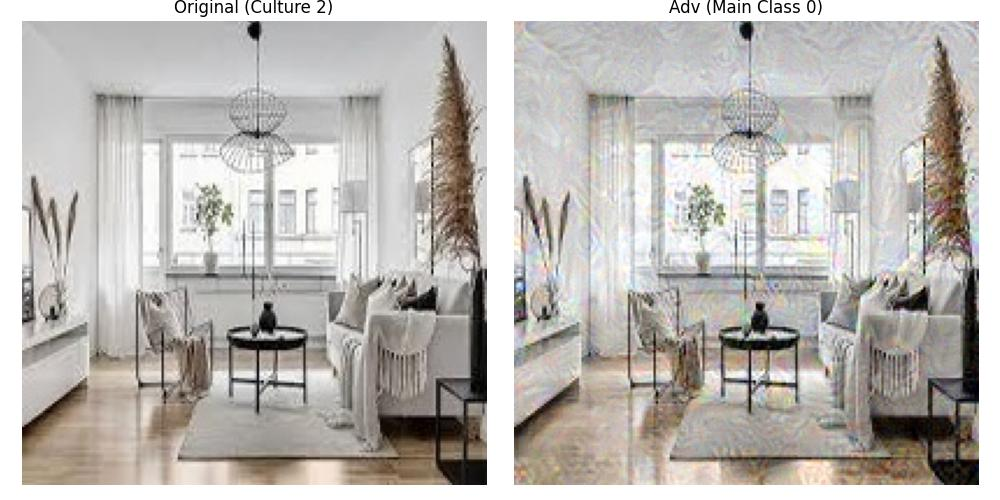
\includegraphics[width=\columnwidth]{adv_gen_figures/adv_rt_CI_CLSDIV0_source2.jpg}
\end{subfigure} 
\caption{Example of transformations applied on Ind. Jap. and Scan. dataset with with carpets using PGD, RT and CLSDIV with Ind. as majority culture.}
\label{fig::advrtCI_CLSDIV0}
\end{figure}

\begin{figure}[H]
\centering
\begin{subfigure}[b]{0.6\columnwidth}
\centering
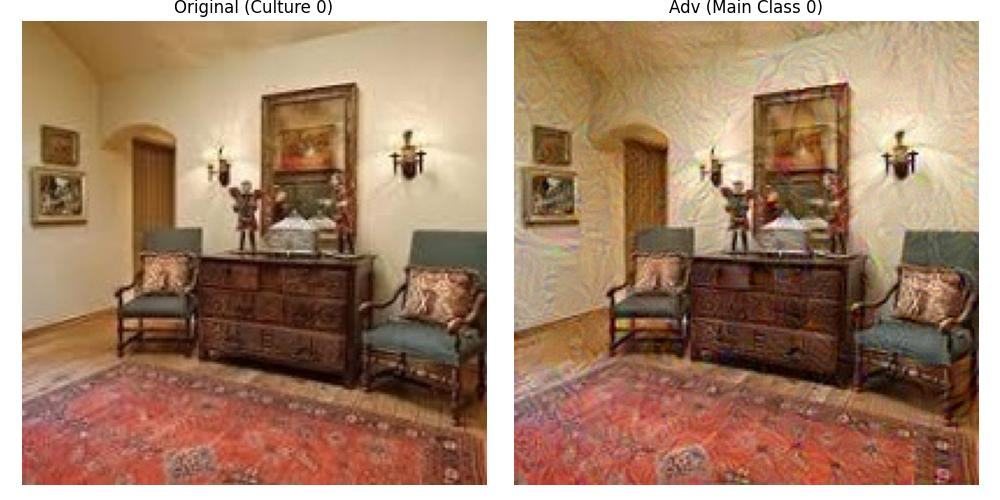
\includegraphics[width=\columnwidth]{adv_gen_figures/adv_rt_CJ_CLSDIV0_source0.jpg}

\end{subfigure} \\
\begin{subfigure}[b]{0.6\columnwidth}
\centering
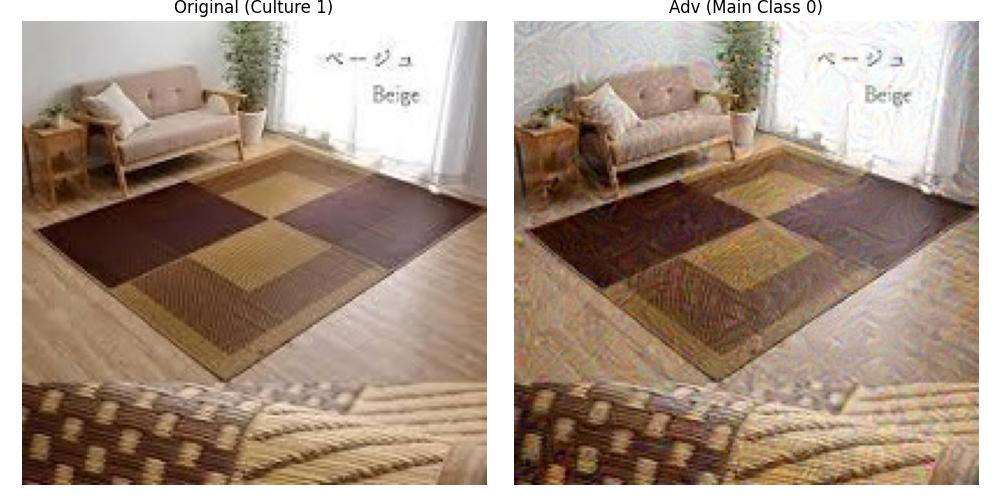
\includegraphics[width=\columnwidth]{adv_gen_figures/adv_rt_CJ_CLSDIV0_source1.jpg}
\end{subfigure} \\
\begin{subfigure}[b]{0.6\columnwidth}
\centering
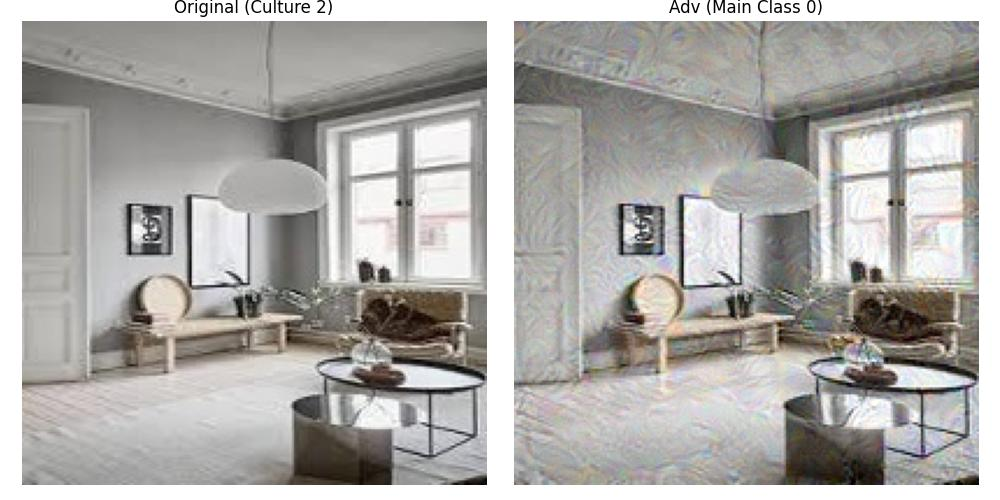
\includegraphics[width=\columnwidth]{adv_gen_figures/adv_rt_CJ_CLSDIV0_source2.jpg}
\end{subfigure} 
\caption{Example of transformations applied on Ind. Jap. and Scan. dataset with with carpets using PGD, RT and CLSDIV with Jap. as majority culture.}
\label{fig::advrtCJ_CLSDIV0}
\end{figure}

\begin{figure}[H]
\centering
\begin{subfigure}[b]{0.6\columnwidth}
\centering
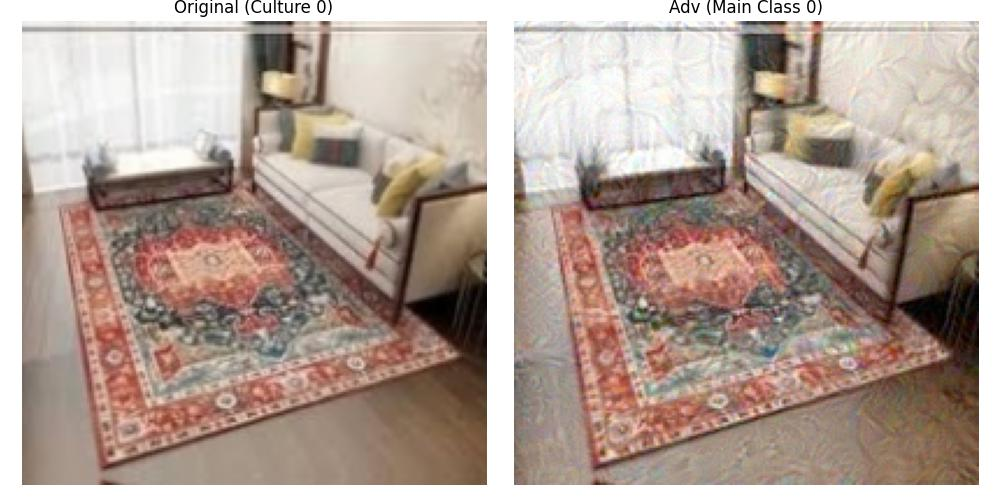
\includegraphics[width=\columnwidth]{adv_gen_figures/adv_rt_CS_CLSDIV0_source0.jpg}
\end{subfigure} \\
\begin{subfigure}[b]{0.6\columnwidth}
\centering
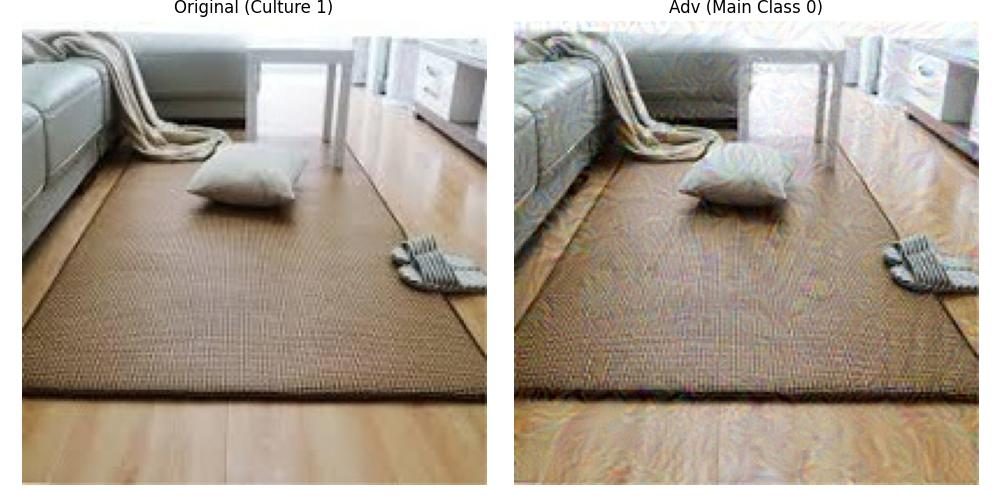
\includegraphics[width=\columnwidth]{adv_gen_figures/adv_rt_CS_CLSDIV0_source1.jpg}
\end{subfigure} \\
\begin{subfigure}[b]{0.6\columnwidth}
\centering
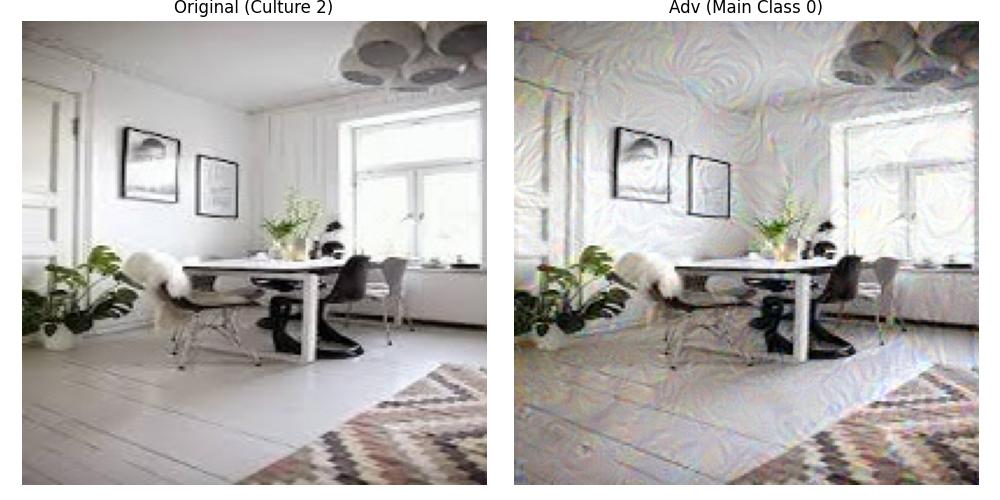
\includegraphics[width=\columnwidth]{adv_gen_figures/adv_rt_CS_CLSDIV0_source2.jpg}
\end{subfigure} 
\caption{Example of transformations applied on Ind. Jap. and Scan. dataset with with carpets using PGD, RT and CLSDIV with Scan. as majority culture.}
\label{fig::advrtCS_CLSDIV0}
\end{figure}

%CLSDIV 1
\begin{figure}[H]
\centering
\begin{subfigure}[b]{0.6\columnwidth}
\centering
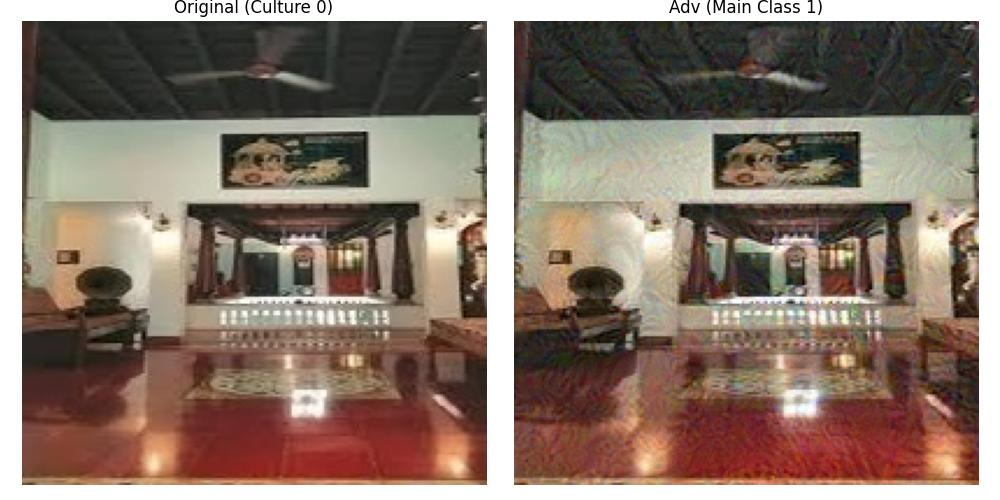
\includegraphics[width=\columnwidth]{adv_gen_figures/adv_rt_CI_CLSDIV1_source0.jpg}
\end{subfigure} \\
\begin{subfigure}[b]{0.6\columnwidth}
\centering
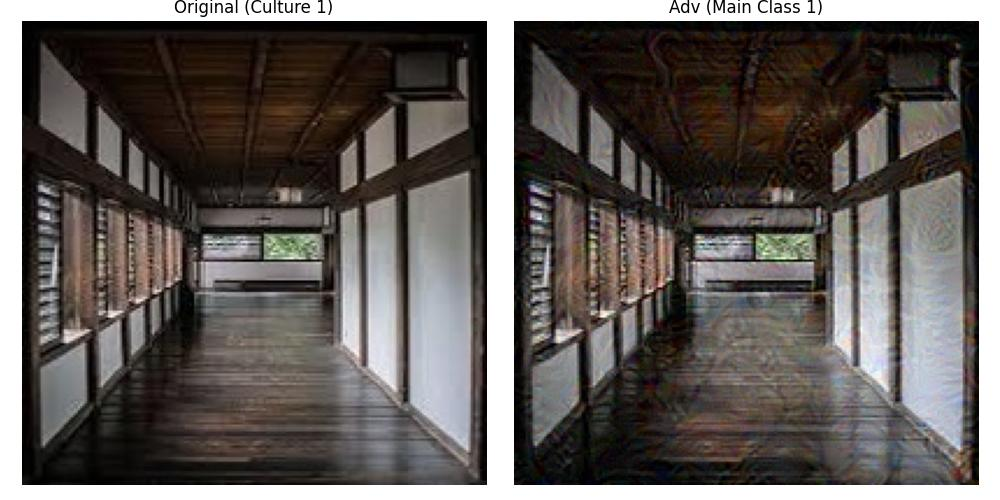
\includegraphics[width=\columnwidth]{adv_gen_figures/adv_rt_CI_CLSDIV1_source1.jpg}
\end{subfigure} \\
\begin{subfigure}[b]{0.6\columnwidth}
\centering
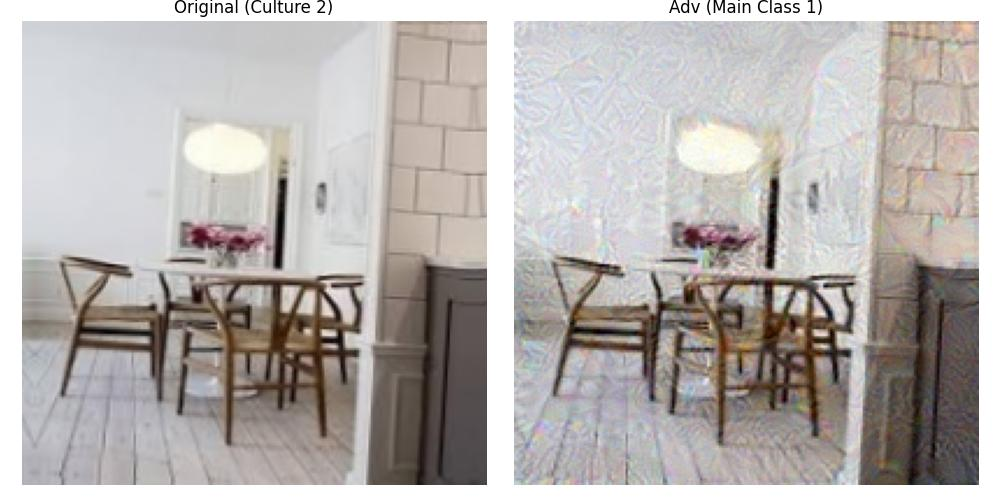
\includegraphics[width=\columnwidth]{adv_gen_figures/adv_rt_CI_CLSDIV1_source2.jpg}
\end{subfigure} 
\caption{Example of transformations applied on Ind. Jap. and Scan. dataset without carpets using PGD, RT and CLSDIV with Ind. as majority culture.}
\label{fig::advrtCI_CLSDIV1}
\end{figure}

\begin{figure}[H]
\centering
\begin{subfigure}[b]{0.6\columnwidth}
\centering
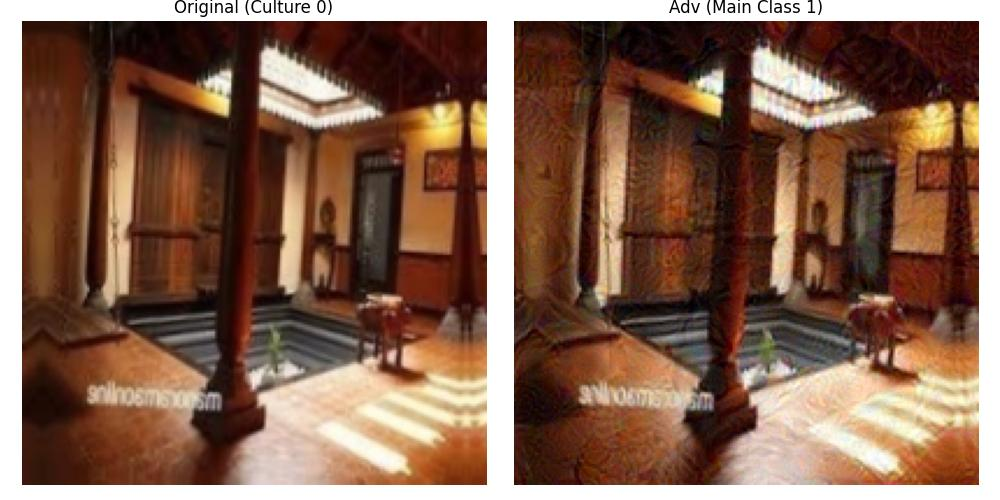
\includegraphics[width=\columnwidth]{adv_gen_figures/adv_rt_CJ_CLSDIV1_source0.jpg}
\end{subfigure} \\
\begin{subfigure}[b]{0.6\columnwidth}
\centering
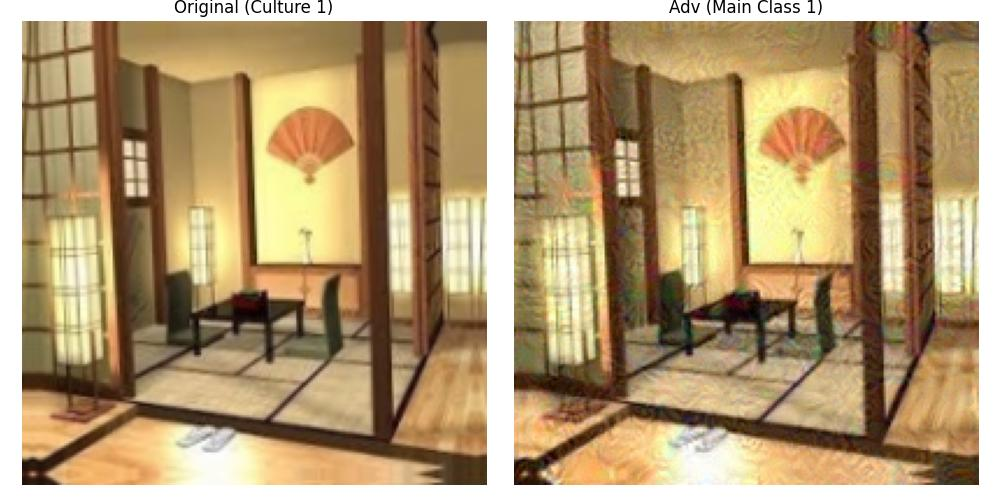
\includegraphics[width=\columnwidth]{adv_gen_figures/adv_rt_CJ_CLSDIV1_source1.jpg}
\end{subfigure} \\
\begin{subfigure}[b]{0.6\columnwidth}
\centering
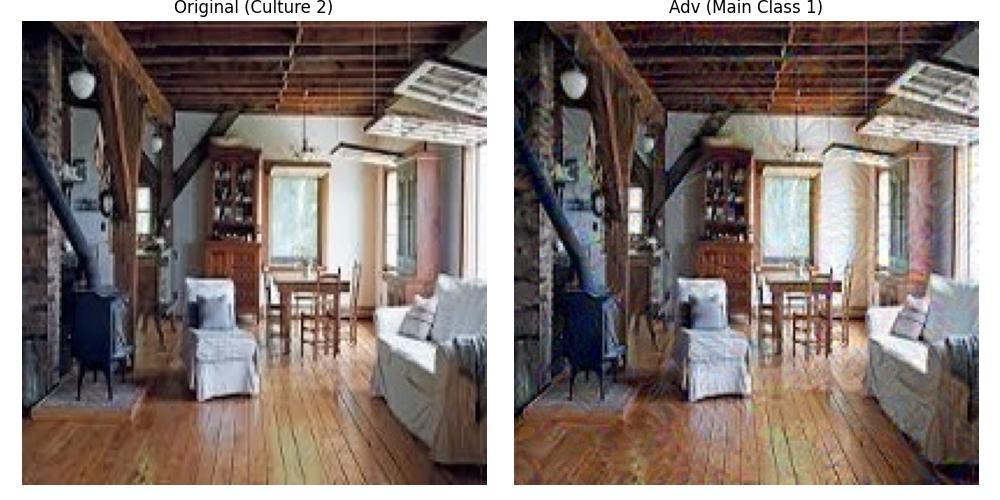
\includegraphics[width=\columnwidth]{adv_gen_figures/adv_rt_CJ_CLSDIV1_source2.jpg}
\end{subfigure} 
\caption{Example of transformations applied on Ind. Jap. and Scan. dataset without carpets using PGD, RT and CLSDIV with Jap. as majority culture.}
\label{fig::advrtCJ_CLSDIV1}
\end{figure}

\begin{figure}[H]
\centering
\begin{subfigure}[b]{0.6\columnwidth}
\centering
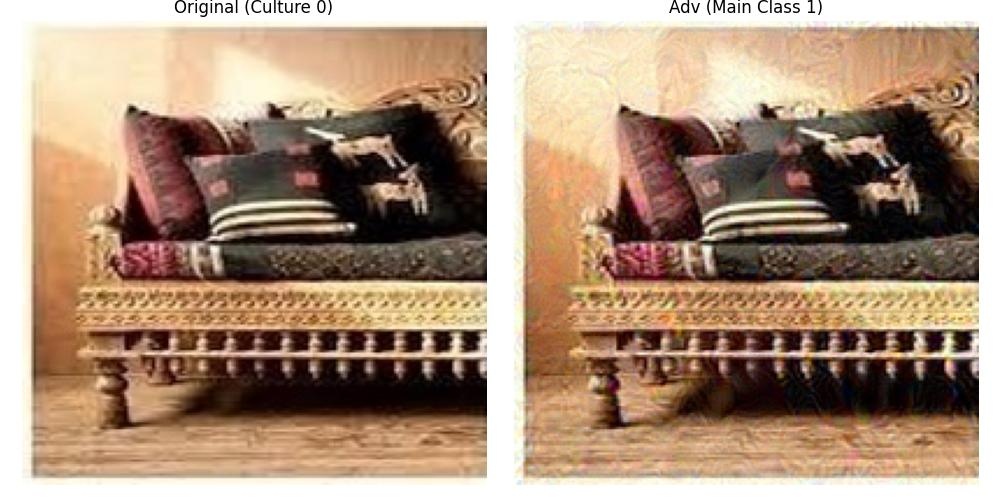
\includegraphics[width=\columnwidth]{adv_gen_figures/adv_rt_CS_CLSDIV1_source0.jpg}
\end{subfigure} \\
\begin{subfigure}[b]{0.6\columnwidth}
\centering
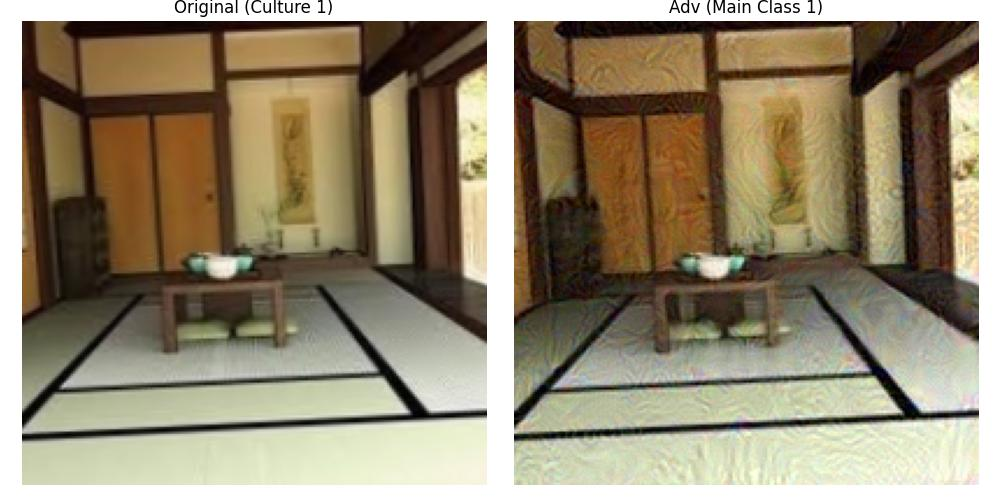
\includegraphics[width=\columnwidth]{adv_gen_figures/adv_rt_CS_CLSDIV1_source1.jpg}
\end{subfigure} \\
\begin{subfigure}[b]{0.6\columnwidth}
\centering
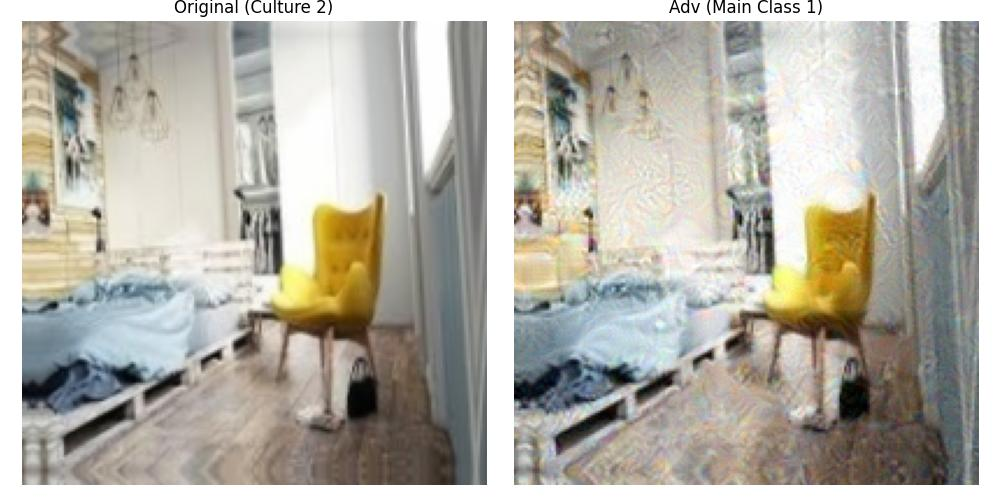
\includegraphics[width=\columnwidth]{adv_gen_figures/adv_rt_CS_CLSDIV1_source2.jpg}
\end{subfigure} 
\caption{Example of transformations applied on Ind. Jap. and Scan. dataset without carpets using PGD, RT and CLSDIV with Scan. as majority culture.}
\label{fig::advrtCS_CLSDIV1}
\end{figure}

% NOCLSDIV 0
\begin{figure}[H]
\centering
\begin{subfigure}[b]{0.6\columnwidth}
\centering
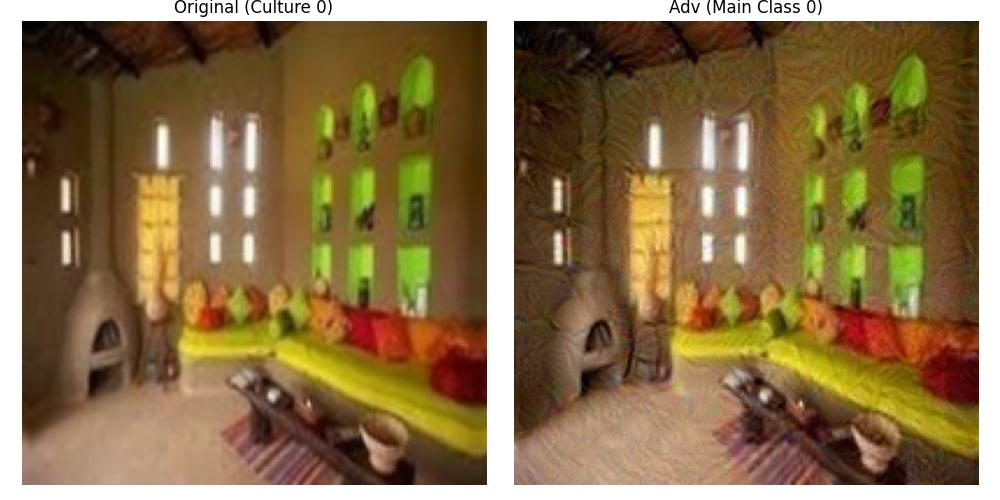
\includegraphics[width=\columnwidth]{adv_gen_figures/adv_rt_CI_NOCLSDIV0_source0.jpg}
\end{subfigure} \\
\begin{subfigure}[b]{0.6\columnwidth}
\centering
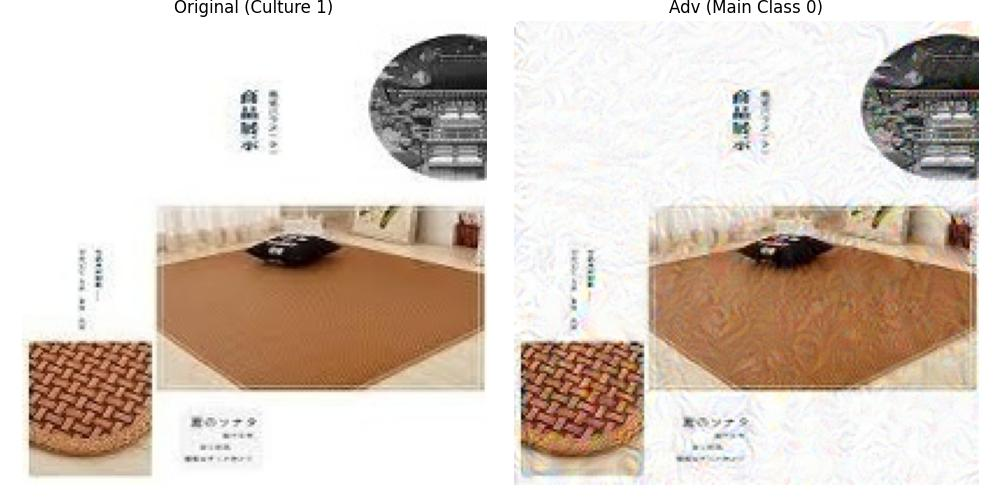
\includegraphics[width=\columnwidth]{adv_gen_figures/adv_rt_CI_NOCLSDIV0_source1.jpg}
\end{subfigure} \\
\begin{subfigure}[b]{0.6\columnwidth}
\centering
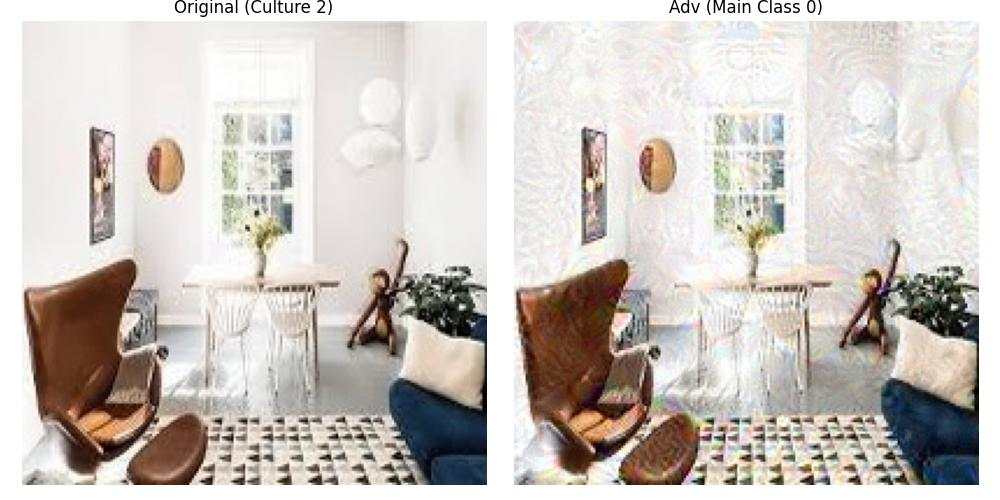
\includegraphics[width=\columnwidth]{adv_gen_figures/adv_rt_CI_NOCLSDIV0_source2.jpg}
\end{subfigure} 
\caption{Example of transformations applied on Ind. Jap. and Scan. dataset with with carpets using PGD, RT and NOCLSDIV with Ind. as majority culture.}
\label{fig::advrtCI_NOCLSDIV0}
\end{figure}

\begin{figure}[H]
\centering
\begin{subfigure}[b]{0.6\columnwidth}
\centering
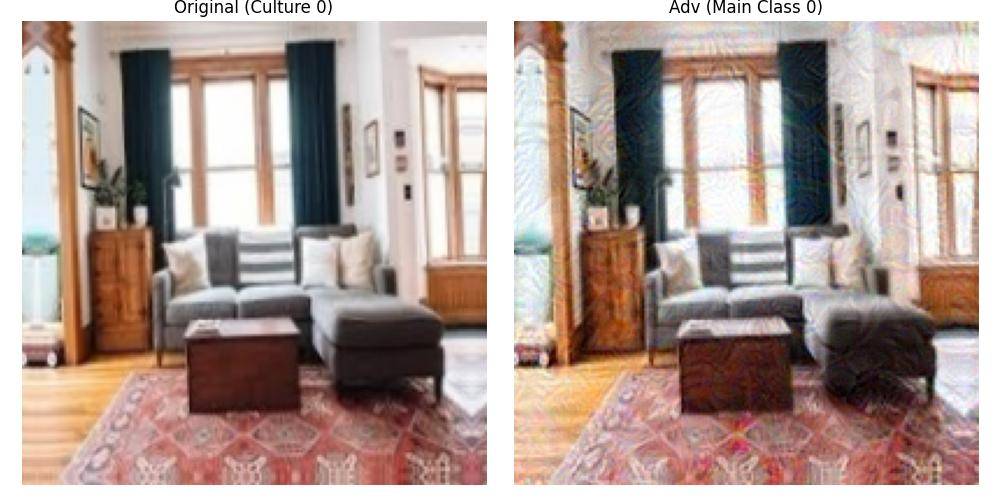
\includegraphics[width=\columnwidth]{adv_gen_figures/adv_rt_CJ_NOCLSDIV0_source0.jpg}
\end{subfigure} \\
\begin{subfigure}[b]{0.6\columnwidth}
\centering
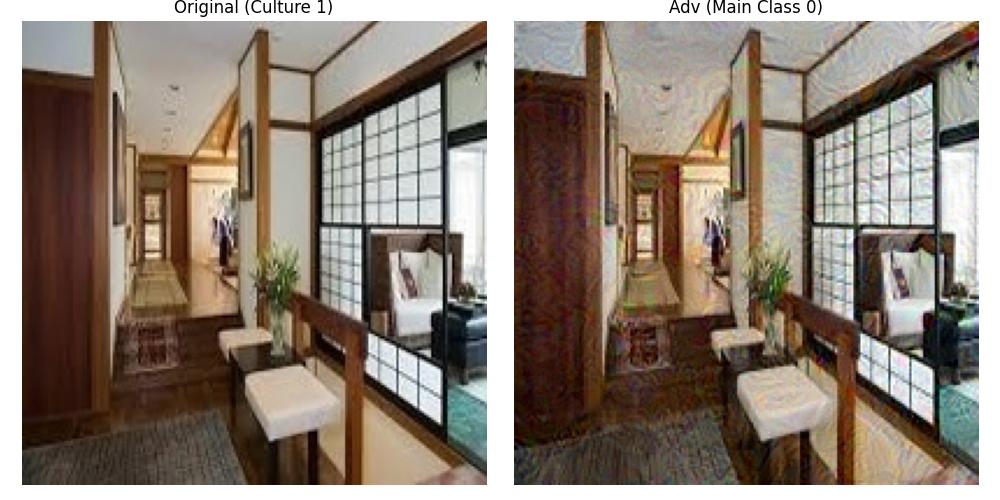
\includegraphics[width=\columnwidth]{adv_gen_figures/adv_rt_CJ_NOCLSDIV0_source1.jpg}
\end{subfigure} \\
\begin{subfigure}[b]{0.6\columnwidth}
\centering
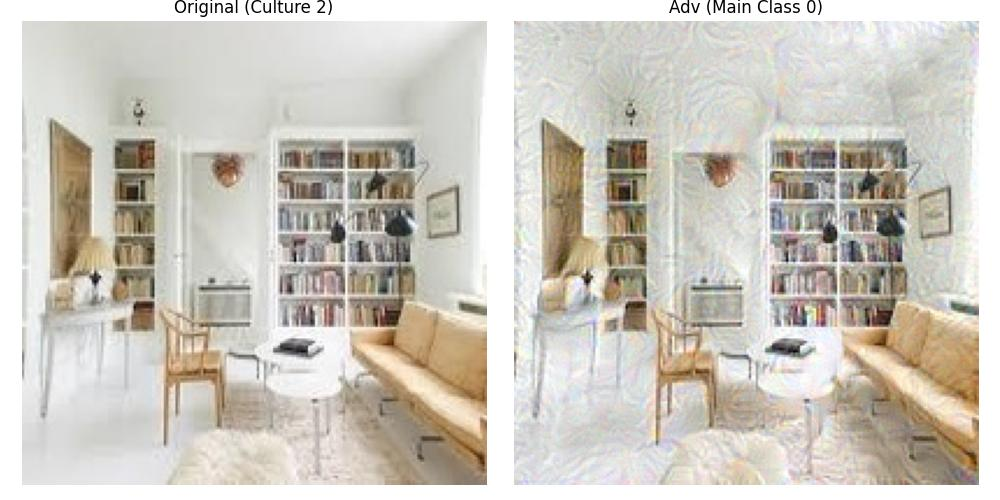
\includegraphics[width=\columnwidth]{adv_gen_figures/adv_rt_CJ_NOCLSDIV0_source2.jpg}
\end{subfigure} 
\caption{Example of transformations applied on Ind. Jap. and Scan. dataset with with carpets using PGD, RT and NOCLSDIV with Jap. as majority culture.}
\label{fig::advrtCJ_NOCLSDIV0}
\end{figure}

\begin{figure}[H]
\centering
\begin{subfigure}[b]{0.6\columnwidth}
\centering
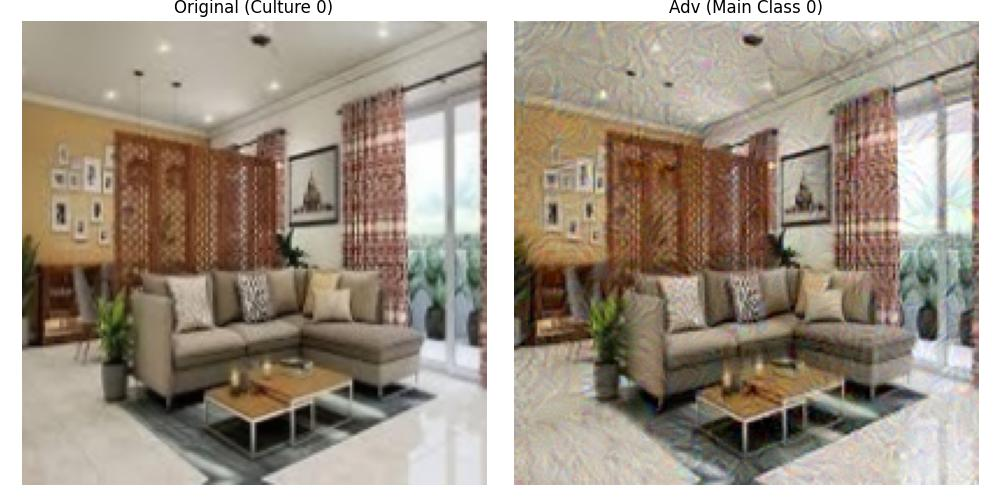
\includegraphics[width=\columnwidth]{adv_gen_figures/adv_rt_CS_NOCLSDIV0_source0.jpg}
\end{subfigure} \\
\begin{subfigure}[b]{0.6\columnwidth}
\centering
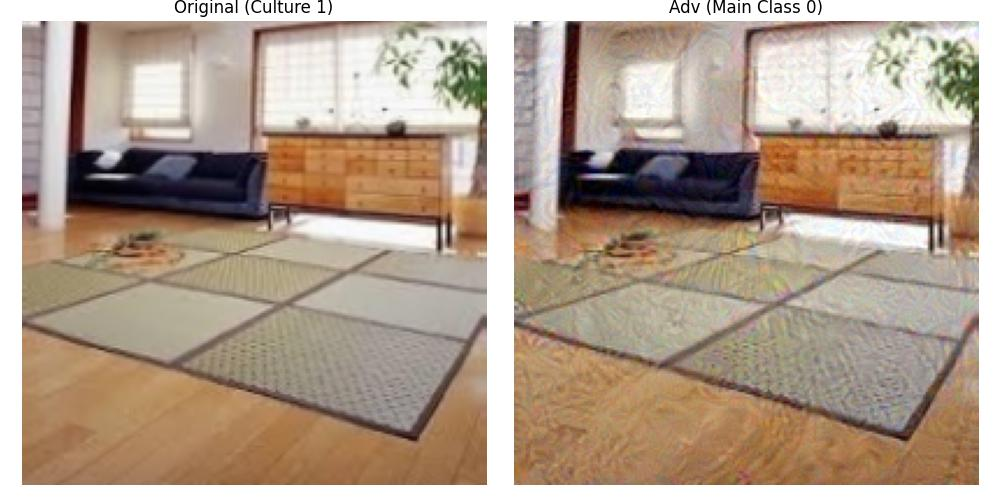
\includegraphics[width=\columnwidth]{adv_gen_figures/adv_rt_CS_NOCLSDIV0_source1.jpg}
\end{subfigure} \\
\begin{subfigure}[b]{0.6\columnwidth}
\centering
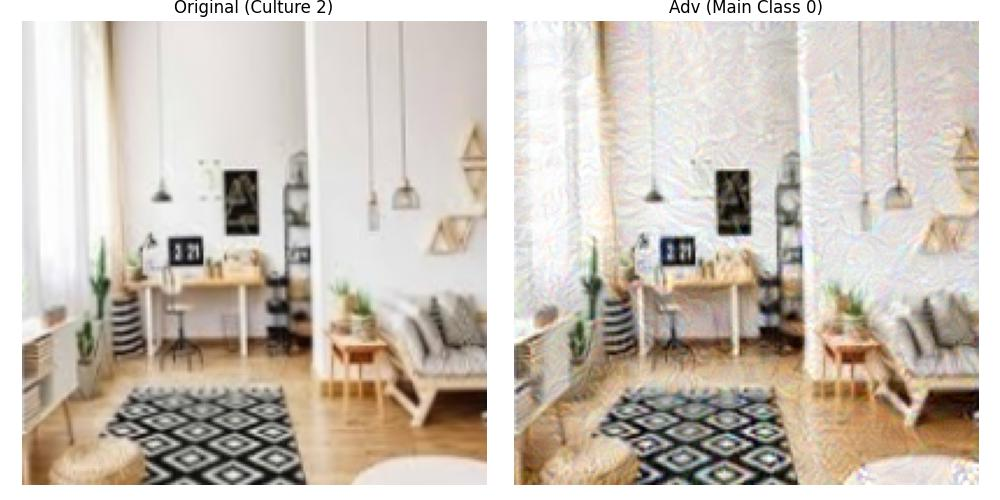
\includegraphics[width=\columnwidth]{adv_gen_figures/adv_rt_CS_NOCLSDIV0_source2.jpg}
\end{subfigure} 
\caption{Example of transformations applied on Ind. Jap. and Scan. dataset with with carpets using PGD, RT and NOCLSDIV with Scan. as majority culture.}
\label{fig::advrtCS_NOCLSDIV0}
\end{figure}

% NOCLSDIV 1
\begin{figure}[H]
\centering
\begin{subfigure}[b]{0.6\columnwidth}
\centering
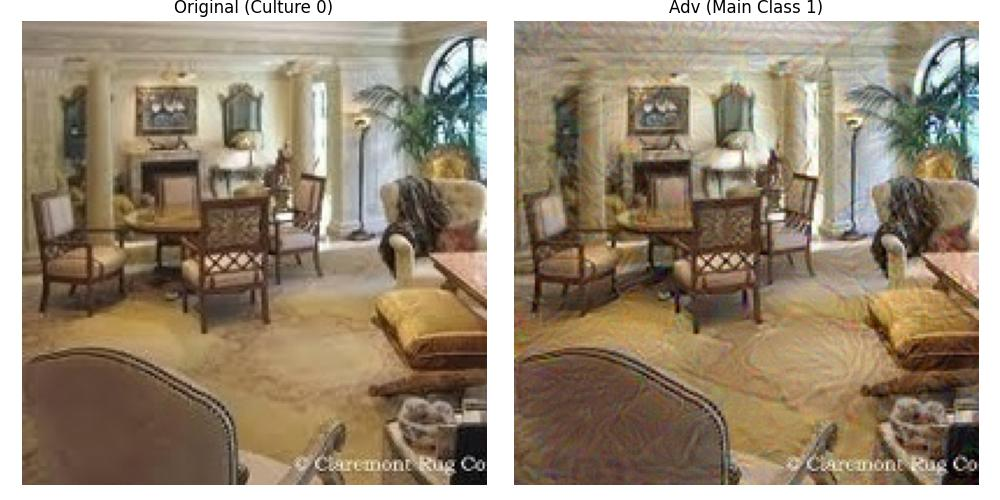
\includegraphics[width=\columnwidth]{adv_gen_figures/adv_rt_CI_NOCLSDIV1_source0.jpg}
\end{subfigure} \\
\begin{subfigure}[b]{0.6\columnwidth}
\centering
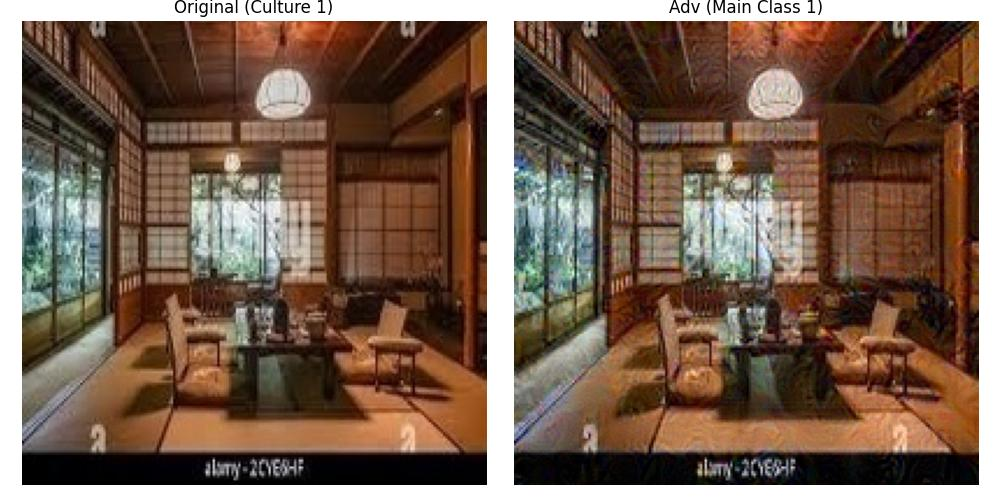
\includegraphics[width=\columnwidth]{adv_gen_figures/adv_rt_CI_NOCLSDIV1_source1.jpg}
\end{subfigure} \\
\begin{subfigure}[b]{0.6\columnwidth}
\centering
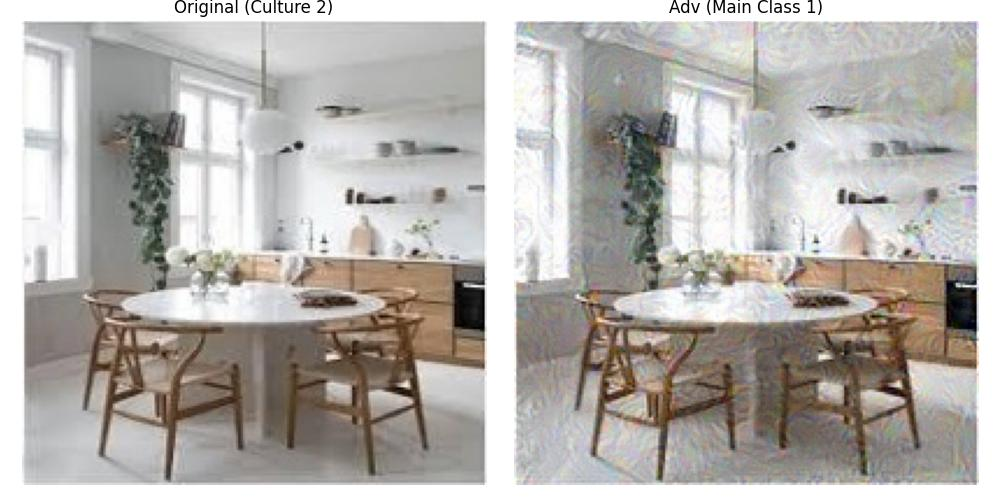
\includegraphics[width=\columnwidth]{adv_gen_figures/adv_rt_CI_NOCLSDIV1_source2.jpg}
\end{subfigure} 
\caption{Example of transformations applied on Ind. Jap. and Scan. dataset without carpets using PGD, RT and NOCLSDIV with Ind. as majority culture.}
\label{fig::advrtCI_NOCLSDIV1}
\end{figure}

\begin{figure}[H]
\centering
\begin{subfigure}[b]{0.6\columnwidth}
\centering
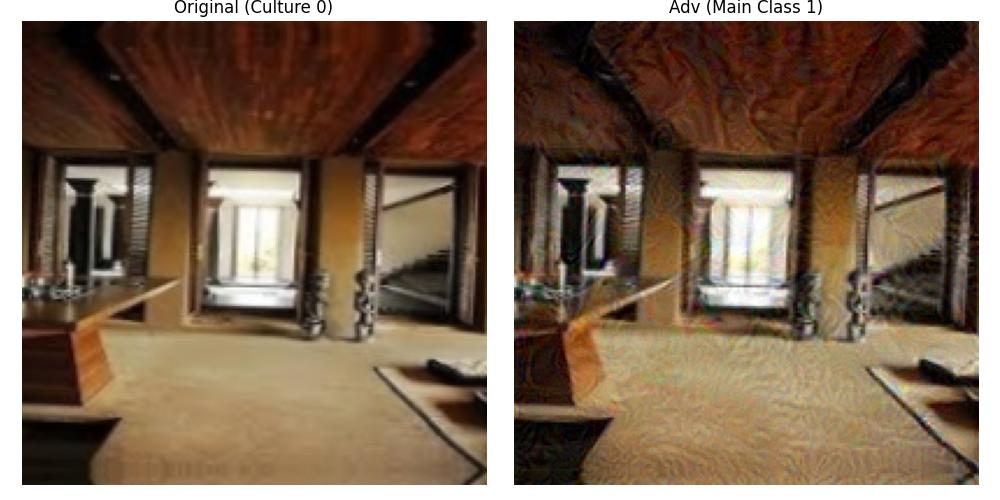
\includegraphics[width=\columnwidth]{adv_gen_figures/adv_rt_CJ_NOCLSDIV1_source0.jpg}
\end{subfigure} \\
\begin{subfigure}[b]{0.6\columnwidth}
\centering
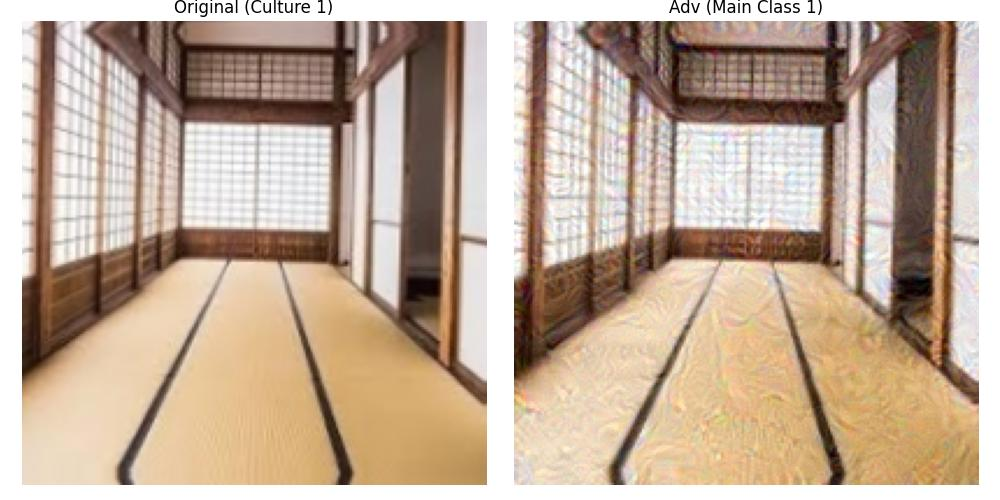
\includegraphics[width=\columnwidth]{adv_gen_figures/adv_rt_CJ_NOCLSDIV1_source1.jpg}
\end{subfigure} \\
\begin{subfigure}[b]{0.6\columnwidth}
\centering
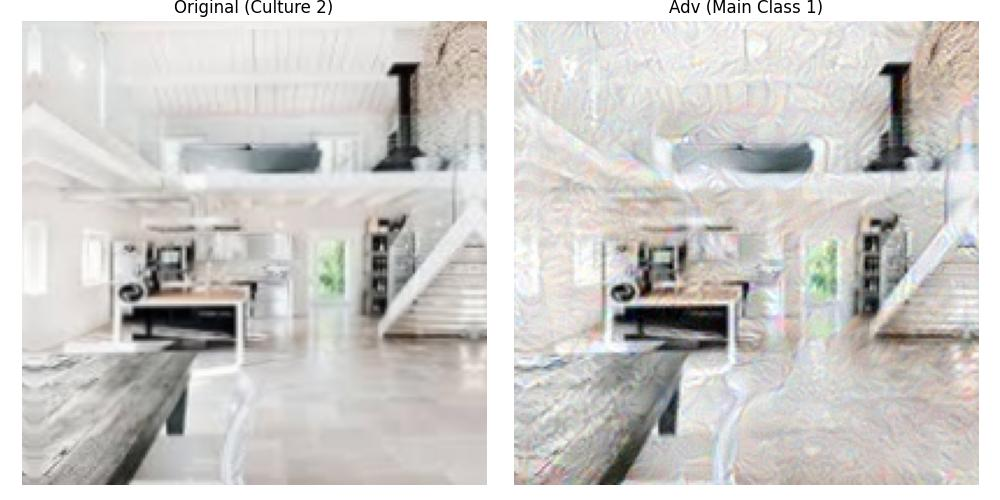
\includegraphics[width=\columnwidth]{adv_gen_figures/adv_rt_CJ_NOCLSDIV1_source2.jpg}
\end{subfigure} 
\caption{Example of transformations applied on Ind. Jap. and Scan. dataset without carpets using PGD, RT and NOCLSDIV with Jap. as majority culture.}
\label{fig::advrtCJ_NOCLSDIV1}
\end{figure}

\begin{figure}[H]
\centering
\begin{subfigure}[b]{0.6\columnwidth}
\centering
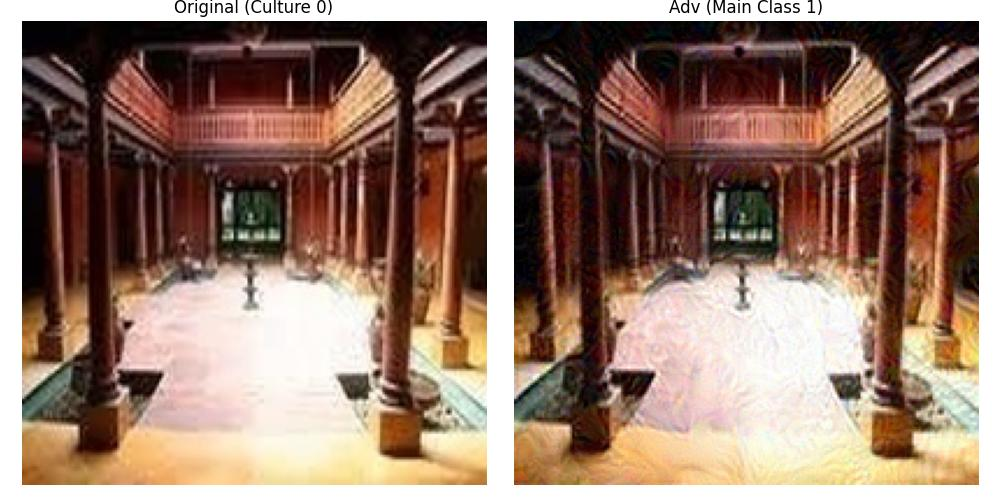
\includegraphics[width=\columnwidth]{adv_gen_figures/adv_rt_CS_NOCLSDIV1_source0.jpg}
\end{subfigure} \\
\begin{subfigure}[b]{0.6\columnwidth}
\centering
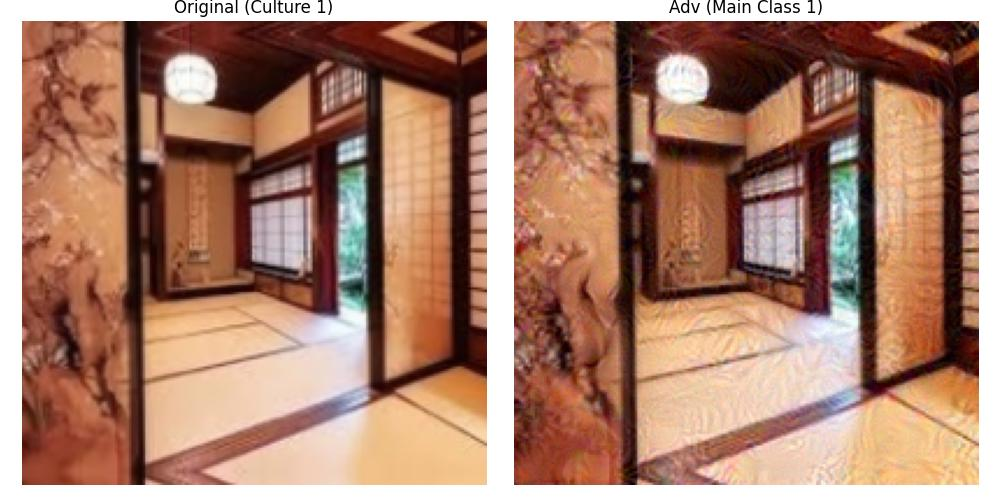
\includegraphics[width=\columnwidth]{adv_gen_figures/adv_rt_CS_NOCLSDIV1_source1.jpg}
\end{subfigure} \\
\begin{subfigure}[b]{0.6\columnwidth}
\centering
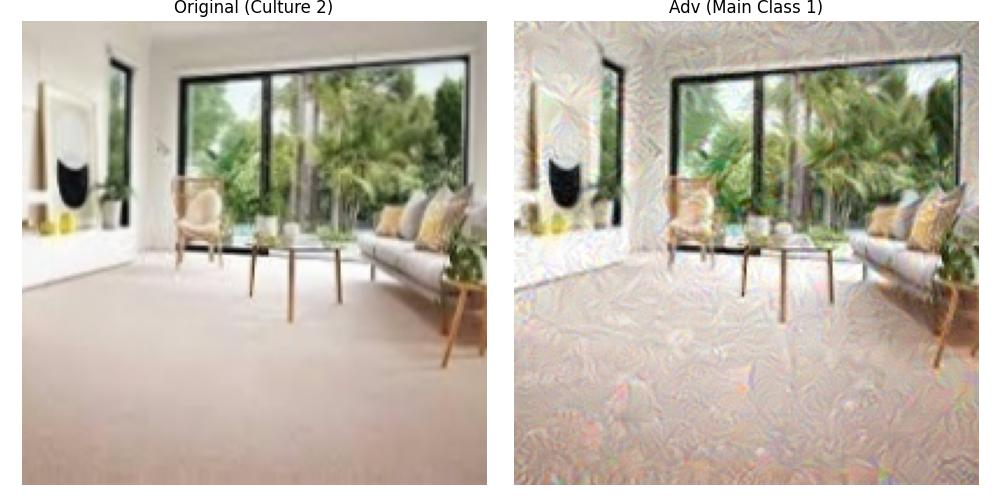
\includegraphics[width=\columnwidth]{adv_gen_figures/adv_rt_CS_NOCLSDIV1_source2.jpg}
\end{subfigure} 
\caption{Example of transformations applied on Ind. Jap. and Scan. dataset without carpets using PGD, RT and NOCLSDIV with Scan. as majority culture.}
\label{fig::advrtCS_NOCLSDIV1}
\end{figure}


% 0.2
Tables~\ref{fig::adv02LC_CLSDIV0}, \ref{fig::adv02LC_CLSDIV1}, \ref{fig::adv02LC_NOCLSDIV0}, \ref{fig::adv02LC_NOCLSDIV1}, \ref{fig::adv02LF_CLSDIV0}, \ref{fig::adv02LF_CLSDIV1}, \ref{fig::adv02LF_NOCLSDIV0}, \ref{fig::adv02LF_NOCLSDIV1},
\ref{fig::adv02LT_CLSDIV0}, \ref{fig::adv02LT_CLSDIV1}, \ref{fig::adv02LT_NOCLSDIV0}, \ref{fig::adv02LT_NOCLSDIV1} show examples of transformations applied on Chin., Fren. and Turk. images from LAMP dataset with lamps turned off using PGD, and CLSDIV or NOCLSDIV with Chin., Fren. and Turk as majority cultures with $p_u=20\%$.
%CLSDIV 0
\begin{figure}[H]
\centering
\begin{subfigure}[b]{0.6\columnwidth}
\centering
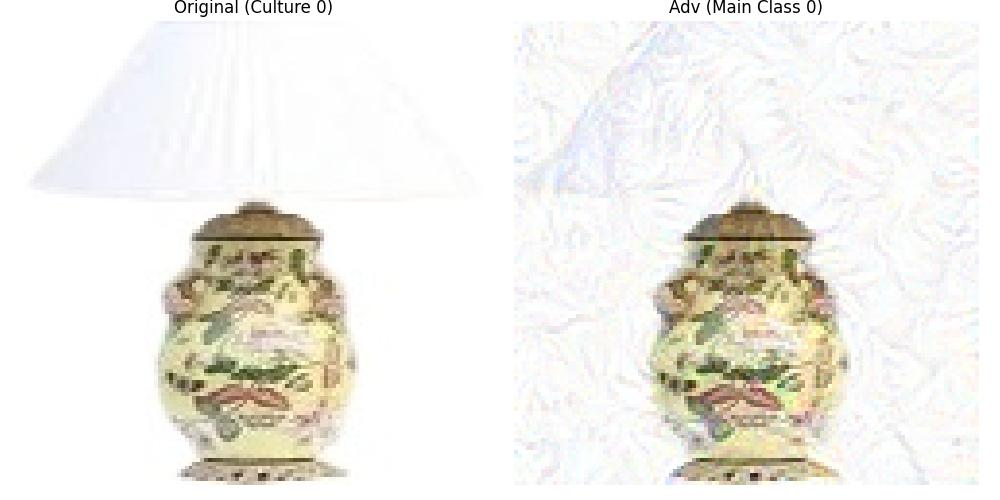
\includegraphics[width=\columnwidth]{adv_gen_figures/adv_02_majLC_CLSDIV0_source0.jpg}
\end{subfigure} \\
\begin{subfigure}[b]{0.6\columnwidth}
\centering
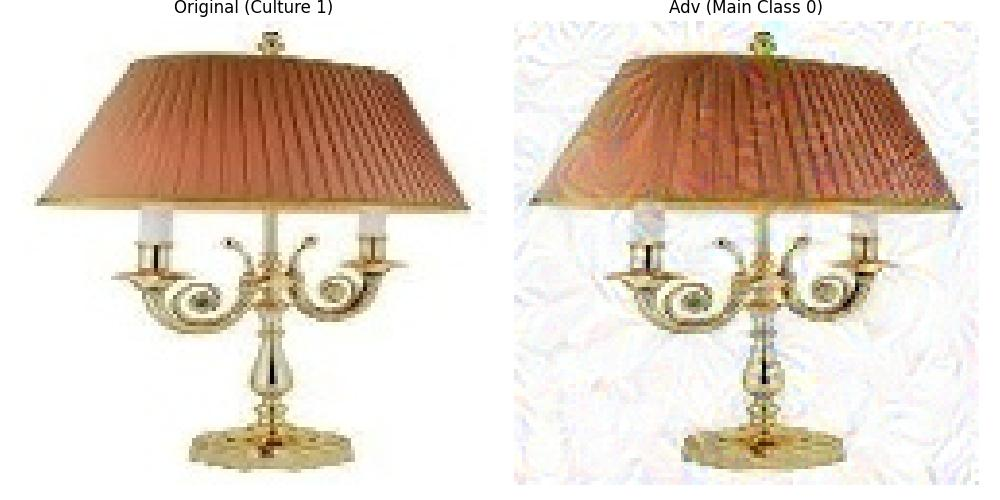
\includegraphics[width=\columnwidth]{adv_gen_figures/adv_02_majLC_CLSDIV0_source1.jpg}
\end{subfigure} \\
\begin{subfigure}[b]{0.6\columnwidth}
\centering
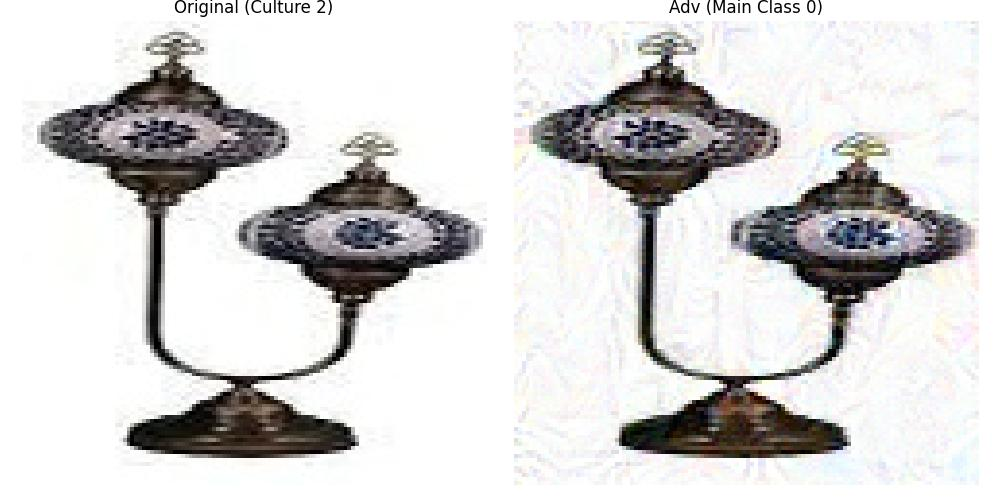
\includegraphics[width=\columnwidth]{adv_gen_figures/adv_02_majLC_CLSDIV0_source2.jpg}
\end{subfigure}
\caption{Example of transformations applied on Chin., Fren. and Turk. images from LAMP dataset with lamps turned off using PGD and CLSDIV with Chin. as majority culture.}
\label{fig::adv02LC_CLSDIV0}
\end{figure}

\begin{figure}[H]
\centering
\begin{subfigure}[b]{0.6\columnwidth}
\centering
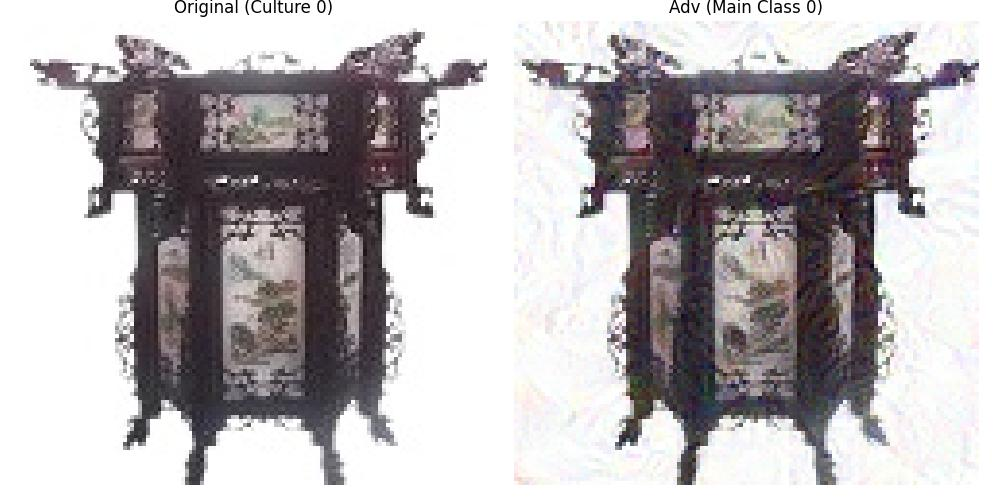
\includegraphics[width=\columnwidth]{adv_gen_figures/adv_02_majLF_CLSDIV0_source0.jpg}

\end{subfigure} \\
\begin{subfigure}[b]{0.6\columnwidth}
\centering
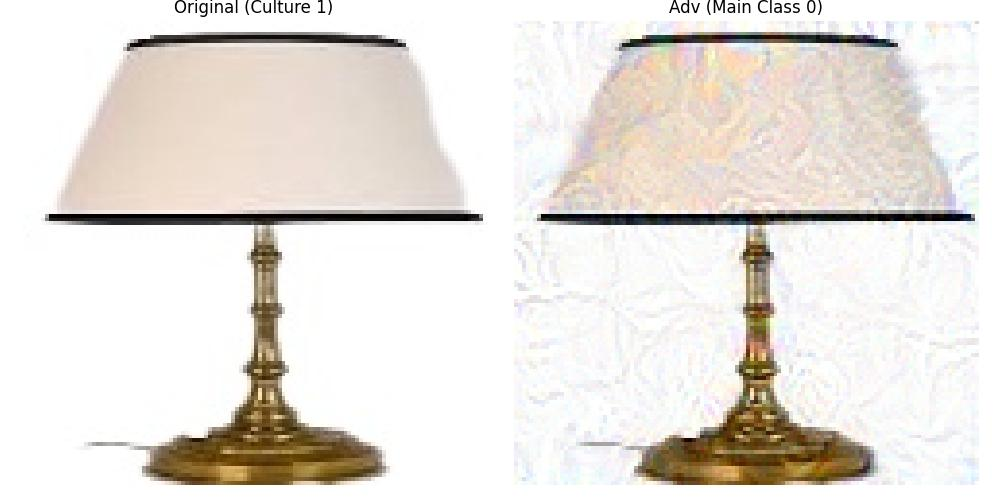
\includegraphics[width=\columnwidth]{adv_gen_figures/adv_02_majLF_CLSDIV0_source1.jpg}
\end{subfigure} \\
\begin{subfigure}[b]{0.6\columnwidth}
\centering
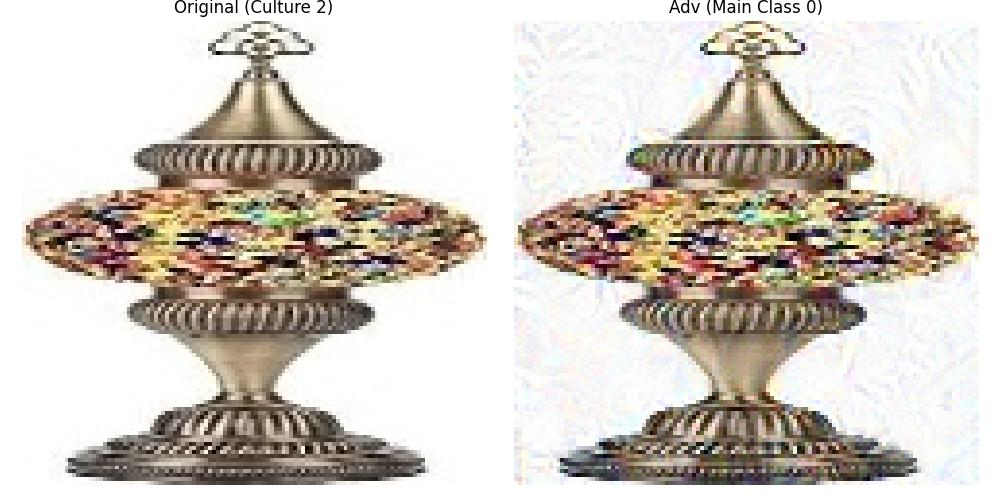
\includegraphics[width=\columnwidth]{adv_gen_figures/adv_02_majLF_CLSDIV0_source2.jpg}
\end{subfigure} 
\caption{Example of transformations applied on Chin., Fren. and Turk. images from LAMP dataset with lamps turned off using PGD and CLSDIV with Fren. as majority culture.}
\label{fig::adv02LF_CLSDIV0}
\end{figure}

\begin{figure}[H]
\centering
\begin{subfigure}[b]{0.6\columnwidth}
\centering
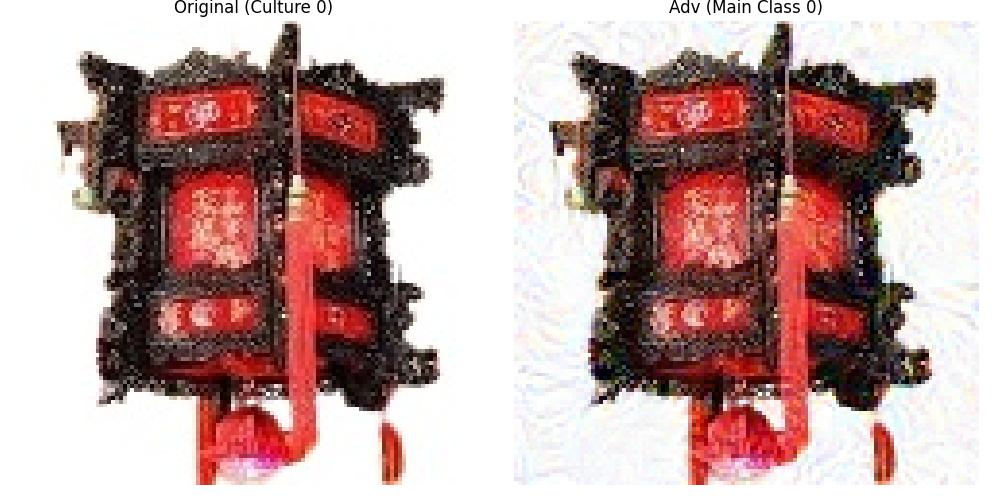
\includegraphics[width=\columnwidth]{adv_gen_figures/adv_02_majLT_CLSDIV0_source0.jpg}
\end{subfigure} \\
\begin{subfigure}[b]{0.6\columnwidth}
\centering
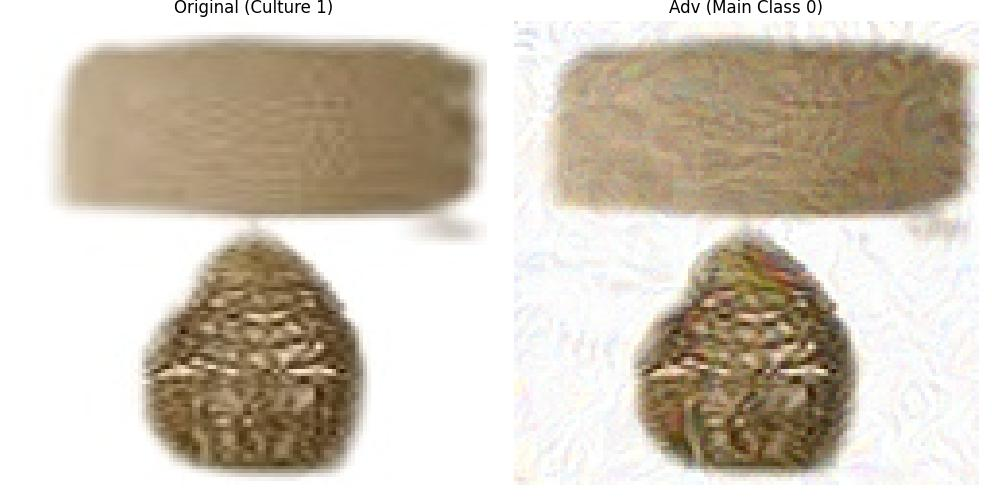
\includegraphics[width=\columnwidth]{adv_gen_figures/adv_02_majLT_CLSDIV0_source1.jpg}
\end{subfigure} \\
\begin{subfigure}[b]{0.6\columnwidth}
\centering
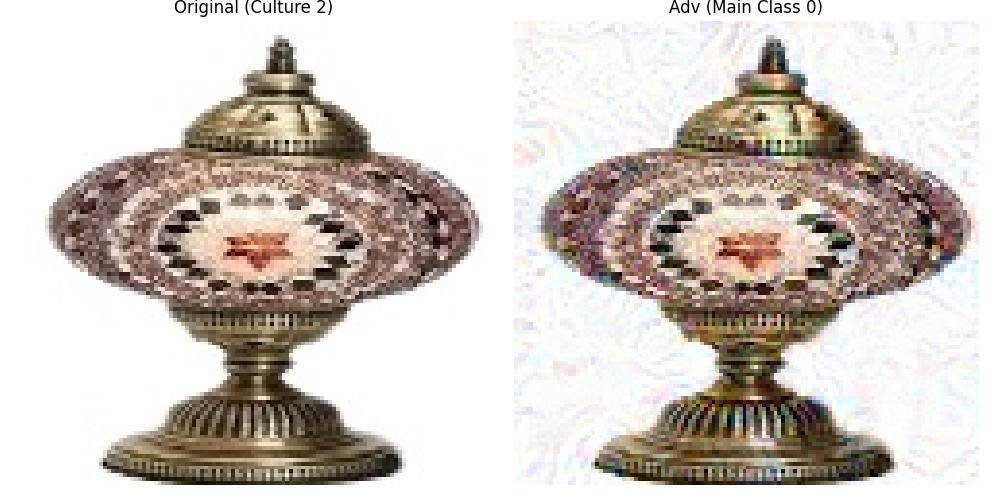
\includegraphics[width=\columnwidth]{adv_gen_figures/adv_02_majLT_CLSDIV0_source2.jpg}
\end{subfigure} 
\caption{Example of transformations applied on Chin., Fren. and Turk. images from LAMP dataset with lamps turned off using PGD and CLSDIV with Turk. as majority culture.}
\label{fig::adv02LT_CLSDIV0}
\end{figure}

%CLSDIV 1
\begin{figure}[H]
\centering
\begin{subfigure}[b]{0.6\columnwidth}
\centering
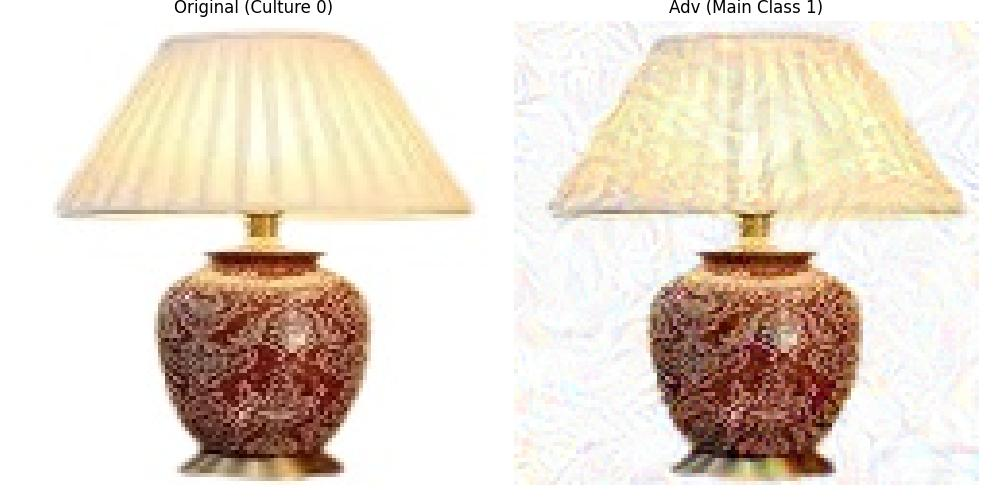
\includegraphics[width=\columnwidth]{adv_gen_figures/adv_02_majLC_CLSDIV1_source0.jpg}
\end{subfigure} \\
\begin{subfigure}[b]{0.6\columnwidth}
\centering
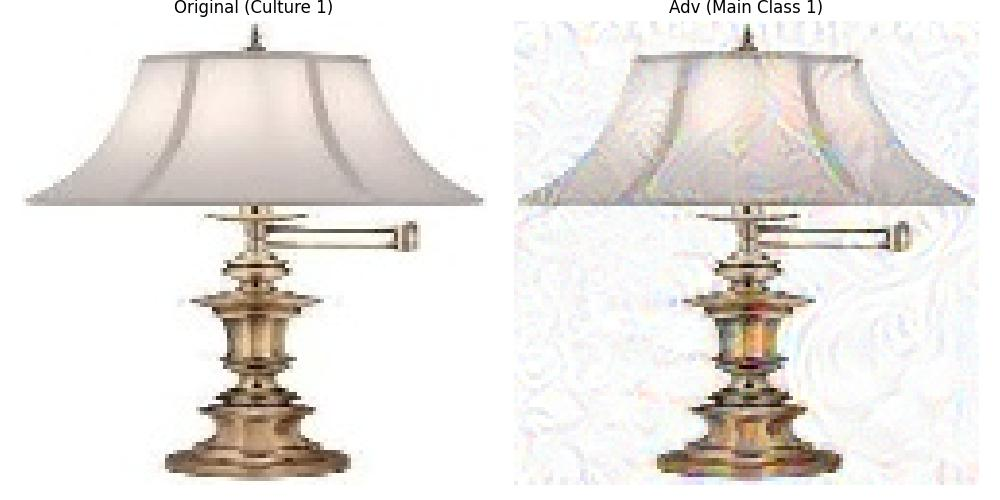
\includegraphics[width=\columnwidth]{adv_gen_figures/adv_02_majLC_CLSDIV1_source1.jpg}
\end{subfigure} \\
\begin{subfigure}[b]{0.6\columnwidth}
\centering
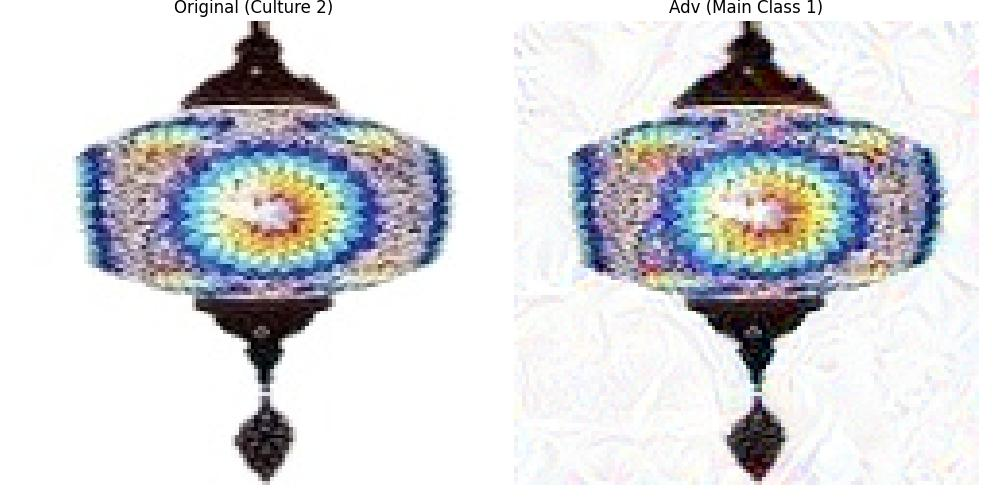
\includegraphics[width=\columnwidth]{adv_gen_figures/adv_02_majLC_CLSDIV1_source2.jpg}
\end{subfigure} 
\caption{Example of transformations applied on Chin., Fren. and Turk. images from LAMP dataset with lamps turned on using PGD and CLSDIV with Chin. as majority culture.}
\label{fig::adv02LC_CLSDIV1}
\end{figure}

\begin{figure}[H]
\centering
\begin{subfigure}[b]{0.6\columnwidth}
\centering
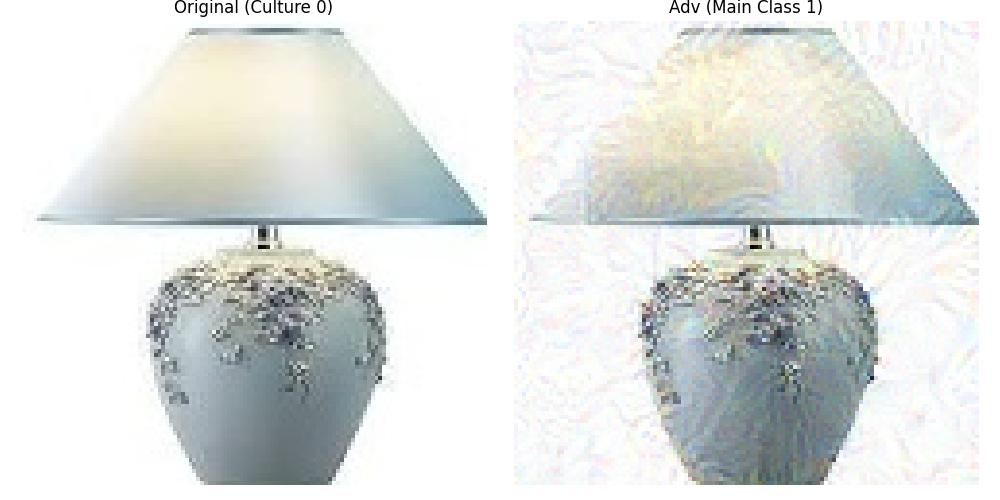
\includegraphics[width=\columnwidth]{adv_gen_figures/adv_02_majLF_CLSDIV1_source0.jpg}
\end{subfigure} \\
\begin{subfigure}[b]{0.6\columnwidth}
\centering
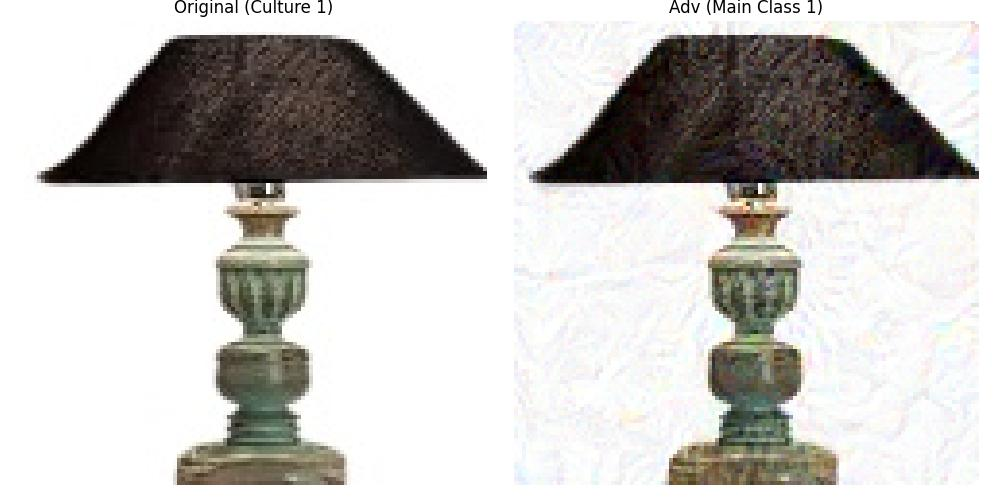
\includegraphics[width=\columnwidth]{adv_gen_figures/adv_02_majLF_CLSDIV1_source1.jpg}
\end{subfigure} \\
\begin{subfigure}[b]{0.6\columnwidth}
\centering
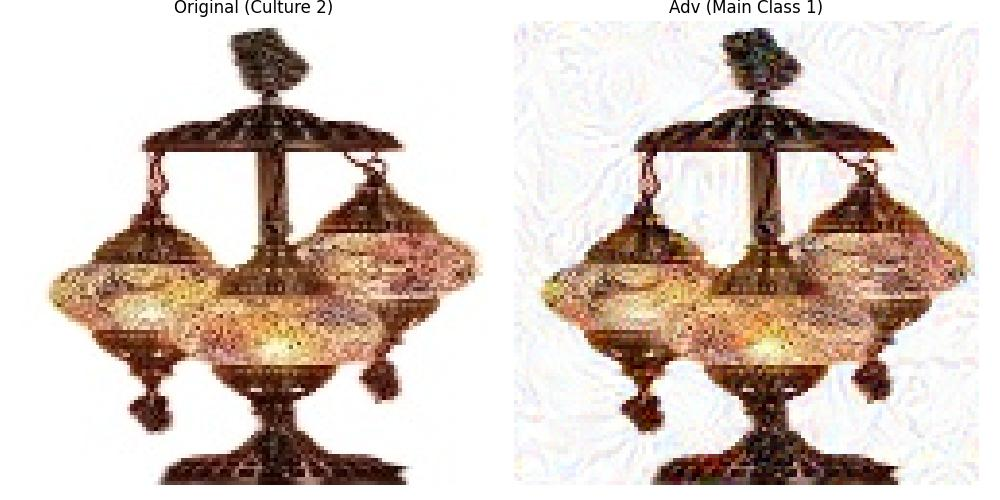
\includegraphics[width=\columnwidth]{adv_gen_figures/adv_02_majLF_CLSDIV1_source2.jpg}
\end{subfigure} 
\caption{Example of transformations applied on Chin., Fren. and Turk. images from LAMP dataset with lamps turned on using PGD and CLSDIV with Fren. as majority culture.}
\label{fig::adv02LF_CLSDIV1}
\end{figure}

\begin{figure}[H]
\centering
\begin{subfigure}[b]{0.6\columnwidth}
\centering
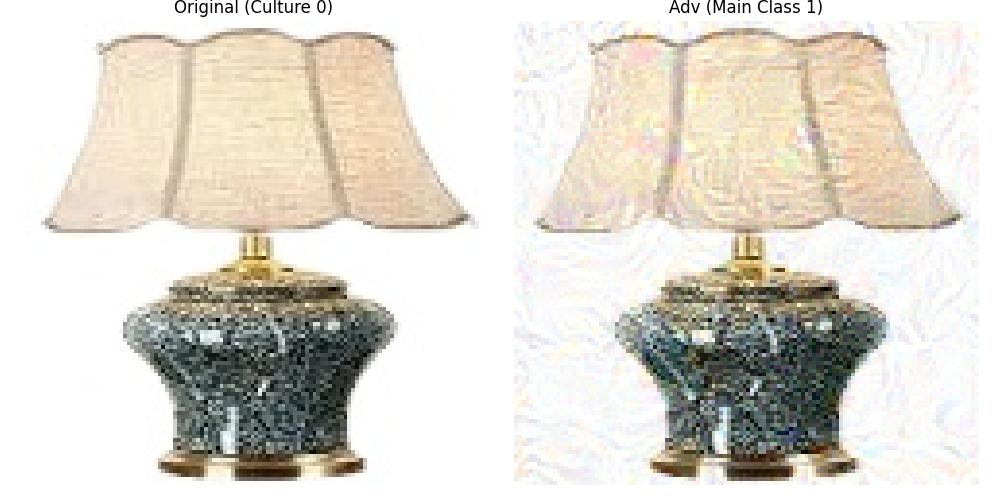
\includegraphics[width=\columnwidth]{adv_gen_figures/adv_02_majLT_CLSDIV1_source0.jpg}
\end{subfigure} \\
\begin{subfigure}[b]{0.6\columnwidth}
\centering
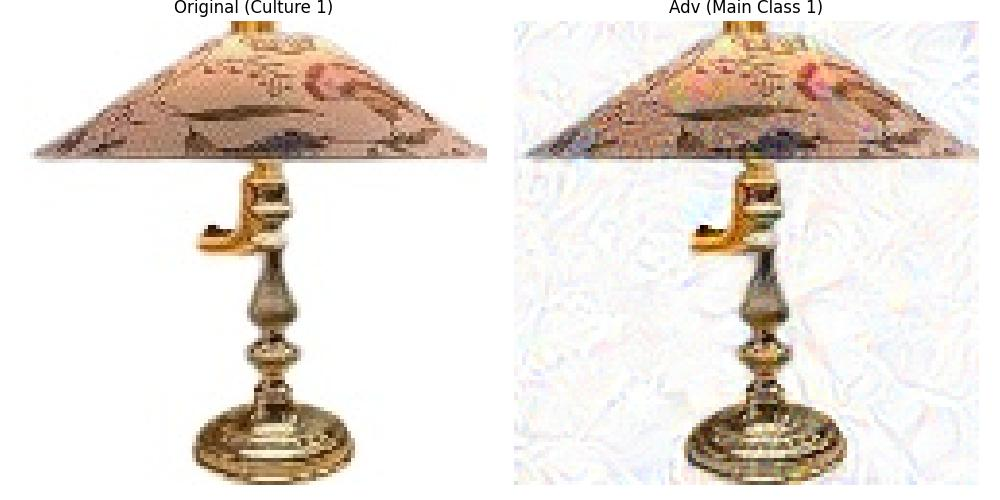
\includegraphics[width=\columnwidth]{adv_gen_figures/adv_02_majLT_CLSDIV1_source1.jpg}
\end{subfigure} \\
\begin{subfigure}[b]{0.6\columnwidth}
\centering
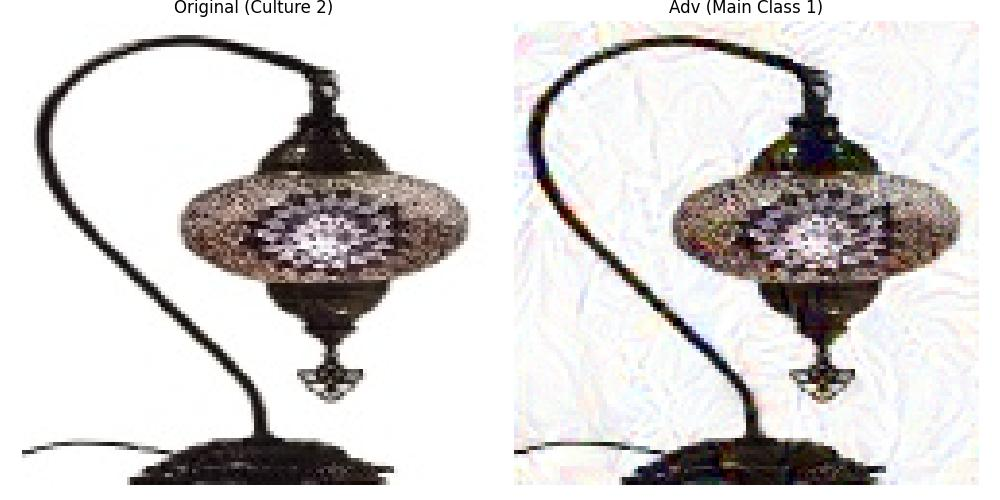
\includegraphics[width=\columnwidth]{adv_gen_figures/adv_02_majLT_CLSDIV1_source2.jpg}
\end{subfigure} 
\caption{Example of transformations applied on Chin., Fren. and Turk. images from LAMP dataset with lamps turned on using PGD and CLSDIV with Turk. as majority culture.}
\label{fig::adv02LT_CLSDIV1}
\end{figure}

% NOCLSDIV 0
\begin{figure}[H]
\centering
\begin{subfigure}[b]{0.6\columnwidth}
\centering
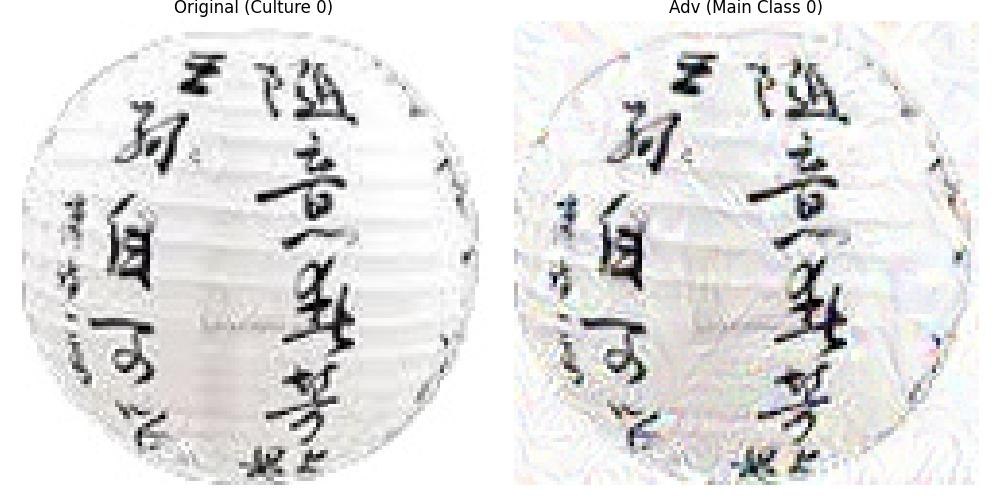
\includegraphics[width=\columnwidth]{adv_gen_figures/adv_02_majLC_NOCLSDIV0_source0.jpg}
\end{subfigure} \\
\begin{subfigure}[b]{0.6\columnwidth}
\centering
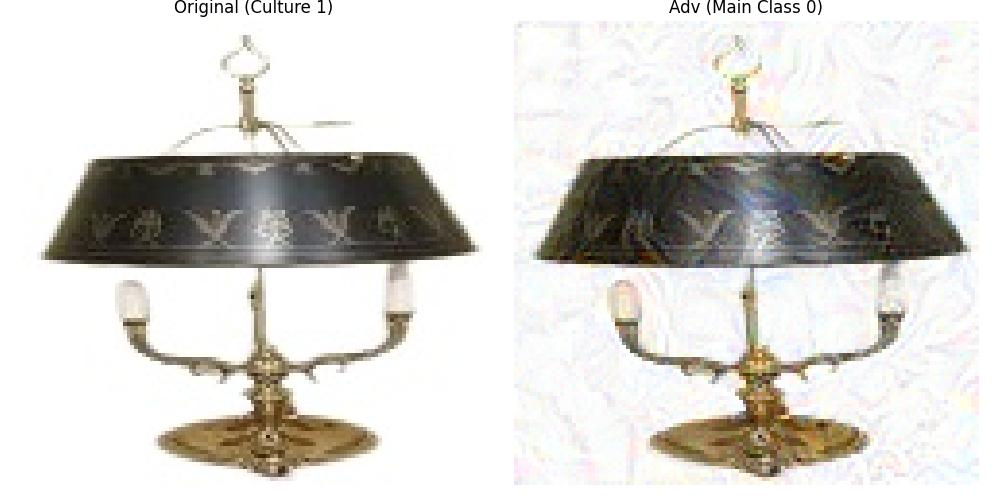
\includegraphics[width=\columnwidth]{adv_gen_figures/adv_02_majLC_NOCLSDIV0_source1.jpg}
\end{subfigure} \\
\begin{subfigure}[b]{0.6\columnwidth}
\centering
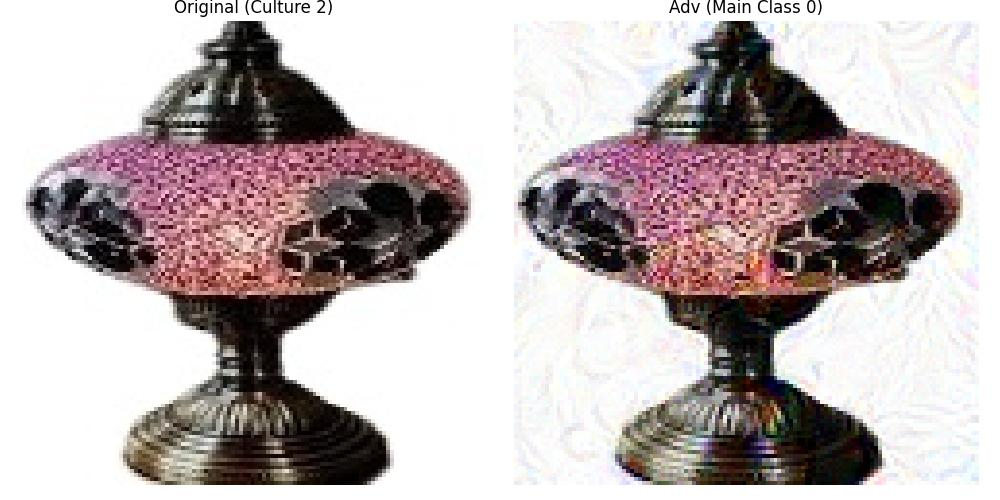
\includegraphics[width=\columnwidth]{adv_gen_figures/adv_02_majLC_NOCLSDIV0_source2.jpg}
\end{subfigure} 
\caption{Example of transformations applied on Chin., Fren. and Turk. images from LAMP dataset with lamps turned off using PGD and NOCLSDIV with Chin. as majority culture.}
\label{fig::adv02LC_NOCLSDIV0}
\end{figure}

\begin{figure}[H]
\centering
\begin{subfigure}[b]{0.6\columnwidth}
\centering
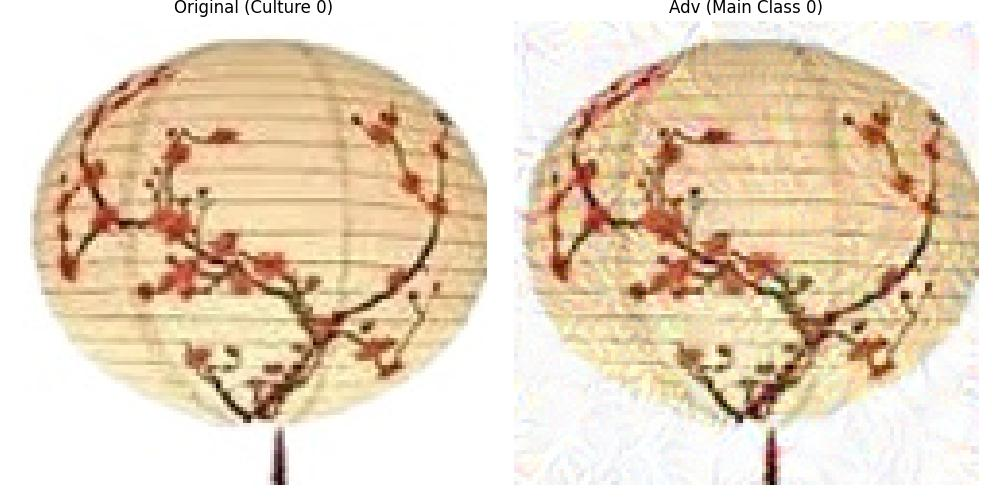
\includegraphics[width=\columnwidth]{adv_gen_figures/adv_02_majLF_NOCLSDIV0_source0.jpg}
\end{subfigure} \\
\begin{subfigure}[b]{0.6\columnwidth}
\centering
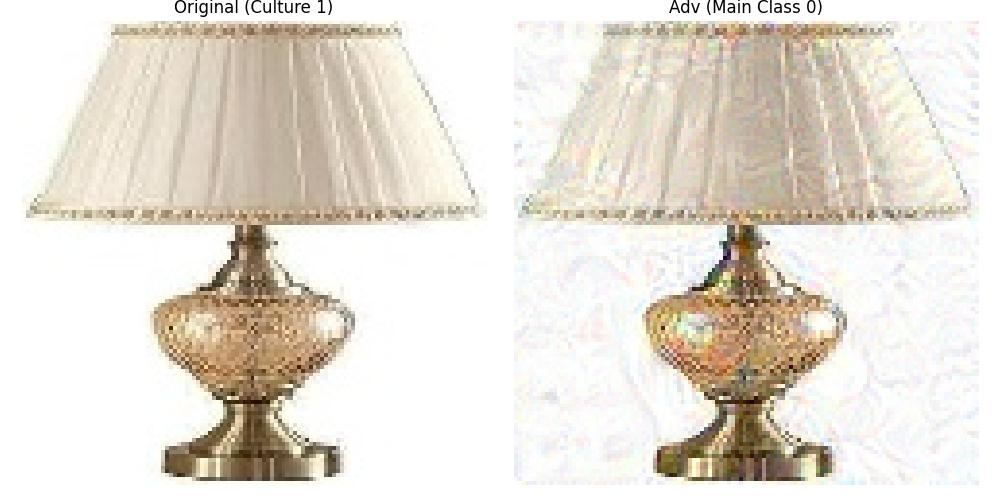
\includegraphics[width=\columnwidth]{adv_gen_figures/adv_02_majLF_NOCLSDIV0_source1.jpg}
\end{subfigure} \\
\begin{subfigure}[b]{0.6\columnwidth}
\centering
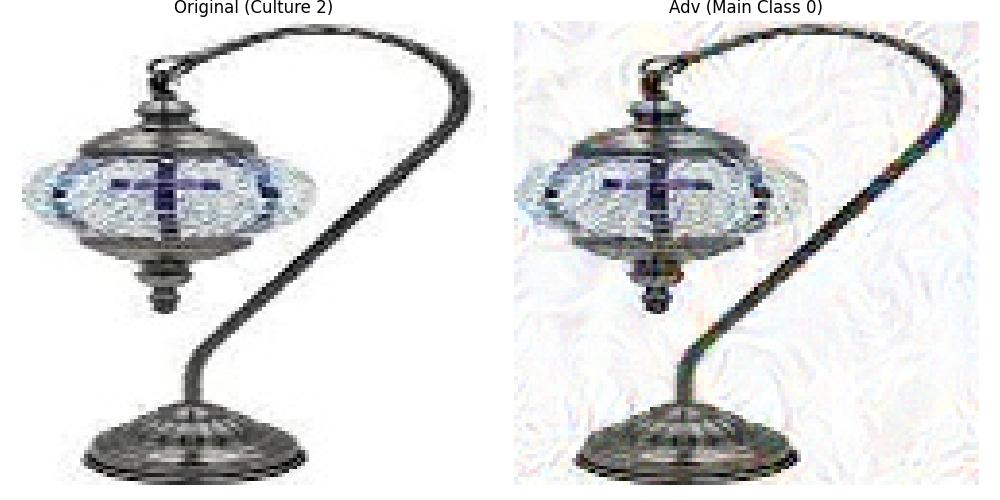
\includegraphics[width=\columnwidth]{adv_gen_figures/adv_02_majLF_NOCLSDIV0_source2.jpg}
\end{subfigure} 
\caption{Example of transformations applied on Chin., Fren. and Turk. images from LAMP dataset with lamps turned off using PGD and NOCLSDIV with Fren. as majority culture.}
\label{fig::adv02LF_NOCLSDIV0}
\end{figure}

\begin{figure}[H]
\centering
\begin{subfigure}[b]{0.6\columnwidth}
\centering
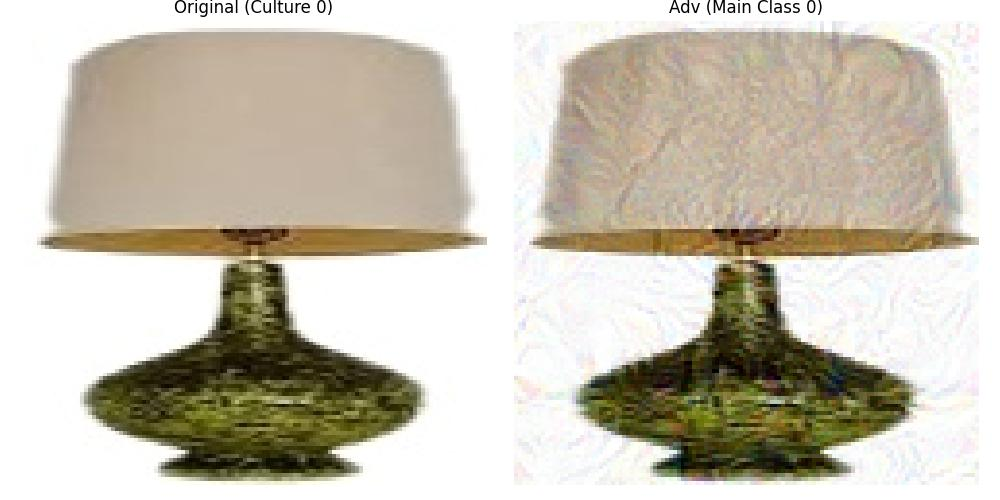
\includegraphics[width=\columnwidth]{adv_gen_figures/adv_02_majLT_NOCLSDIV0_source0.jpg}
\end{subfigure} \\
\begin{subfigure}[b]{0.6\columnwidth}
\centering
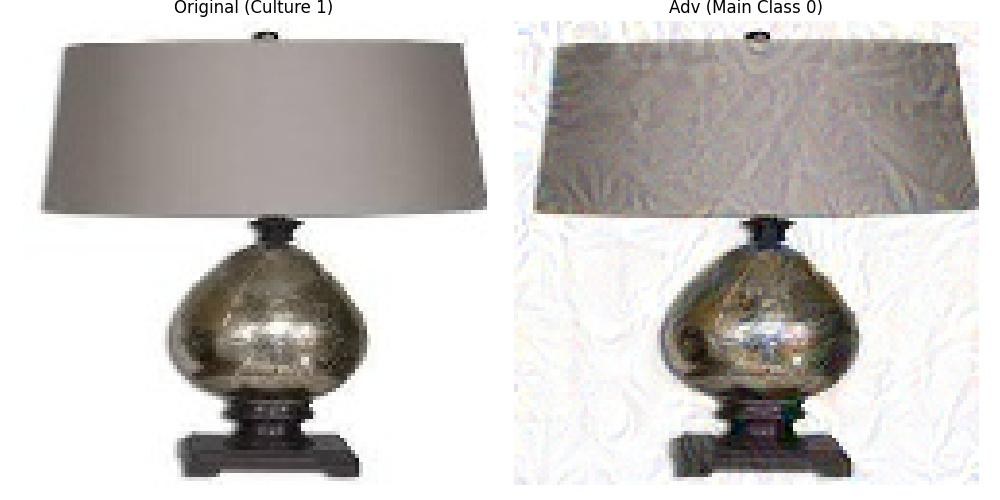
\includegraphics[width=\columnwidth]{adv_gen_figures/adv_02_majLT_NOCLSDIV0_source1.jpg}
\end{subfigure} \\
\begin{subfigure}[b]{0.6\columnwidth}
\centering
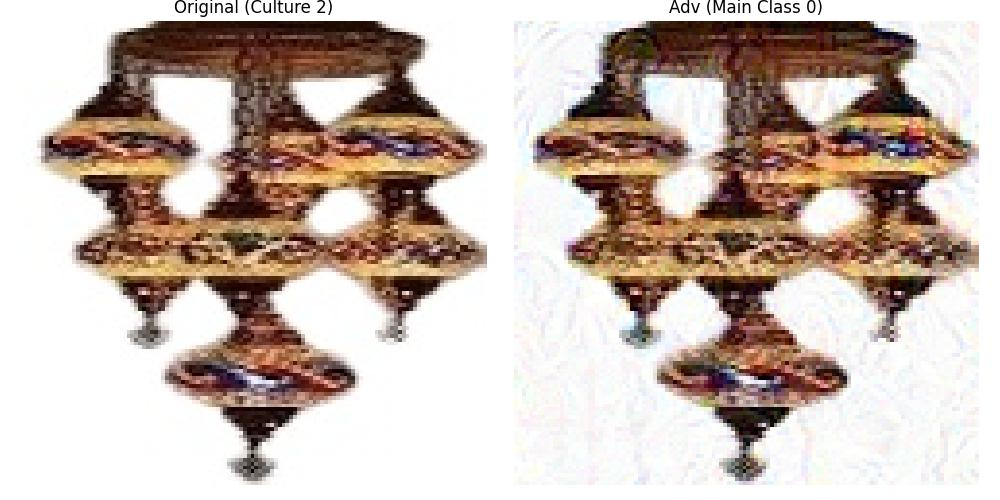
\includegraphics[width=\columnwidth]{adv_gen_figures/adv_02_majLT_NOCLSDIV0_source2.jpg}
\end{subfigure} 
\caption{Example of transformations applied on Chin., Fren. and Turk. images from LAMP dataset with lamps turned off using PGD and NOCLSDIV with Turk. as majority culture.}
\label{fig::adv02LT_NOCLSDIV0}
\end{figure}

% NOCLSDIV 1
\begin{figure}[H]
\centering
\begin{subfigure}[b]{0.6\columnwidth}
\centering
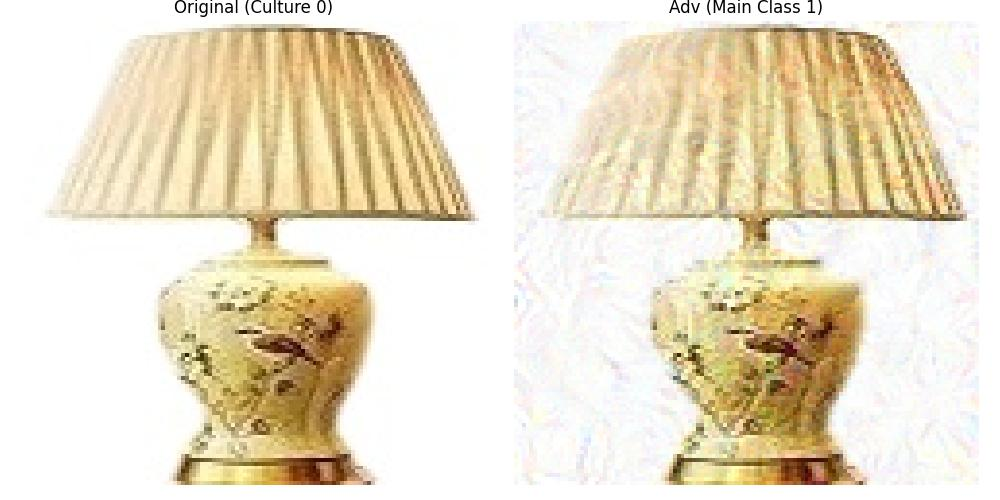
\includegraphics[width=\columnwidth]{adv_gen_figures/adv_02_majLC_NOCLSDIV1_source0.jpg}
\end{subfigure} \\
\begin{subfigure}[b]{0.6\columnwidth}
\centering
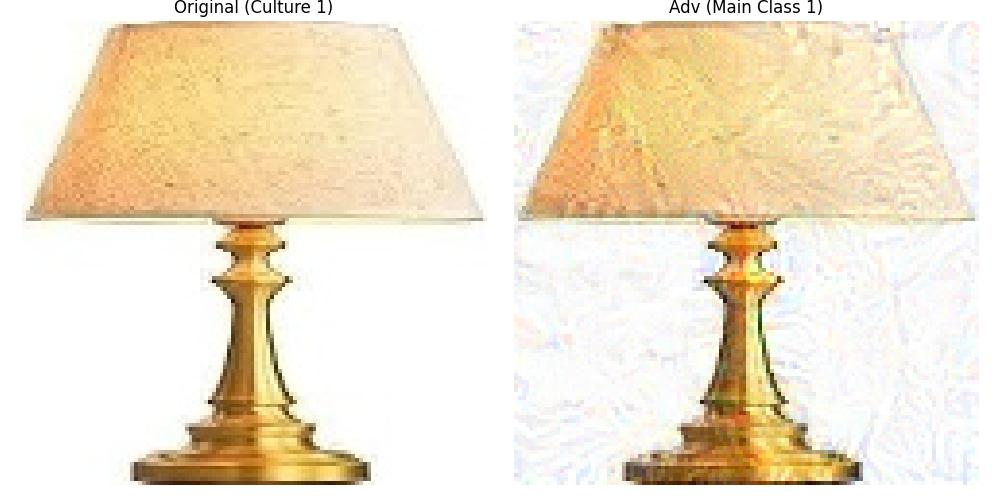
\includegraphics[width=\columnwidth]{adv_gen_figures/adv_02_majLC_NOCLSDIV1_source1.jpg}
\end{subfigure} \\
\begin{subfigure}[b]{0.6\columnwidth}
\centering
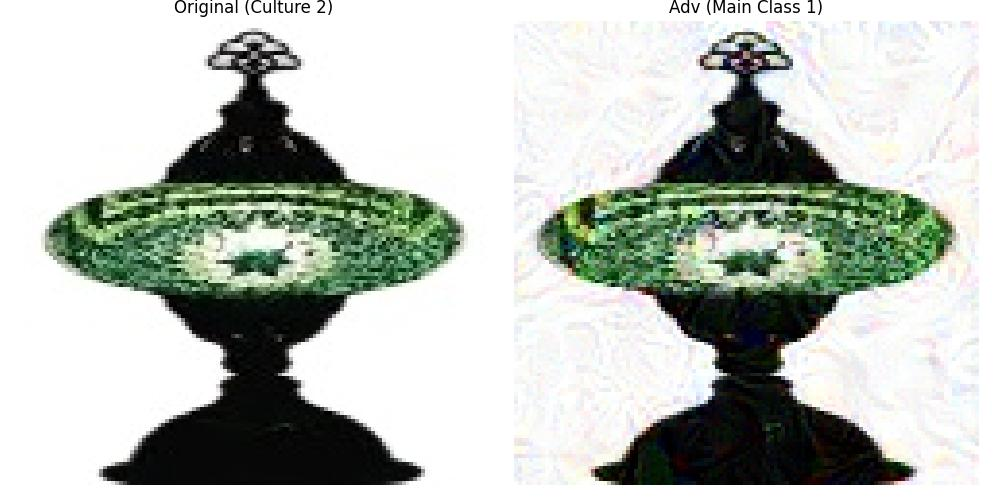
\includegraphics[width=\columnwidth]{adv_gen_figures/adv_02_majLC_NOCLSDIV1_source2.jpg}
\end{subfigure} 
\caption{Example of transformations applied on Chin., Fren. and Turk. images from LAMP dataset with lamps turned on using PGD and NOCLSDIV with Chin. as majority culture.}
\label{fig::adv02LC_NOCLSDIV1}
\end{figure}

\begin{figure}[H]
\centering
\begin{subfigure}[b]{0.6\columnwidth}
\centering
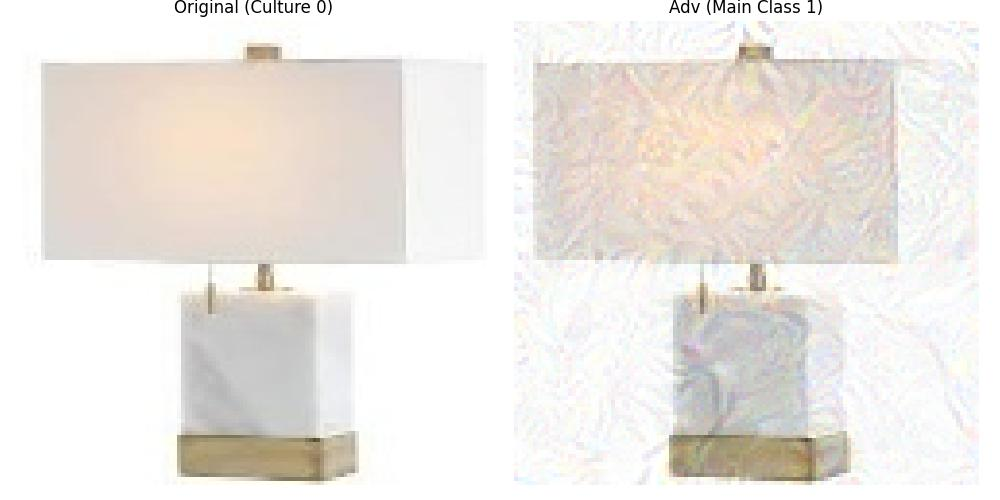
\includegraphics[width=\columnwidth]{adv_gen_figures/adv_02_majLF_NOCLSDIV1_source0.jpg}
\end{subfigure} \\
\begin{subfigure}[b]{0.6\columnwidth}
\centering
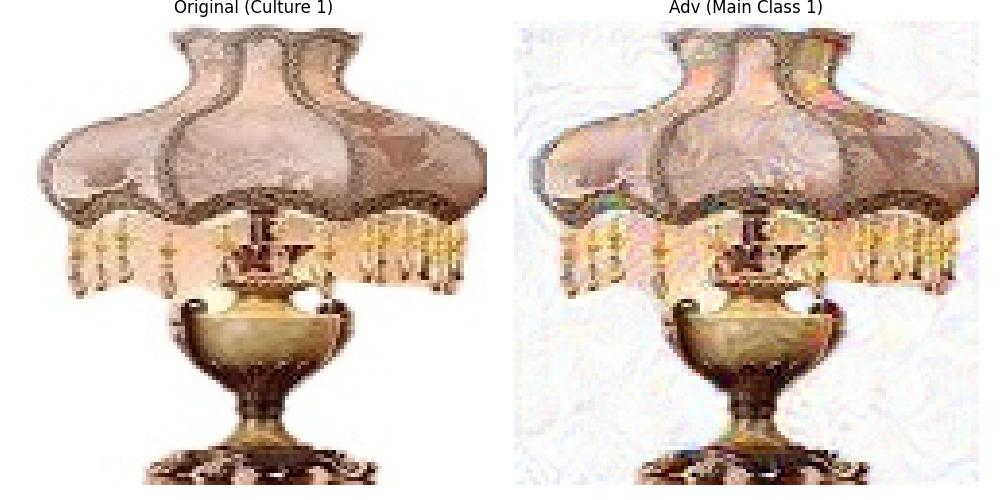
\includegraphics[width=\columnwidth]{adv_gen_figures/adv_02_majLF_NOCLSDIV1_source1.jpg}
\end{subfigure} \\
\begin{subfigure}[b]{0.6\columnwidth}
\centering
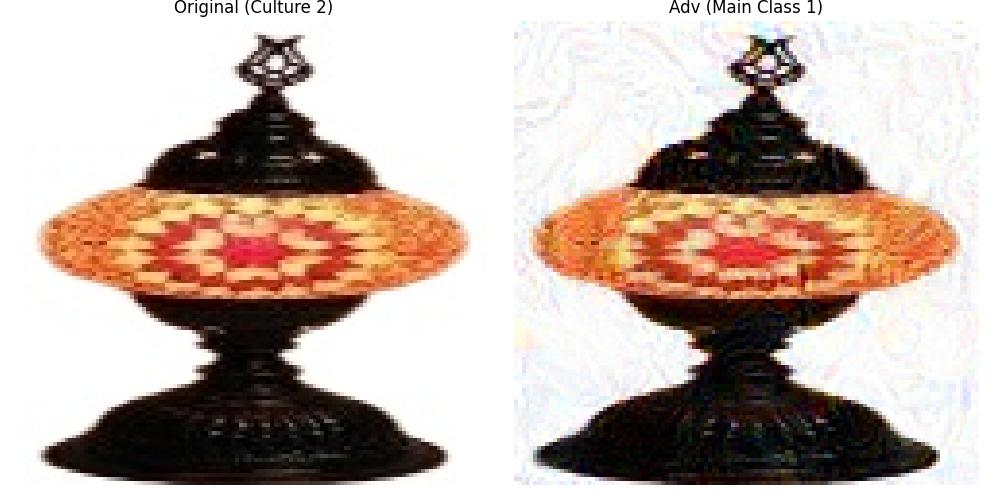
\includegraphics[width=\columnwidth]{adv_gen_figures/adv_02_majLF_NOCLSDIV1_source2.jpg}
\end{subfigure} 
\caption{Example of transformations applied on Chin., Fren. and Turk. images from LAMP dataset with lamps turned on using PGD and NOCLSDIV with Fren. as majority culture.}
\label{fig::adv02LF_NOCLSDIV1}
\end{figure}

\begin{figure}[H]
\centering
\begin{subfigure}[b]{0.6\columnwidth}
\centering
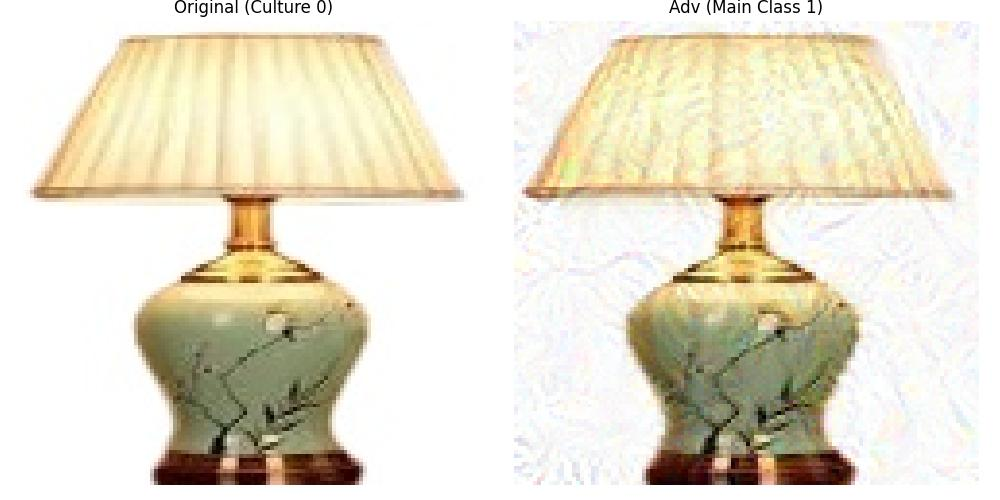
\includegraphics[width=\columnwidth]{adv_gen_figures/adv_02_majLT_NOCLSDIV1_source0.jpg}
\end{subfigure} \\
\begin{subfigure}[b]{0.6\columnwidth}
\centering
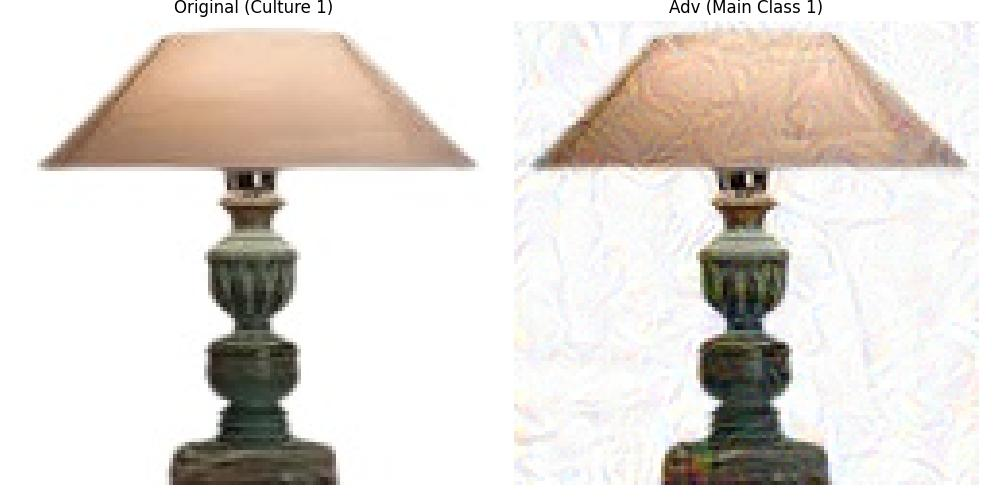
\includegraphics[width=\columnwidth]{adv_gen_figures/adv_02_majLT_NOCLSDIV1_source1.jpg}
\end{subfigure} \\
\begin{subfigure}[b]{0.6\columnwidth}
\centering
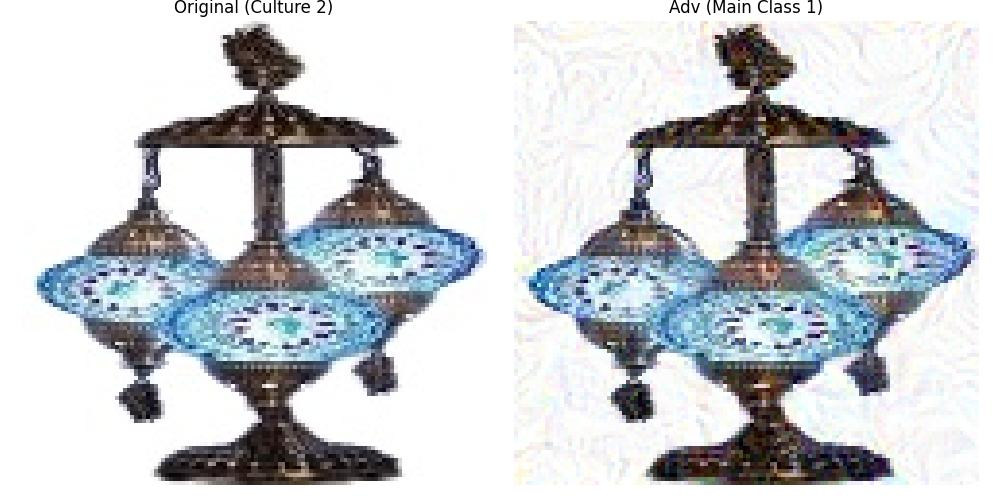
\includegraphics[width=\columnwidth]{adv_gen_figures/adv_02_majLT_NOCLSDIV1_source2.jpg}
\end{subfigure} 
\caption{Example of transformations applied on Chin., Fren. and Turk. images from LAMP dataset with lamps turned on using PGD and NOCLSDIV with Turk. as majority culture.}
\label{fig::adv02LT_NOCLSDIV1}
\end{figure}

% CARPET
Tables~\ref{fig::adv02CI_CLSDIV0}, \ref{fig::adv02CI_CLSDIV1}, \ref{fig::adv02CI_NOCLSDIV0}, \ref{fig::adv02CI_NOCLSDIV1}, \ref{fig::adv02CJ_CLSDIV0}, \ref{fig::adv02CJ_CLSDIV1}, \ref{fig::adv02CJ_NOCLSDIV0}, \ref{fig::adv02CJ_NOCLSDIV1},
\ref{fig::adv02CS_CLSDIV0}, \ref{fig::adv02CS_CLSDIV1}, \ref{fig::adv02CS_NOCLSDIV0}, \ref{fig::adv02CS_NOCLSDIV1} show examples of transformations applied on Ind., Jap., and Scan. images from CARPET dataset with lamps turned off using PGD, and CLSDIV or NOCLSDIV with Ind., Jap., and Scan. as majority cultures with $p_u=20\%$.
\begin{figure}[H]
\centering
\begin{subfigure}[b]{0.6\columnwidth}
\centering
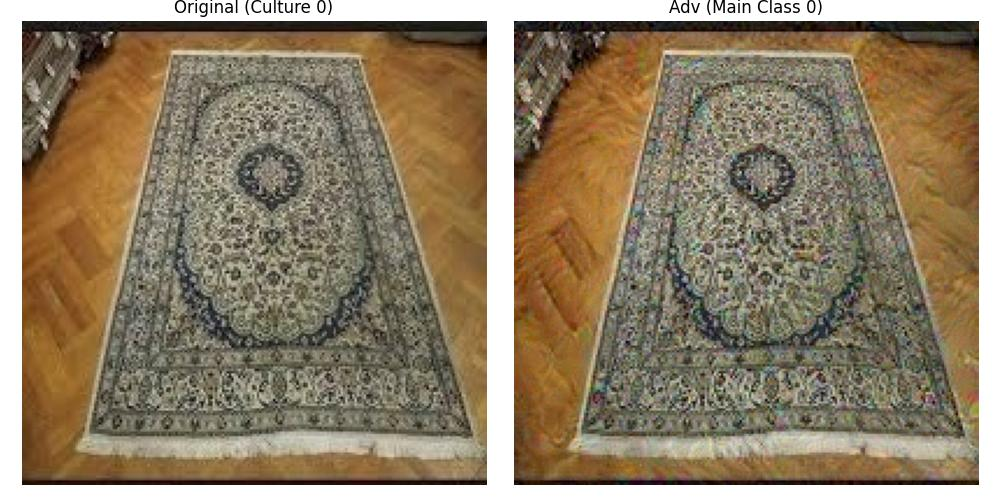
\includegraphics[width=\columnwidth]{adv_gen_figures/adv_02_majCI_CLSDIV0_source0.jpg}
\end{subfigure} \\
\begin{subfigure}[b]{0.6\columnwidth}
\centering
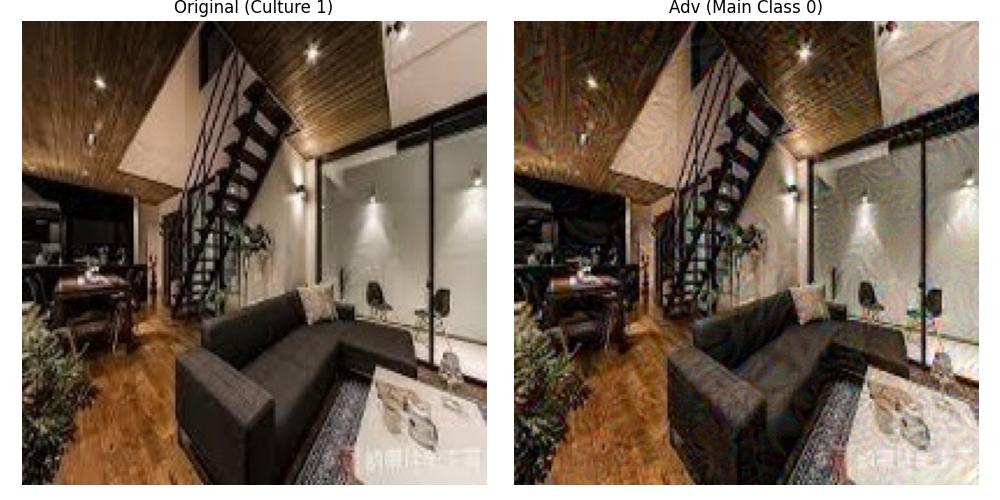
\includegraphics[width=\columnwidth]{adv_gen_figures/adv_02_majCI_CLSDIV0_source1.jpg}
\end{subfigure} \\
\begin{subfigure}[b]{0.6\columnwidth}
\centering
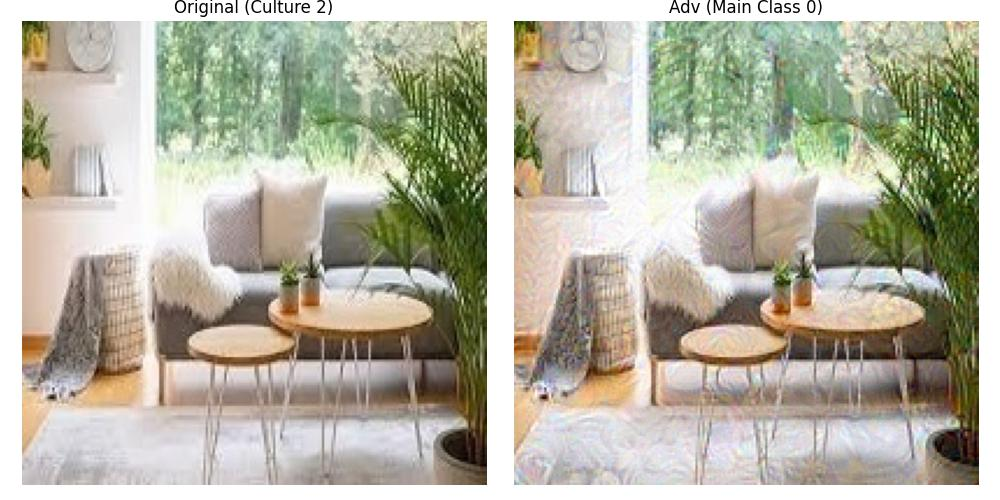
\includegraphics[width=\columnwidth]{adv_gen_figures/adv_02_majCI_CLSDIV0_source2.jpg}
\end{subfigure} 
\caption{Example of transformations applied on Ind. Jap. and Scan. dataset with with carpets using PGD and CLSDIV with Ind. as majority culture.}
\label{fig::adv02CI_CLSDIV0}
\end{figure}

\begin{figure}[H]
\centering
\begin{subfigure}[b]{0.6\columnwidth}
\centering
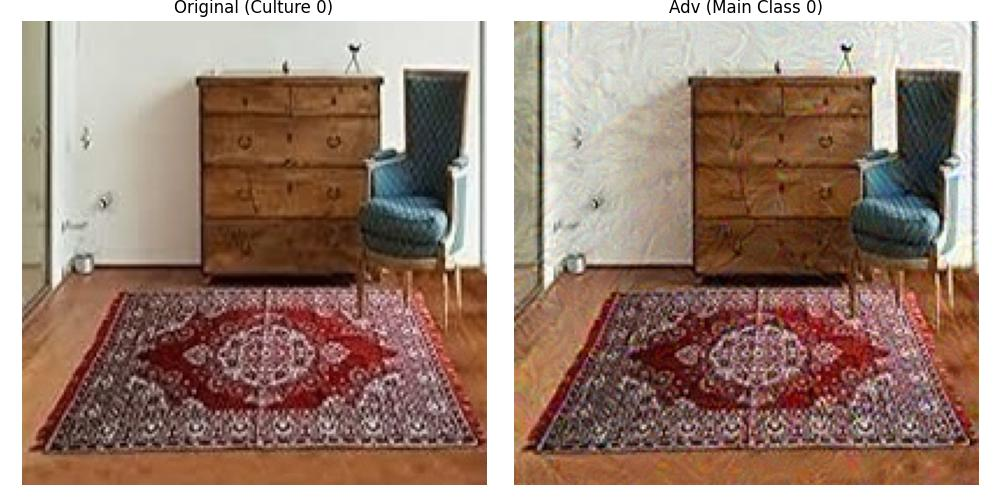
\includegraphics[width=\columnwidth]{adv_gen_figures/adv_02_majCJ_CLSDIV0_source0.jpg}

\end{subfigure} \\
\begin{subfigure}[b]{0.6\columnwidth}
\centering
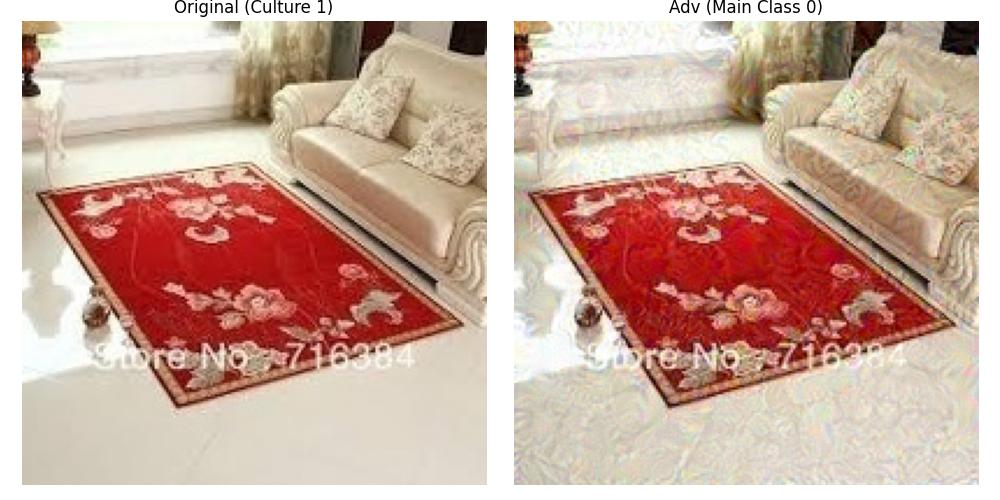
\includegraphics[width=\columnwidth]{adv_gen_figures/adv_02_majCJ_CLSDIV0_source1.jpg}
\end{subfigure} \\
\begin{subfigure}[b]{0.6\columnwidth}
\centering
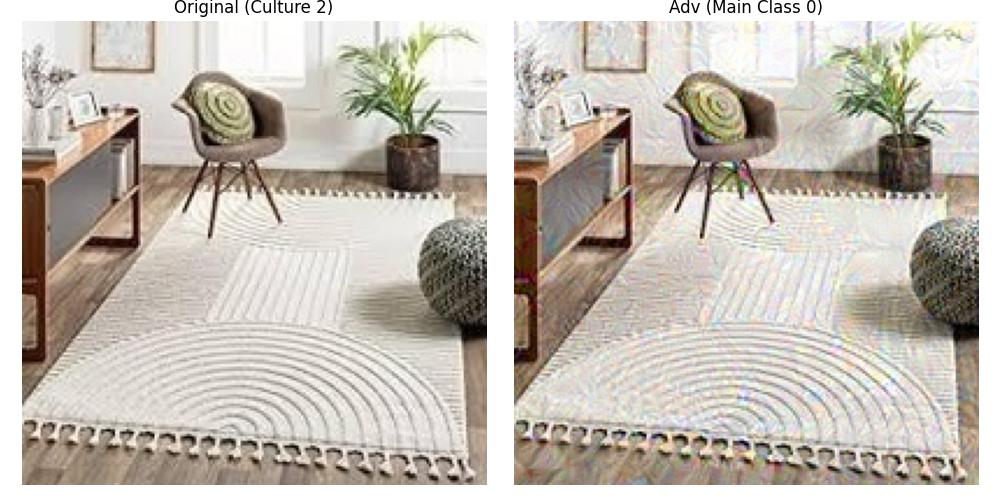
\includegraphics[width=\columnwidth]{adv_gen_figures/adv_02_majCJ_CLSDIV0_source2.jpg}
\end{subfigure} 
\caption{Example of transformations applied on Ind. Jap. and Scan. dataset with with carpets using PGD and CLSDIV with Jap. as majority culture.}
\label{fig::adv02CJ_CLSDIV0}
\end{figure}

\begin{figure}[H]
\centering
\begin{subfigure}[b]{0.6\columnwidth}
\centering
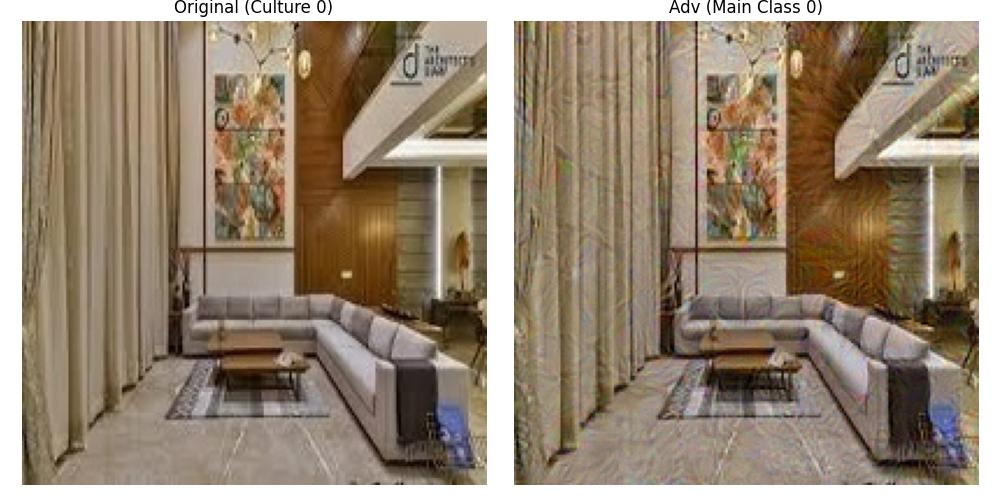
\includegraphics[width=\columnwidth]{adv_gen_figures/adv_02_majCS_CLSDIV0_source0.jpg}
\end{subfigure} \\
\begin{subfigure}[b]{0.6\columnwidth}
\centering
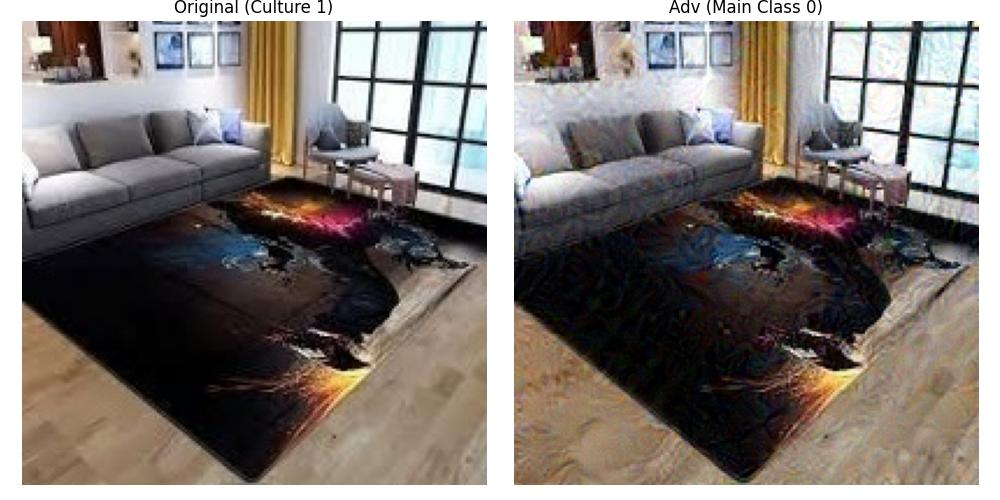
\includegraphics[width=\columnwidth]{adv_gen_figures/adv_02_majCS_CLSDIV0_source1.jpg}
\end{subfigure} \\
\begin{subfigure}[b]{0.6\columnwidth}
\centering
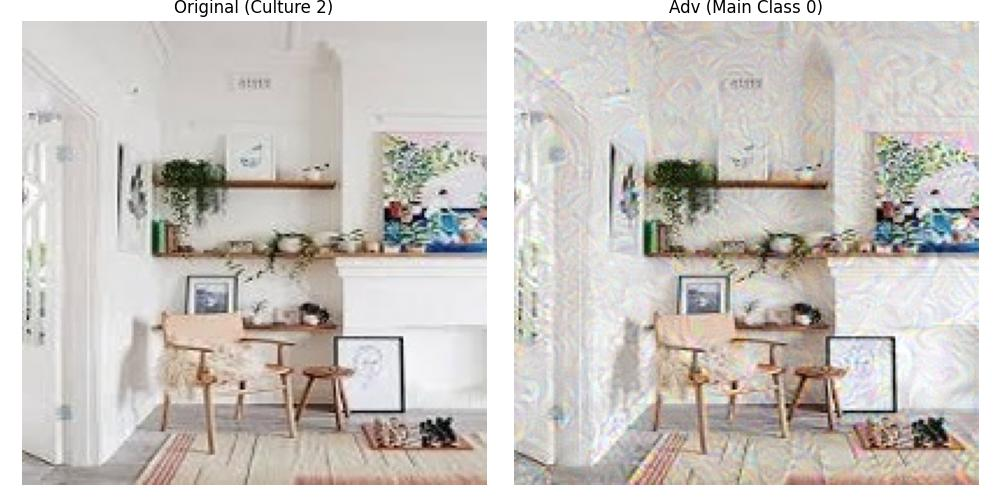
\includegraphics[width=\columnwidth]{adv_gen_figures/adv_02_majCS_CLSDIV0_source2.jpg}
\end{subfigure} 
\caption{Example of transformations applied on Ind. Jap. and Scan. dataset with with carpets using PGD and CLSDIV with Scan. as majority culture.}
\label{fig::adv02CS_CLSDIV0}
\end{figure}

%CLSDIV 1
\begin{figure}[H]
\centering
\begin{subfigure}[b]{0.6\columnwidth}
\centering
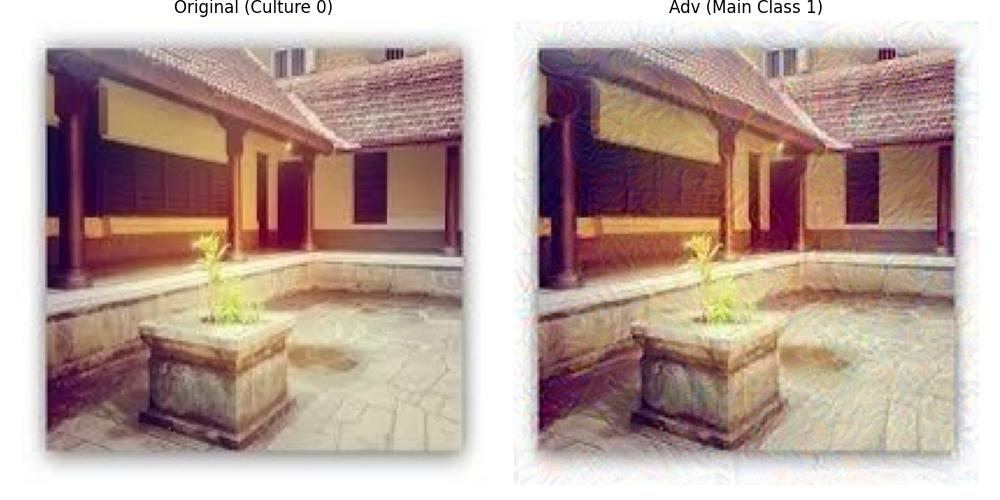
\includegraphics[width=\columnwidth]{adv_gen_figures/adv_02_majCI_CLSDIV1_source0.jpg}
\end{subfigure} \\
\begin{subfigure}[b]{0.6\columnwidth}
\centering
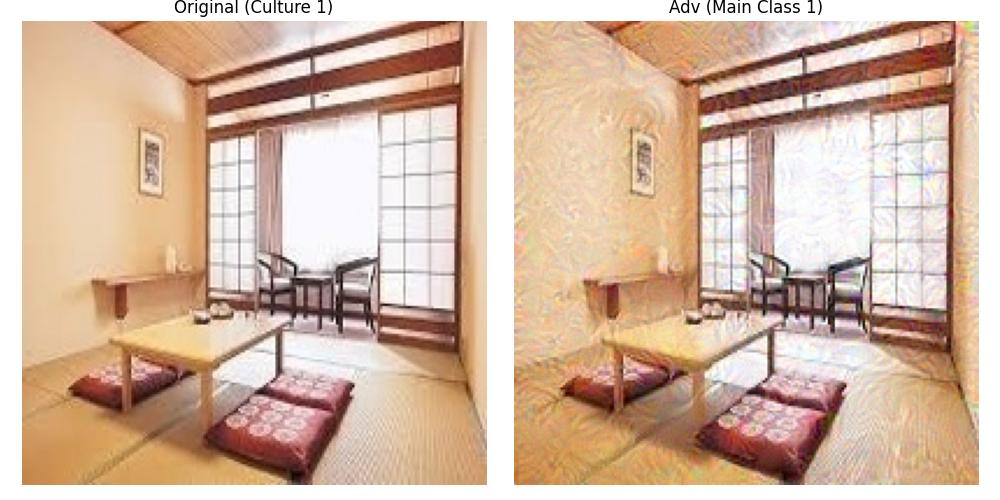
\includegraphics[width=\columnwidth]{adv_gen_figures/adv_02_majCI_CLSDIV1_source1.jpg}
\end{subfigure} \\
\begin{subfigure}[b]{0.6\columnwidth}
\centering
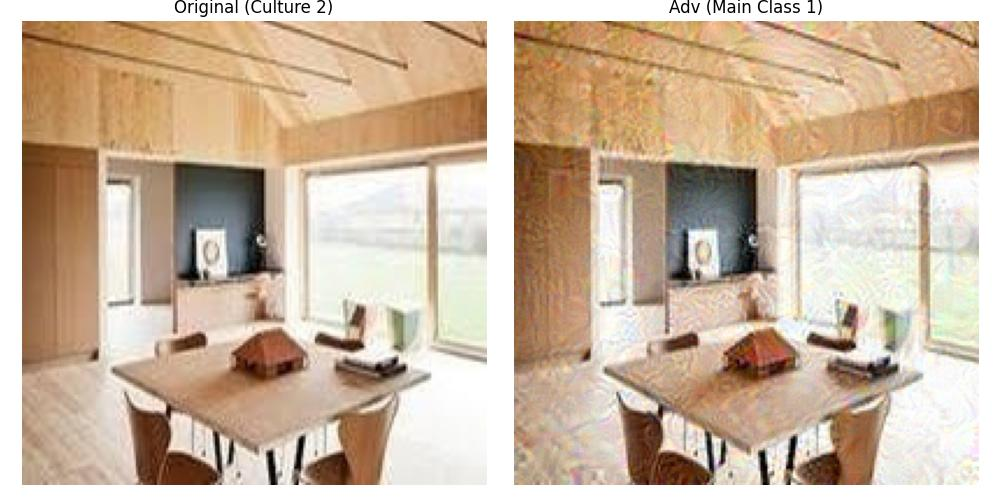
\includegraphics[width=\columnwidth]{adv_gen_figures/adv_02_majCI_CLSDIV1_source2.jpg}
\end{subfigure} 
\caption{Example of transformations applied on Ind. Jap. and Scan. dataset without carpets using PGD and CLSDIV with Ind. as majority culture.}
\label{fig::adv02CI_CLSDIV1}
\end{figure}

\begin{figure}[H]
\centering
\begin{subfigure}[b]{0.6\columnwidth}
\centering
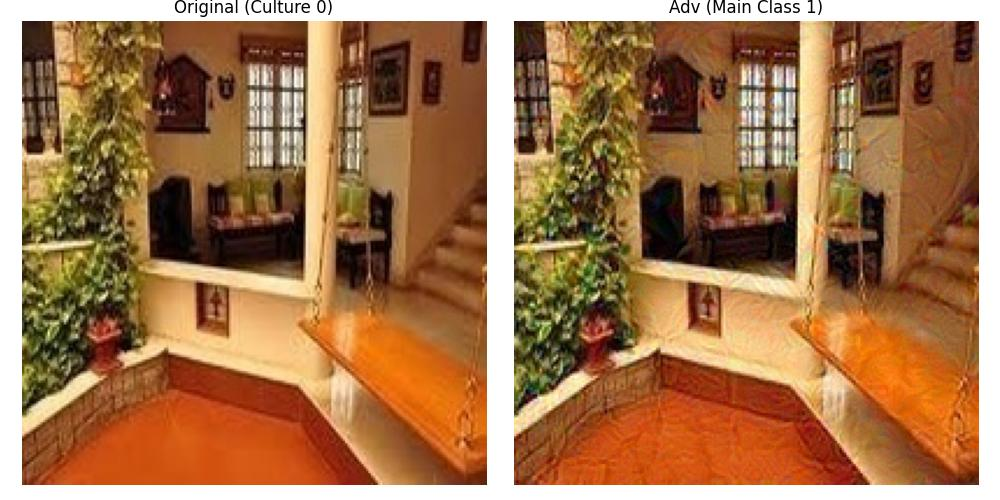
\includegraphics[width=\columnwidth]{adv_gen_figures/adv_02_majCJ_CLSDIV1_source0.jpg}
\end{subfigure} \\
\begin{subfigure}[b]{0.6\columnwidth}
\centering
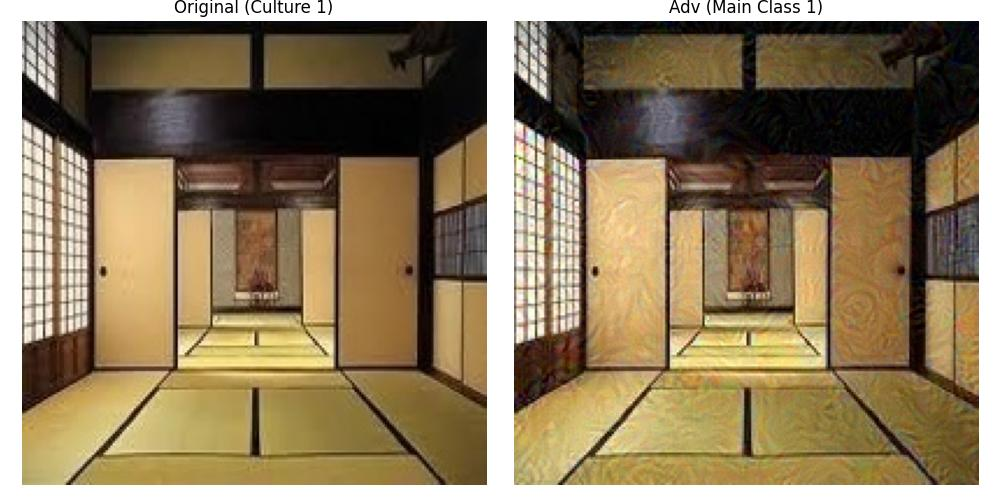
\includegraphics[width=\columnwidth]{adv_gen_figures/adv_02_majCJ_CLSDIV1_source1.jpg}
\end{subfigure} \\
\begin{subfigure}[b]{0.6\columnwidth}
\centering
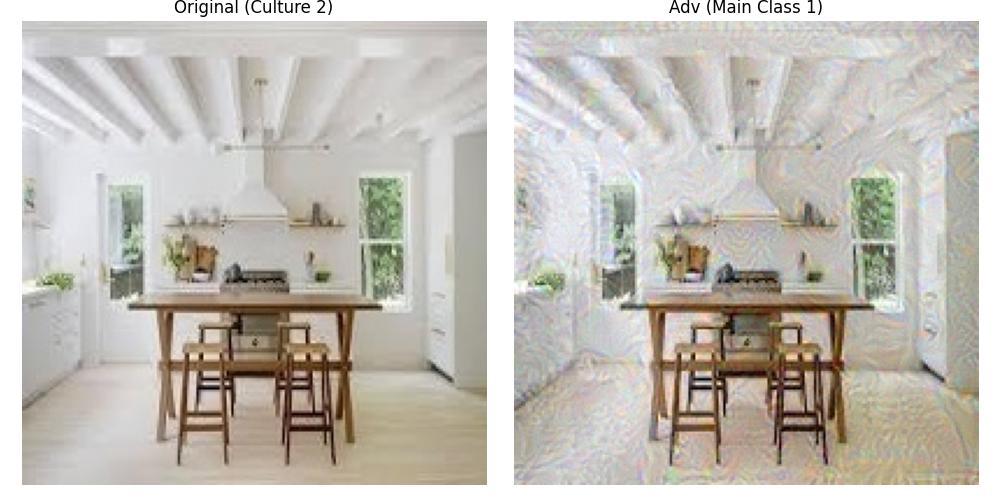
\includegraphics[width=\columnwidth]{adv_gen_figures/adv_02_majCJ_CLSDIV1_source2.jpg}
\end{subfigure} 
\caption{Example of transformations applied on Ind. Jap. and Scan. dataset without carpets using PGD and CLSDIV with Jap. as majority culture.}
\label{fig::adv02CJ_CLSDIV1}
\end{figure}

\begin{figure}[H]
\centering
\begin{subfigure}[b]{0.6\columnwidth}
\centering
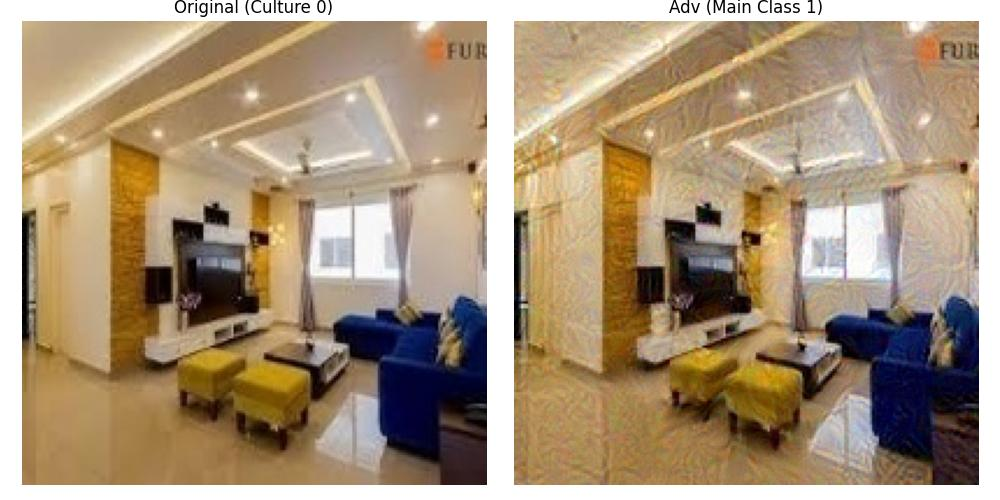
\includegraphics[width=\columnwidth]{adv_gen_figures/adv_02_majCS_CLSDIV1_source0.jpg}
\end{subfigure} \\
\begin{subfigure}[b]{0.6\columnwidth}
\centering
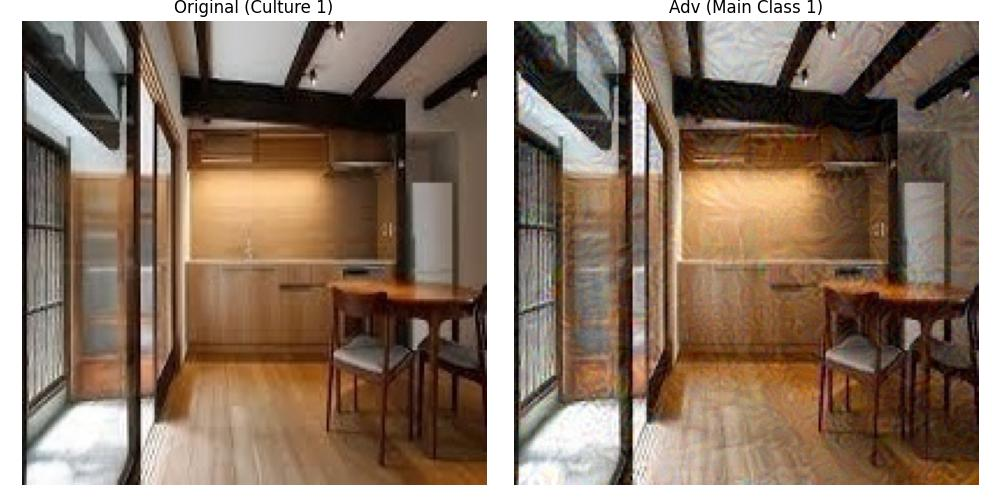
\includegraphics[width=\columnwidth]{adv_gen_figures/adv_02_majCS_CLSDIV1_source1.jpg}
\end{subfigure} \\
\begin{subfigure}[b]{0.6\columnwidth}
\centering
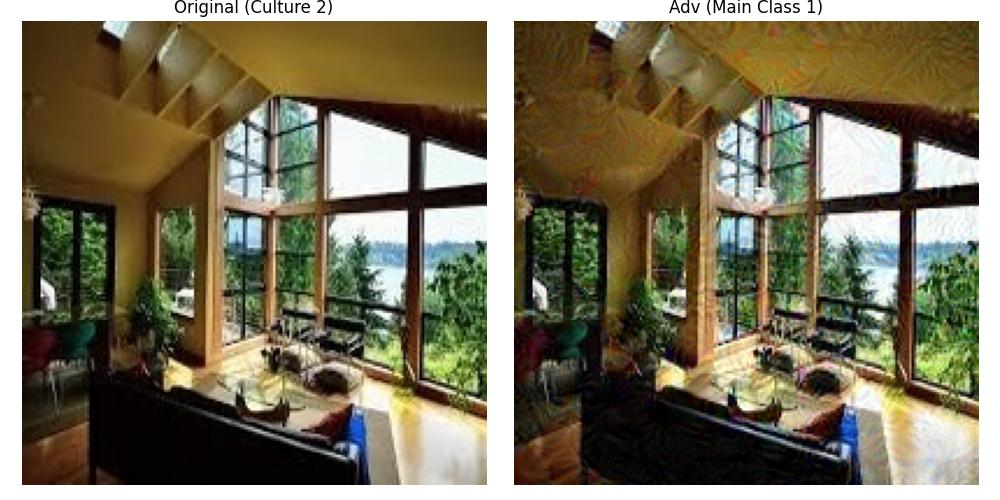
\includegraphics[width=\columnwidth]{adv_gen_figures/adv_02_majCS_CLSDIV1_source2.jpg}
\end{subfigure} 
\caption{Example of transformations applied on Ind. Jap. and Scan. dataset without carpets using PGD and CLSDIV with Scan. as majority culture.}
\label{fig::adv02CS_CLSDIV1}
\end{figure}

% NOCLSDIV 0
\begin{figure}[H]
\centering
\begin{subfigure}[b]{0.6\columnwidth}
\centering
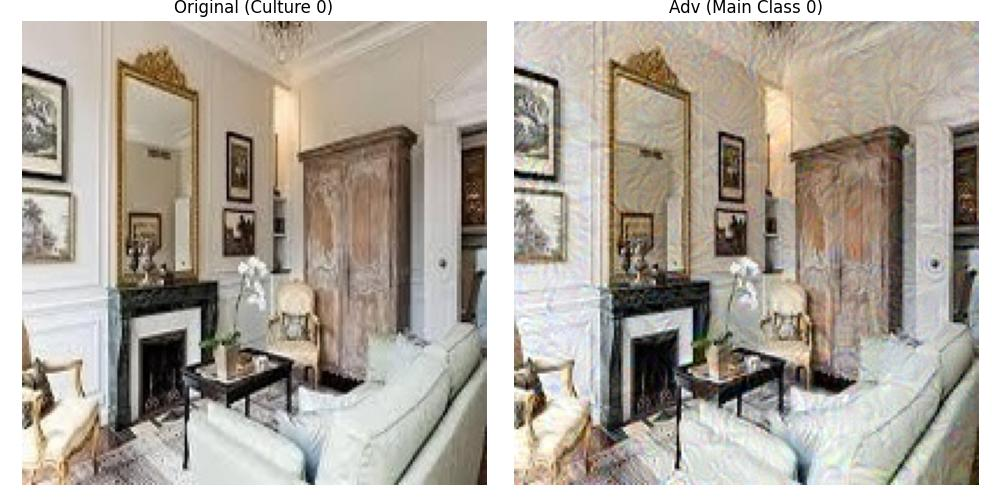
\includegraphics[width=\columnwidth]{adv_gen_figures/adv_02_majCI_NOCLSDIV0_source0.jpg}
\end{subfigure} \\
\begin{subfigure}[b]{0.6\columnwidth}
\centering
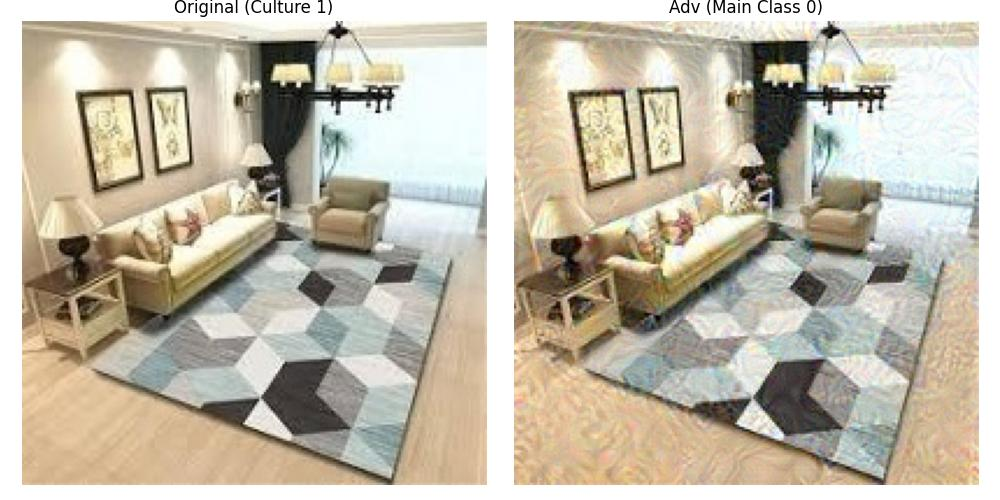
\includegraphics[width=\columnwidth]{adv_gen_figures/adv_02_majCI_NOCLSDIV0_source1.jpg}
\end{subfigure} \\
\begin{subfigure}[b]{0.6\columnwidth}
\centering
\includegraphics[width=\columnwidth]{adv_gen_figures/adv_02_majCI_NOCLSDIV0_source2.jpg}
\end{subfigure} 
\caption{Example of transformations applied on Ind. Jap. and Scan. dataset with with carpets using PGD and NOCLSDIV with Ind. as majority culture.}
\label{fig::adv02CI_NOCLSDIV0}
\end{figure}

\begin{figure}[H]
\centering
\begin{subfigure}[b]{0.6\columnwidth}
\centering
\includegraphics[width=\columnwidth]{adv_gen_figures/adv_02_majCJ_NOCLSDIV0_source0.jpg}
\end{subfigure} \\
\begin{subfigure}[b]{0.6\columnwidth}
\centering
\includegraphics[width=\columnwidth]{adv_gen_figures/adv_02_majCJ_NOCLSDIV0_source1.jpg}
\end{subfigure} \\
\begin{subfigure}[b]{0.6\columnwidth}
\centering
\includegraphics[width=\columnwidth]{adv_gen_figures/adv_02_majCJ_NOCLSDIV0_source2.jpg}
\end{subfigure} 
\caption{Example of transformations applied on Ind. Jap. and Scan. dataset with with carpets using PGD and NOCLSDIV with Jap. as majority culture.}
\label{fig::adv02CJ_NOCLSDIV0}
\end{figure}

\begin{figure}[H]
\centering
\begin{subfigure}[b]{0.6\columnwidth}
\centering
\includegraphics[width=\columnwidth]{adv_gen_figures/adv_02_majCS_NOCLSDIV0_source0.jpg}
\end{subfigure} \\
\begin{subfigure}[b]{0.6\columnwidth}
\centering
\includegraphics[width=\columnwidth]{adv_gen_figures/adv_02_majCS_NOCLSDIV0_source1.jpg}
\end{subfigure} \\
\begin{subfigure}[b]{0.6\columnwidth}
\centering
\includegraphics[width=\columnwidth]{adv_gen_figures/adv_02_majCS_NOCLSDIV0_source2.jpg}
\end{subfigure} 
\caption{Example of transformations applied on Ind. Jap. and Scan. dataset with with carpets using PGD and NOCLSDIV with Scan. as majority culture.}
\label{fig::adv02CS_NOCLSDIV0}
\end{figure}

% NOCLSDIV 1
\begin{figure}[H]
\centering
\begin{subfigure}[b]{0.6\columnwidth}
\centering
\includegraphics[width=\columnwidth]{adv_gen_figures/adv_02_majCI_NOCLSDIV1_source0.jpg}
\end{subfigure} \\
\begin{subfigure}[b]{0.6\columnwidth}
\centering
\includegraphics[width=\columnwidth]{adv_gen_figures/adv_02_majCI_NOCLSDIV1_source1.jpg}
\end{subfigure} \\
\begin{subfigure}[b]{0.6\columnwidth}
\centering
\includegraphics[width=\columnwidth]{adv_gen_figures/adv_02_majCI_NOCLSDIV1_source2.jpg}
\end{subfigure} 
\caption{Example of transformations applied on Ind. Jap. and Scan. dataset without carpets using PGD and NOCLSDIV with Ind. as majority culture.}
\label{fig::adv02CI_NOCLSDIV1}
\end{figure}

\begin{figure}[H]
\centering
\begin{subfigure}[b]{0.6\columnwidth}
\centering
\includegraphics[width=\columnwidth]{adv_gen_figures/adv_02_majCJ_NOCLSDIV1_source0.jpg}
\end{subfigure} \\
\begin{subfigure}[b]{0.6\columnwidth}
\centering
\includegraphics[width=\columnwidth]{adv_gen_figures/adv_02_majCJ_NOCLSDIV1_source1.jpg}
\end{subfigure} \\
\begin{subfigure}[b]{0.6\columnwidth}
\centering
\includegraphics[width=\columnwidth]{adv_gen_figures/adv_02_majCJ_NOCLSDIV1_source2.jpg}
\end{subfigure} 
\caption{Example of transformations applied on Ind. Jap. and Scan. dataset without carpets using PGD and NOCLSDIV with Jap. as majority culture.}
\label{fig::adv02CJ_NOCLSDIV1}
\end{figure}

\begin{figure}[H]
\centering
\begin{subfigure}[b]{0.6\columnwidth}
\centering
\includegraphics[width=\columnwidth]{adv_gen_figures/adv_02_majCS_NOCLSDIV1_source0.jpg}
\end{subfigure} \\
\begin{subfigure}[b]{0.6\columnwidth}
\centering
\includegraphics[width=\columnwidth]{adv_gen_figures/adv_02_majCS_NOCLSDIV1_source1.jpg}
\end{subfigure} \\
\begin{subfigure}[b]{0.6\columnwidth}
\centering
\includegraphics[width=\columnwidth]{adv_gen_figures/adv_02_majCS_NOCLSDIV1_source2.jpg}
\end{subfigure} 
\caption{Example of transformations applied on Ind. Jap. and Scan. dataset without carpets using PGD and NOCLSDIV with Scan. as majority culture.}
\label{fig::adv02CS_NOCLSDIV1}
\end{figure}

\subsection{Diffusion Generated Images}

%
%%%%%%%%%%%% DM %%%%%%%%%%%%%
%
Tables~\ref{ch4:fig:diff_gen_LAMP_DM_LC}, \ref{ch4:fig:diff_gen_LAMP_DM_LF}, \ref{ch4:fig:diff_gen_LAMP_DM_LT}, \ref{ch4:fig:diff_gen_LAMP_DMMIN_LC}, \ref{ch4:fig:diff_gen_LAMP_DMMIN_LF}, \ref{ch4:fig:diff_gen_LAMP_DMMIN_LT}, \ref{ch4:fig:diff_gen_LAMP_DM_PARBS_LC}, \ref{ch4:fig:diff_gen_LAMP_DM_PARBS_LF}, \ref{ch4:fig:diff_gen_LAMP_DM_PARBS_LT}, \ref{ch4:fig:diff_gen_LAMP_DMMIN_PARBS_LC}, \ref{ch4:fig:diff_gen_LAMP_DMMIN_PARBS_LF}, \ref{ch4:fig:diff_gen_LAMP_DMMIN_PARBS_LT} show examples of images generated using DM, DMMIN and PARBS  on LAMP dataset with Chin., Fre. and Turk. as majority culture.

\begin{figure}
    \centering
    \begin{subfigure}[b]{0.7\columnwidth} 
        \includegraphics[width=\columnwidth]{diff_gen_figures/Lamps0_0_imb=0.png}
        \caption{Data generated using Chin. culture as majority culture and lamps turned off.}
    \end{subfigure} \\
    \begin{subfigure}[b]{0.7\columnwidth} 
        \includegraphics[width=\columnwidth]{diff_gen_figures/Lamps0_1_imb=0.png}
        \caption{Data generated using Chin. culture as majority culture and lamps turned on.}
    \end{subfigure}
\caption{Examples of images generated using DM on LAMP dataset with Chin. as majority culture.}
\label{ch4:fig:diff_gen_LAMP_DM_LC}
\end{figure}
\begin{figure}
    \centering
    \begin{subfigure}[b]{0.7\columnwidth}  
        \includegraphics[width=\columnwidth]{diff_gen_figures/Lamps1_0_imb=0.png}
        \caption{Data generated using Fren. culture as majority culture and lamps turned off.}
    \end{subfigure} \\
    \begin{subfigure}[b]{0.7\columnwidth} 
        \includegraphics[width=\columnwidth]{diff_gen_figures/Lamps1_0_imb=0.png}
        \caption{Data generated using Fren. culture as majority culture and lamps turned on.}
    \end{subfigure}
\caption{Examples of images generated using DM on LAMP dataset with Fren. as majority culture.}
\label{ch4:fig:diff_gen_LAMP_DM_LF}
\end{figure}
\begin{figure}
    \centering
    \begin{subfigure}[b]{0.7\columnwidth} 
        \includegraphics[width=\columnwidth]{diff_gen_figures/Lamps2_0_imb=0.png}
        \caption{Data generated using Turk. culture as majority culture and lamps turned off.}
    \end{subfigure} \\
    \begin{subfigure}[b]{0.7\columnwidth}  
        \includegraphics[width=\columnwidth]{diff_gen_figures/Lamps2_0_imb=0.png}
        \caption{Data generated using Turk. culture as majority culture and lamps turned on.}
    \end{subfigure} 
    \caption{Examples of images generated using DM on LAMP dataset with Turk. as majority culture.}
    \label{ch4:fig:diff_gen_LAMP_DM_LT}
\end{figure}
%
%%%%%%%%%%% DMMIN %%%%%%%%%%%
%
\begin{figure}
    \centering
    \begin{subfigure}[b]{0.7\columnwidth} 
        \includegraphics[width=\columnwidth]{diff_gen_figures/ONLY_MIN/Lamps0_0_imb=0.png}
         \caption{Data generated using Chin. culture as majority culture and lamps turned off.}
    \end{subfigure} \\
    \begin{subfigure}[b]{0.7\columnwidth} 
        \includegraphics[width=\columnwidth]{diff_gen_figures/ONLY_MIN/Lamps0_1_imb=0.png}
         \caption{Data generated using Chin. culture as majority culture and lamps turned on.}
    \end{subfigure}
    \caption{Examples of images generated using DMMIN on LAMP dataset with Chin. as majority culture.}
\label{ch4:fig:diff_gen_LAMP_DMMIN_LC}
\end{figure}
\begin{figure}
    \centering
    \begin{subfigure}[b]{0.7\columnwidth}  
        \includegraphics[width=\columnwidth]{diff_gen_figures/ONLY_MIN/Lamps1_0_imb=0.png}
         \caption{Data generated using Fren. culture as majority culture and lamps turned off.}
    \end{subfigure} \\
    \begin{subfigure}[b]{0.7\columnwidth} 
        \includegraphics[width=\columnwidth]{diff_gen_figures/ONLY_MIN/Lamps1_0_imb=0.png}
         \caption{Data generated using Fren. culture as majority culture and lamps turned on.}
    \end{subfigure} 
\caption{Examples of images generated using DMMIN on LAMP dataset with Fren. as majority culture.}
\label{ch4:fig:diff_gen_LAMP_DMMIN_LF}
\end{figure}
\begin{figure}
    \centering
    \begin{subfigure}[b]{0.7\columnwidth} 
        \includegraphics[width=\columnwidth]{diff_gen_figures/ONLY_MIN/Lamps2_0_imb=0.png}
         \caption{Data generated using Turk. culture as majority culture and lamps turned off.}
    \end{subfigure}
    \begin{subfigure}[b]{0.7\columnwidth}  
        \includegraphics[width=\columnwidth]{diff_gen_figures/ONLY_MIN/Lamps2_0_imb=0.png}
         \caption{Data generated using Turk. culture as majority culture and lamps turned on.}
    \end{subfigure} 
    \caption{Examples of images generated using DMMIN on LAMP dataset with Turk. as majority culture.}
    \label{ch4:fig:diff_gen_LAMP_DMMIN_LT}
\end{figure}
%

%%%%%%%%%% PARBS %%%%%%%%%%%%%

%
\begin{figure}
    \centering
    \begin{subfigure}[b]{0.7\columnwidth} 
        \includegraphics[width=\columnwidth]{diff_gen_figures/PAR_BS/Lamps0_0_imb=0.png}
    \end{subfigure} \\
    \begin{subfigure}[b]{0.7\columnwidth} 
        \includegraphics[width=\columnwidth]{diff_gen_figures/PAR_BS/Lamps0_1_imb=0.png}
    \end{subfigure} 
\caption{Examples of images generated using DM and PARB on LAMP dataset with Chin. as majority culture.}
\label{ch4:fig:diff_gen_LAMP_DM_PARBS_LC}
\end{figure}
\begin{figure}
    \centering
    \begin{subfigure}[b]{0.7\columnwidth}  
        \includegraphics[width=\columnwidth]{diff_gen_figures/PAR_BS/Lamps1_0_imb=0.png}
    \end{subfigure}
    \begin{subfigure}[b]{0.7\columnwidth} 
        \includegraphics[width=\columnwidth]{diff_gen_figures/PAR_BS/Lamps1_0_imb=0.png}
    \end{subfigure} 
\caption{Examples of images generated using DM and PARB on LAMP dataset with Fren. as majority culture.}
\label{ch4:fig:diff_gen_LAMP_DM_PARBS_LF}
\end{figure}
\begin{figure}
    \centering
    \begin{subfigure}[b]{0.7\columnwidth} 
        \includegraphics[width=\columnwidth]{diff_gen_figures/PAR_BS/Lamps2_0_imb=0.png}
    \end{subfigure} \\
    \begin{subfigure}[b]{0.7\columnwidth}  
        \includegraphics[width=\columnwidth]{diff_gen_figures/PAR_BS/Lamps2_0_imb=0.png}
    \end{subfigure} 
    \caption{Examples of images generated using DM and PARB on LAMP dataset with Turk. as majority culture.}
    \label{ch4:fig:diff_gen_LAMP_DM_PARBS_LT}
\end{figure}
%

%%%%%%%%%%% DMMIN %%%%%%%%%%%
%
\begin{figure}
    \centering
    \begin{subfigure}[b]{0.7\columnwidth} 
        \includegraphics[width=\columnwidth]{diff_gen_figures/PAR_BS/ONLY_MIN/Lamps0_0_imb=0.png}
    \end{subfigure} \\
    \begin{subfigure}[b]{0.7\columnwidth} 
        \includegraphics[width=\columnwidth]{diff_gen_figures/PAR_BS/ONLY_MIN/Lamps0_1_imb=0.png}
    \end{subfigure} 
\caption{Examples of images generated using DMMIN and PARB on LAMP dataset with Chin. as majority culture.}
\label{ch4:fig:diff_gen_LAMP_DMMIN_PARBS_LC}
\end{figure}
\begin{figure}
    \centering
    \begin{subfigure}[b]{0.7\columnwidth}  
        \includegraphics[width=\columnwidth]{diff_gen_figures/PAR_BS/ONLY_MIN/Lamps1_0_imb=0.png}
    \end{subfigure} \\
    \begin{subfigure}[b]{0.7\columnwidth} 
        \includegraphics[width=\columnwidth]{diff_gen_figures/PAR_BS/ONLY_MIN/Lamps1_0_imb=0.png}
    \end{subfigure} 
\caption{Examples of images generated using DMMIN and PARB on LAMP dataset with Fren. as majority culture.}
\label{ch4:fig:diff_gen_LAMP_DMMIN_PARBS_LF}
\end{figure}
\begin{figure}
    \centering
    \begin{subfigure}[b]{0.7\columnwidth} 
        \includegraphics[width=\columnwidth]{diff_gen_figures/PAR_BS/ONLY_MIN/Lamps2_0_imb=0.png}
    \end{subfigure} \\
    \begin{subfigure}[b]{0.7\columnwidth}  
        \includegraphics[width=\columnwidth]{diff_gen_figures/PAR_BS/ONLY_MIN/Lamps2_0_imb=0.png}
    \end{subfigure} 
    \caption{Examples of images generated using DMMIN and PARB on LAMP dataset with Turk. as majority culture.}
    \label{ch4:fig:diff_gen_LAMP_DMMIN_PARBS_LT}
\end{figure}
%
Tables~\ref{ch4:fig:diff_gen_CARPET_DM_CI}, \ref{ch4:fig:diff_gen_CARPET_DM_CJ}, \ref{ch4:fig:diff_gen_CARPET_DM_CS}, \ref{ch4:fig:diff_gen_CARPET_DMMIN_CI}, \ref{ch4:fig:diff_gen_CARPET_DMMIN_CJ}, \ref{ch4:fig:diff_gen_CARPET_DMMIN_CS}, \ref{ch4:fig:diff_gen_CARPET_DM_PARBS_CI}, \ref{ch4:fig:diff_gen_CARPET_DM_PARBS_CJ}, \ref{ch4:fig:diff_gen_CARPET_DM_PARBS_CS}, \ref{ch4:fig:diff_gen_CARPET_DMMIN_PARBS_CI}, \ref{ch4:fig:diff_gen_CARPET_DMMIN_PARBS_CJ}, \ref{ch4:fig:diff_gen_CARPET_DMMIN_PARBS_CS} show examples of images generated using DM, DMMIN and PARBS  on CARPET dataset with Ind., Jap. and Scan. as majority culture.
% CARPET
%
\begin{figure}
    \centering
    \begin{subfigure}[b]{0.7\columnwidth} 
        \includegraphics[width=\columnwidth]{diff_gen_figures/Carpets0_0_imb=0.png}
        \caption{Data generated using Ind. culture as majority culture and images with carpets.}
    \end{subfigure} \\
    \begin{subfigure}[b]{0.7\columnwidth} 
        \includegraphics[width=\columnwidth]{diff_gen_figures/Carpets0_1_imb=0.png}
        \caption{Data generated using Ind. culture as majority culture and images without carpets.}
    \end{subfigure}
\caption{Examples of images generated using DM on CARPET dataset with Ind. as majority culture.}
\label{ch4:fig:diff_gen_CARPET_DM_CI}
\end{figure}
\begin{figure}
    \centering
    \begin{subfigure}[b]{0.7\columnwidth}  
        \includegraphics[width=\columnwidth]{diff_gen_figures/Carpets1_0_imb=0.png}
        \caption{Data generated using Jap. culture as majority culture and images with carpets.}
    \end{subfigure} \\
    \begin{subfigure}[b]{0.7\columnwidth} 
        \includegraphics[width=\columnwidth]{diff_gen_figures/Carpets1_0_imb=0.png}
        \caption{Data generated using Jap. culture as majority culture and images without carpets.}
    \end{subfigure}
\caption{Examples of images generated using DM on CARPET dataset with Jap. as majority culture.}
\label{ch4:fig:diff_gen_CARPET_DM_CJ}
\end{figure}
\begin{figure}
    \centering
    \begin{subfigure}[b]{0.7\columnwidth} 
        \includegraphics[width=\columnwidth]{diff_gen_figures/Carpets2_0_imb=0.png}
        \caption{Data generated using Scand. culture as majority culture and images with carpets.}
    \end{subfigure} \\
    \begin{subfigure}[b]{0.7\columnwidth}  
        \includegraphics[width=\columnwidth]{diff_gen_figures/Carpets2_0_imb=0.png}
        \caption{Data generated using Scand. culture as majority culture and images without carpets.}
    \end{subfigure} 
    \caption{Examples of images generated using DM on CARPET dataset with Scan. as majority culture.}
    \label{ch4:fig:diff_gen_CARPET_DM_CS}
\end{figure}
%

%
\begin{figure}
    \centering
    \begin{subfigure}[b]{0.7\columnwidth} 
        \includegraphics[width=\columnwidth]{diff_gen_figures/ONLY_MIN/Carpets0_0_imb=0.png}
        \caption{Data generated using Ind. culture as majority culture and images with carpets.}
    \end{subfigure} \\
    \begin{subfigure}[b]{0.7\columnwidth} 
        \includegraphics[width=\columnwidth]{diff_gen_figures/ONLY_MIN/Carpets0_1_imb=0.png}
        \caption{Data generated using Ind. culture as majority culture and images with carpets.}
    \end{subfigure} 
\caption{Examples of images generated using DMMIN on CARPET dataset with Ind. as majority culture.}
\label{ch4:fig:diff_gen_CARPET_DMMIN_CI}
\end{figure}
\begin{figure}
    \centering
    \begin{subfigure}[b]{0.7\columnwidth}  
        \includegraphics[width=\columnwidth]{diff_gen_figures/ONLY_MIN/Carpets1_0_imb=0.png}
        \caption{Data generated using Jap. culture as majority culture and images with carpets.}
    \end{subfigure} \\
    \begin{subfigure}[b]{0.7\columnwidth} 
        \includegraphics[width=\columnwidth]{diff_gen_figures/ONLY_MIN/Carpets1_0_imb=0.png}
        \caption{Data generated using Jap. culture as majority culture and images without carpets.}
    \end{subfigure} 
\caption{Examples of images generated using DMMIN on CARPET dataset with Jap. as majority culture.}
\label{ch4:fig:diff_gen_CARPET_DMMIN_CJ}
\end{figure}
\begin{figure}
    \centering
    \begin{subfigure}[b]{0.7\columnwidth} 
        \includegraphics[width=\columnwidth]{diff_gen_figures/ONLY_MIN/Carpets2_0_imb=0.png}
        \caption{Data generated using Scand. culture as majority culture and images with carpets.}
    \end{subfigure}
    \begin{subfigure}[b]{0.7\columnwidth}  
        \includegraphics[width=\columnwidth]{diff_gen_figures/ONLY_MIN/Carpets2_0_imb=0.png}
        \caption{Data generated using Scand. culture as majority culture and images without carpets.}
    \end{subfigure} 
    \caption{Examples of images generated using DMMIN on CARPET dataset with Scan. as majority culture.}
    \label{ch4:fig:diff_gen_CARPET_DMMIN_CS}
\end{figure}
%


%
\begin{figure}
    \centering
    \begin{subfigure}[b]{0.7\columnwidth} 
        \includegraphics[width=\columnwidth]{diff_gen_figures/PAR_BS/Carpets0_0_imb=0.png}
    \end{subfigure} \\
    \begin{subfigure}[b]{0.7\columnwidth} 
        \includegraphics[width=\columnwidth]{diff_gen_figures/PAR_BS/Carpets0_1_imb=0.png}
    \end{subfigure} 
\caption{Examples of images generated using DM and PARB on CARPET dataset with Ind. as majority culture.}
\label{ch4:fig:diff_gen_CARPET_DM_PARBS_CI}
\end{figure}
\begin{figure}
    \centering
    \begin{subfigure}[b]{0.7\columnwidth}  
        \includegraphics[width=\columnwidth]{diff_gen_figures/PAR_BS/Carpets1_0_imb=0.png}
    \end{subfigure}
    \begin{subfigure}[b]{0.7\columnwidth} 
        \includegraphics[width=\columnwidth]{diff_gen_figures/PAR_BS/Carpets1_0_imb=0.png}
    \end{subfigure} 
\caption{Examples of images generated using DM and PARB on CARPET dataset with Jap. as majority culture.}
\label{ch4:fig:diff_gen_CARPET_DM_PARBS_CJ}
\end{figure}
\begin{figure}
    \centering
    \begin{subfigure}[b]{0.7\columnwidth} 
        \includegraphics[width=\columnwidth]{diff_gen_figures/PAR_BS/Carpets2_0_imb=0.png}
    \end{subfigure} \\
    \begin{subfigure}[b]{0.7\columnwidth}  
        \includegraphics[width=\columnwidth]{diff_gen_figures/PAR_BS/Carpets2_0_imb=0.png}
    \end{subfigure} 
    \caption{Examples of images generated using DM and PARB on CARPET dataset with Scan. as majority culture.}
    \label{ch4:fig:diff_gen_CARPET_DM_PARBS_CS}
\end{figure}
%

%
\begin{figure}
    \centering
    \begin{subfigure}[b]{0.7\columnwidth} 
        \includegraphics[width=\columnwidth]{diff_gen_figures/PAR_BS/ONLY_MIN/Carpets0_0_imb=0.png}
    \end{subfigure} \\
    \begin{subfigure}[b]{0.7\columnwidth} 
        \includegraphics[width=\columnwidth]{diff_gen_figures/PAR_BS/ONLY_MIN/Carpets0_1_imb=0.png}
    \end{subfigure} 
\caption{Examples of images generated using DMMIN and PARB on CARPET dataset with Ind. as majority culture.}
\label{ch4:fig:diff_gen_CARPET_DMMIN_PARBS_CI}
\end{figure}
\begin{figure}
    \centering
    \begin{subfigure}[b]{0.7\columnwidth}  
        \includegraphics[width=\columnwidth]{diff_gen_figures/PAR_BS/ONLY_MIN/Carpets1_0_imb=0.png}
    \end{subfigure} \\
    \begin{subfigure}[b]{0.7\columnwidth} 
        \includegraphics[width=\columnwidth]{diff_gen_figures/PAR_BS/ONLY_MIN/Carpets1_0_imb=0.png}
    \end{subfigure} 
\caption{Examples of images generated using DMMIN and PARB on CARPET dataset with Jap. as majority culture.}
\label{ch4:fig:diff_gen_CARPET_DMMIN_PARBS_CJ}
\end{figure}
\begin{figure}
    \centering
    \begin{subfigure}[b]{0.7\columnwidth} 
        \includegraphics[width=\columnwidth]{diff_gen_figures/PAR_BS/ONLY_MIN/Carpets2_0_imb=0.png}
    \end{subfigure} \\
    \begin{subfigure}[b]{0.7\columnwidth}  
        \includegraphics[width=\columnwidth]{diff_gen_figures/PAR_BS/ONLY_MIN/Carpets2_0_imb=0.png}
    \end{subfigure} 
    \caption{Examples of images generated using DMMIN and PARB on CARPET dataset with Scan. as majority culture.}
    \label{ch4:fig:diff_gen_CARPET_DMMIN_PARBS_CS}
\end{figure}
%


\section{Prompts}
In this section we will report for completeness the whole prompt used during the experiment presented in the last part of the thesis.
\paragraph{Base prompt}: The following prompt is passed everytime to the LLM.

\begin{quote}
    \itshape
    ``
[Rules] Context: You are Pepper, a robot that interacts with a human in an experiment. Your role is to provide home assistance. I will give you the instructions to follow for the conversation. Do not use any simulation of the body language, only text. Responses must be concise, under 20 words. Reply always every part of the text in the language predefined by the user. Translate terms such as 'high context' or 'low context' when needed. Linguistic definition of high/low context: High context cultures are more implicit, low context cultures are more direct. Do not answer controversial questions. Never infer meaning or assume unspoken intent—reply only to what is explicitly written. Use gender-neutral language. Do not ask the user to move from their location. You may describe your own movements. Never include any explanation, translation, meta-commentary, or notes about your response. Do not add labels like 'Translation note', 'Explanation', or similar. Only output the final message to the user in the target language. Always reply in {Language}. Ensure every response and every part of it matches the specified language exactly. Use language style: {Language\_Style}, strength: {Context\_Scale}.
\end{quote}

\paragraph{Chat prompt}: Added everytime we are in the specific phase.

\textbf{Presentation Phase}: 

\begin{quote}
\itshape
    ``
    Introduce yourself and the context to a new human (he is the participant)."
\end{quote}

\textbf{Chitchat Phase:}

\begin{quote}
\itshape
    ``Have a chitchat, for example asking if the user is okay, while you go to the kitchen for preparing a tea. Do not ask too many questions."
\end{quote}

\textbf{Navigation Phase}: 

\begin{quote}
\itshape
    ``
    "Try to deviate from the current topic to the one proposed now." coupled with one of three randomized cultural dialogue triggers:
    
    Topic 0 (Proxemics): "You would like to talk about comfort distance with the user. [Paradigm Delta Loop]"
    
    Topic 1 (Language): "You would like to talk about languages: ['Italian ', 'English ', 'German ']. [Paradigm Delta Loop]"
    
    Topic 2 (Communication Style): "You would like to talk about direct and implicit communication (high/low context definition: High context cultures are more implicit, low context cultures are more direct.). If the user does not know what are you talking about briefly introduce the argument. [Paradigm Delta Loop]"
    
    Termination Phase: "You are a Pepper robot that has reached the navigation goal. Thank the user for their patience and cooperation."
\end{quote}

\subsubsection{Baseline}
The following prompt is used just when we are in Baseline paradigm.
% Append to Phase Instructions:
\begin{quote}
\itshape
    ``
Always respond only in English. 
Never ask about or suggest changing the language, communication style, or proxemics. 
Never ask the user's preferred language, communication style, or proxemics. 
Assume neither you nor the user belong to any culture.
\end{quote}
\subsubsection{Foreknowledge}
The following prompt is used just when we are in Foreknowledge paradigm.
\begin{quote}
\itshape
    ``
% Append to Phase Instructions:
Always respond only in \textsl{\{Static\_National\_Language\}}. 
Never ask or suggest changing the language, communication style, or proxemics. 
Never ask the user's preferred language, communication style, or proxemics.
\end{quote}
\subsubsection{Adaptive}
The following prompt is used just when we are in Adaptive paradigm.
% Append to Phase Instructions:
\begin{quote}
\itshape
    ``Always respond only in \textsl{\{Dynamic\_Calibrated\_Language\}}.

To process unscripted conversational user feedback during the Adaptive Paradigm, the architecture routes input through a dedicated interpretation system prompt to parse conversational variables into a structured JSON payload:

Heuristic Translation \& Alignment Prompt:
*"You are an interpreter for user feedback. Never change the language, language style, or proxemics unless the user clearly requests it. If unclear, keep the current values exactly. Reply ONLY with a valid JSON object with EXACT keys: 'language' (int), 'language\_style' (string), 'context\_scale' (int), 'proxemics' (int). Rules:

'language': output only one integer: 0 = Italian, 1 = English, 2 = German. If unclear or null, use current language: {Current\_Language}. Do not be biased by the system prompt language, be biased by German or Italian. Never change from German to Italian or vice versa.

'language\_style': output only one of: 'High Context' or 'Low Context'. If unclear or null, use current: '{Current\_Language\_Style}'.

'context\_scale': output only one integer: 0 = mildly (Low or High Context), 1 = strongly (Low or High Context). If unclear, use current: {Current\_Context\_Scale}.

'proxemics': output an integer 0 to 4 depending if the user wants you to come closer or further: 0 = closest, 4 = furthest. If unclear, use current 2.
Do NOT include explanations or extra text—ONLY the JSON object. Do NOT infer from this prompt—focus ONLY on the USER TEXT below. USER TEXT TO INTERPRET: {User\_Input}"*
\end{quote}